%!Mode:: "TeX:System

%%%%%%%%%%%%%%%%%%%%%%%%%%%%%%%%%%%%%%%%%%%%%%%%%%%%%%%%%%%%%%%%%%%%%%%%%%%%%
%                                                                           %
%          LaTeX File for Doctor (Master) Thesis of ECNU                    %
%            华东师范大学博士(硕士)论文模板 ____lizb                      %
%                                                                           %
%%%%%%%%%%%%%%%%%%%%%%%%%%%%%%%%%%%%%%%%%%%%%%%%%%%%%%%%%%%%%%%%%%%%%%%%%%%%%




\documentclass[12pt,openany,a4paper,fancyhdr,oneside]{ctexbook}

%draft 选项可以使插入的图形只显示外框,以加快预览速度。
%\documentclass[11pt,a4paper,openany,draft]{book}
\usepackage{amsmath} 
\usepackage{amssymb}               % AMSLaTeX宏包 用来排出更加漂亮的公式
%\usepackage[CJKbookmarks]{hyperref}
\usepackage{url}
\usepackage{hyperref}
\usepackage{shortvrb,indentfirst,ulem,makeidx}
\usepackage{fancyhdr}
\usepackage{graphicx}
\usepackage{indentfirst,latexsym,amsthm,colortbl,subfigure,clrscode}
\usepackage{algorithm}
\usepackage{algorithmic}
%\usepackage{algorithm2e}
%\usepackage{algorithmic}
\usepackage{amsthm}
\usepackage{bm}                     % 处理数学公式中的黑斜体的宏包
\usepackage{amssymb}                % AMSLaTeX宏包 用来排出更加漂亮的公式
\usepackage{mathrsfs}
\usepackage[subnum]{cases}
\usepackage[numbers,sort&compress]{natbib}
\usepackage{hypernat}
\usepackage{geometry}
\usepackage{times}
\usepackage{fontspec}
%\usepackage{libertine}
\usepackage{libertineotf}
\usepackage{caption}
\usepackage{titletoc}


%\usepackage{cite}
\usepackage{longtable,booktabs}
\usepackage{multirow}
\usepackage{subfigure}
\usepackage{float}
\usepackage{balance}
\usepackage {paralist}
\usepackage{bbding}
%\usepackage{biblatex}
\makeindex
\pagestyle{fancy}

\renewcommand{\headrulewidth}{0.4pt}
\fancyfoot[CO,CE]{\thepage}

\renewcommand{\algorithmicrequire}{\textbf{Input:}}
\renewcommand{\algorithmicensure}{\textbf{Output:}}

\newtheorem{myDef}{定义}
\newtheorem{myTheo}{Theorem}
%\newcommand{\stitle}[1]{\vspace{0ex} \noindent{\bf #1}}
%% alg
%\newcommand{\State}[1]{#1;\\}
%\newcommand{\Break}{\textbf{break};\\}
%\newcommand{\Continue}{\textbf{continue};\\}
%\newcommand{\fn}[1]{\mathsf{#1}}
%\newcommand{\var}[1]{\mathit{#1}}
%\newcommand{\FALSE}{\text{\textbf{\textup{false}}}}
%\newcommand{\TRUE}{\text{\textbf{\textup{true}}}}
%\newcommand{\AND}{\text{\textbf{\textup{and}}}\xspace}
%\newcommand{\OR}{\text{\textbf{\textup{or}}}\xspace}
\newcommand{\POPM}{\textsf{POPM}}
\newcommand{\rdis}{\textsf{rdis}}
\newcommand{\edis}{\textsf{edis}}
\newcommand{\maxT}{\textsf{maxT}}
\newcommand{\minT}{\textsf{minT}}
\newcommand{\maxD}{\textsf{maxD}}
\newcommand{\minD}{\textsf{minD}}
\newcommand{\wtime}{\textsf{wtime}}
\newcommand{\MaxMin}{{\textsf{MaxMin}}}
\newcommand{\MaxSum}{{\textsf{MaxSum}}}
\newcommand{\WPFTRF}{{\textsf{WPF+TRF}}}
%                    根据自己正文需要做的一些定义                 %
%==================================================================
\def\diag{{\rm diag}}
\def\rank{{\rm rank}}
\def\RR{{\cal R}}
\def\NN{{\cal N}}
\def\R{{\mathbb R}}
\def\C{{\mathbb C}}
\let\dis=\displaystyle

\def\p{\partial}
\def\f{\frac}
\def\mr{\mathrm}
\def\mb{\mathbf}
\def\mc{\mathcal}
\def\b{\begin}
\def\e{\end}
\DeclareMathOperator*{\argmin}{arg\,min}

\newtheorem{thm1}{Theorem}[part]
\newtheorem{thm2}{Theorem}[section]
\newtheorem{thm3}{Theorem}[subsection]
\newtheorem{them}[thm2]{定理}
\newtheorem{theorem}[thm2]{定理}
\newtheorem{defn}[thm2]{定义}
\newtheorem{define}[thm2]{定义}
\newtheorem{ex}[thm2]{例}
\newtheorem{exs}[thm2]{例}
\newtheorem{example}[thm2]{例}
\newtheorem{prop}[thm2]{命题}
\newtheorem{lemma}[thm2]{引理}
\newtheorem{cor}[thm2]{推论}
\newtheorem{remark}[thm2]{注释}
\newtheorem{notation}[thm2]{记号}
\newtheorem{abbre}[thm2]{缩写}
% \newtheorem{algorithm}[thm2]{算法}
\newtheorem{problem}[thm2]{问题}
\newtheorem{pruningrule}{剪枝规则}


\newcommand{\yihao}{\fontsize{26pt}{36pt}\selectfont}           % 一号, 1.4 倍行距
\newcommand{\erhao}{\fontsize{22pt}{28pt}\selectfont}          % 二号, 1.25 倍行距
\newcommand{\xiaoer}{\fontsize{18pt}{18pt}\selectfont}          % 小二, 单倍行距
\newcommand{\sanhao}{\fontsize{16pt}{24pt}\selectfont}        % 三号, 1.5 倍行距
\newcommand{\xiaosan}{\fontsize{15pt}{22pt}\selectfont}        % 小三, 1.5 倍行距
\newcommand{\sihao}{\fontsize{14pt}{21pt}\selectfont}            % 四号, 1.5 倍行距
\newcommand{\banxiaosi}{\fontsize{13pt}{19.5pt}\selectfont}    % 半小四, 1.5 倍行距
\newcommand{\xiaosi}{\fontsize{12pt}{18pt}\selectfont}            % 小四, 1.5 倍行距
\newcommand{\dawuhao}{\fontsize{11pt}{11pt}\selectfont}       % 大五号, 单倍行距
\newcommand{\wuhao}{\fontsize{10.5pt}{15.75pt}\selectfont}    % 五号, 单倍行距

%============================ 可以自定义文字块 ================================%

\newcommand{\aaa}{Example}
\newcommand{\bbb}{\aaa \aaa \aaa}
\newcommand{\ccc}{\bbb \bbb \bbb \bbb \bbb

\bbb \bbb \bbb \bbb \bbb }
\newcommand{\abc}{abcdefg1234567890}
\newcommand{\upabc}{ABCDEFGHIJK}

% 交叉引用格式
\renewcommand\figureautorefname{图}
\renewcommand\equationautorefname{公式}


\renewcommand{\algorithmicrequire}{\textbf{输入:}}
\renewcommand{\algorithmicensure}{\textbf{输出:}}

%%% ----------------------------------------------------------------------



%============================= 版芯控制 ================================%
\setlength{\oddsidemargin}{0.57cm}
\setlength{\evensidemargin}{\oddsidemargin}
\voffset-6mm \textwidth=150mm \textheight=230mm \headwidth=150mm
%\rightmargin=35mm
%                                                                       %


%============================= 页面设置 ================================%
%-------------------- 定义页眉和页脚 使用fancyhdr 宏包 -----------------%
% 定义页眉与正文间双隔线
\newcommand{\makeheadrule}{%
\makebox[0pt][l]{\rule[.7\baselineskip]{\headwidth}{0.4pt}}%
\rule[0.85\baselineskip]{\headwidth}{0.4pt} \vskip-.8\baselineskip}
\makeatletter
\renewcommand{\headrule}{%
{\if@fancyplain\let\headrulewidth\plainheadrulewidth\fi
\makeheadrule}} \makeatother

\newcommand{\adots}{\mathinner{\mkern 2mu%
\raisebox{0.1em}{.}\mkern 2mu\raisebox{0.4em}{.}%
\mkern2mu\raisebox{0.7em}{.}\mkern 1mu}}

\setmainfont{Times New Roman}
\dottedcontents{chapter}[1.5cm]{\xiaosi\heiti}{3.8em}{9.5pt}
\dottedcontents{section}[1.5cm]{\xiaosi\heiti}{2.8em}{9.5pt}
\lhead{华东师范大学硕士专业学位论文}


%=============================== 正文部分 ================================%

\begin{document}
\pagestyle{empty}
\setlength{\baselineskip}{25pt}  %%正文设为25磅行间距
\vspace{-2.0cm}
\noindent{{\zihao{4} {\large 2019} 届硕士专业学位论文}}\\
\vspace{-0.8cm}
\begin{flushleft}
\hspace{-0.5cm}
\renewcommand\arraystretch{1.5}
\begin{tabular}{l}
\noindent{{\zihao{4} 分类号:\underline{\qquad\qquad\qquad\qquad\qquad\qquad}}}  \\ 
\noindent{{\zihao{4} 密~~~~级:\underline{\qquad\qquad\qquad\qquad\qquad\qquad}}}\\ 
\end{tabular}
\hskip 0.9cm
\renewcommand\arraystretch{1.5}
\begin{tabular}{l}
\noindent{{\zihao{4} 学校代码:\underline{10269~~~\qquad}}}\\ 
\noindent{{\zihao{4} 学~~~~~~~号:\underline{51164500190}}}\\ 
\end{tabular}
\end{flushleft}


\vskip 1.8cm
\begin{center}
\scalebox{1.0}{
\includegraphics[width=2.7cm]{fig/ecnulogo.png}}  %原来为width=2.7cm
\hskip 0.5cm
\scalebox{1.0}{
\includegraphics[width=10.5cm]{fig/ecnulabel.png}}	%原来为width=10.5cm

%{\textbf{{\xiaoer East China Normal University}}}\\ \vskip 0.2cm
\vskip 0.5cm
%{\textbf{\erhao 硕~士~专~业~学~位~论~文}}\\ \vskip 0.2cm
%{\textbf{\xiaoer MASTER'S DISSERTATION(PROFESSIONAL)}}\\
\end{center}
\vskip 1.0cm

\begin{center}
%{\erhao \bf 论文题目:\underline{~基于ESHMARTE和ESHA的建筑物能源管理系统的建模与验证~}}\\
{\erhao \bf \underline{~\TheisNamePartOne}}\\
\vskip 0.3cm
{\erhao \bf \underline{~\TheisNamePartTwo~~}}
\end{center}

\vskip 1.0cm 
\begin{center}

\renewcommand\arraystretch{1.5}
\begin{tabular}{l}
{\sihao \bf 院\qquad\ \ \ 系:}\\ 
{\sihao \bf 专~业~名~称:}\\ 
{\sihao \bf 研~究~方~向:}\\ 
{\sihao \bf 指~导~教~师:}\\ 
{\sihao \bf 学位申请人:}
\end{tabular}
\begin{tabular}c
{\sihao \bf  计算机科学与软件工程学院}        \\ 
\hline {\sihao \bf 计\quad   算\quad   机\quad   技\quad   术}              \\ 
\hline {\sihao \bf 软件方法与程序语言}\\ 
\hline {\sihao \bf 徐\ 立\ 华\qquad    副\ 教\ 授}  \\
\hline {\sihao \bf 袁\quad \quad \quad   宇\quad  \quad \quad   杰}      \\ 
\hline
\end{tabular}


\end{center}

\vskip 2.0cm
\begin{center}
{\sihao 2018年11月}
\end{center}




\pagestyle{empty}

\begin{flushleft}
	\footnotesize
	\begin{tabular}{l}
		\noindent{ Dissertation for master degree in 2019}  \\ 
		\noindent{  (Professional)}\\ 
	\end{tabular}
\hspace{104pt} 
	%\renewcommand\arraystretch{1.5}
	\begin{tabular}{lc}
	 University Code:  &  10269  \\ 
 Student ID: &    51164500190  \\ 
		%\noindent{{ 学\qquad 号:\underline{\anonymous{51164500190}{ *** }}}}\\ 
	\end{tabular}
\end{flushleft}

\vskip 2cm

\begin{center}
{\Huge $\mathbf{EAST}\,\mathbf{CHINA}\,\mathbf{NORMAL}\,
\mathbf{UNIVERSITY}$}
\end{center}

\vskip 3cm

\begin{center}
\bfseries{\scshape{\huge \TheisNameEn
}}\\
\end{center}

\vskip 3.5cm {\large
\begin{center}
\begin{tabular}{l}
Department:\\
Category:\\ 
Research Direction:\\
Supervisor:\\
Candidate:
\end{tabular}
\begin{tabular}c
\normalsize{{Department of Computer Science}}\\
\hline ~~~\anonymous{Master of Engineering}{***}  \\
\hline ~~~\anonymous{Software Method and Program Language}{***}\\
\hline ~~~ \anonymous{Associate Professor Lihua Xu}{***}\\
\hline ~~~  \anonymous{Yujie  Yuan}{***}\\

\hline
\end{tabular}
\end{center}}

\vskip 30mm

\begin{center}
{\Large Sept, 2018}
\end{center}


\pagestyle{empty}
\centerline{\bf\Large 华东师范大学学位论文原创性声明}

\vskip 1cm

\normalsize \indent
郑重声明:本人呈交的学位论文《\TheisName》,是在华东师范大学攻读硕士/博士(请勾选)学位期间,在导师的指导下进行的研究工作及取得的研究成果。除文中已经注明引用的内容外,本论文不包含其他个人已经发表或撰写过的研究成果。对本文的研究做出重要贡献的个人和集体,均已在文中作了明确说明并表示谢意。

\vskip 1cm

\qquad\qquad{作者签名}:$\underline{\qquad\qquad\qquad }$
\qquad \qquad\qquad \mbox {日期}:\qquad 年 \qquad  月 \qquad  日


\vskip 1cm

\centerline{\bf\Large 华东师范大学学位论文著作权使用声明}

\vskip 0.8cm
《\TheisName》系本人在华东师范大学攻读学位期间在导师指导下完成的硕士/博士(请勾选)学位论文,著作权归本人所有。
本人同意华东师范大学根据相关规定保留和使用此学位论文,并向主管部门和学校指定的相关机构送交学位论文的印刷版和电子版;
允许学位论文进入华东师范大学图书馆及数据库被查阅、借阅;
同意学校将学位论文加入全国博士、硕士学位论文共建单位数据库进行检索,将学位论文的标题和摘要汇编出版,采用影印、缩印或者其它方式合理复制学位论文。


本学位论文属于(请勾选)

( ~)1.经华东师范大学相关部门审查核定的“内部”或“涉密”学位论文*,
于  ~~~~   年  ~~  月  ~~  日解密,解密后适用上述授权。

( ~ )2.不保密,适用上述授权。
$$\\ $$
\qquad\qquad \mbox{导师签名}:$\underline{\qquad\qquad\qquad\qquad}$
\qquad\qquad \mbox {本人签名}:$\underline{\qquad\qquad\qquad\qquad }$

\vskip 0.5cm

$\rightline{ \qquad 年 \qquad  月 \qquad  日 \qquad\qquad}$

\vskip 0.5cm

* “涉密”学位论文应是已经华东师范大学学位评定委员会办公室或保密委员会审定过的学位论文(需附获批的《华东师范大学研究生申请学位论文“涉密”审批表》方为有效),未经上述部门审定的学位论文均为公开学位论文。此声明栏不填写的,默认为公开学位论文,均适用上述授权)。


\pagestyle{empty}
$$\\ \\ \\ $$

\centerline{\bf\Large $\underline{\mbox{\kaishu {{袁宇杰}}}\,\,}$硕士专业学位论文答辩委员会成员名单}

\vskip 10mm

\begin{center}\large
	\begin{tabular}{ |c|c|c|c| } 
		\hline
		\multirow{1}{25mm}{\tiny	} & \multirow{1}{30mm}{\tiny	} & \multirow{1}{48mm}{\tiny	} & \multirow{1}{25mm}{\tiny	} \\ 	
			\heiti  姓名 &\heiti  职称&\heiti  单位&\heiti  备注 \\ 
		\hline
		
		孙蕾	&副教授&	华东师范大学计算机系 &主席\\	\hline
		孙强	&副教授&	华东师范大学计算机系&\\		\hline
		周建武&	高级工程师&	中安电子信息科技有限公司&\\\hline
		
%		\anonymous{X~~x} & \anonymous{教授}  & \anonymous{华东师范大学} &  \textbf{主席} \\
	%	\hline
	%	\anonymous{X~~x} & \anonymous{教授}  & \anonymous{华东师范大学} &    \\
	%	\hline
	%	\anonymous{X~~x} & \anonymous{教授}  & \anonymous{华东师范大学} &   \\
	%	\hline
	\end{tabular}
\end{center}






\newpage
\pagenumbering{roman}
\pagestyle{plain}
\vspace{-2.5cm}
\chapter*{\zihao{2}\heiti{摘~~~~要}}
\vspace{-1cm}

\setlength{\baselineskip}{25pt}	

在Android,应用程序的逻辑分散在不同的代码段(例如方法、线程、组件等)中,这使得部分静态分析工具在分析时,得不到精确的结果。
为了帮助研究人员和开发人员了解Android 应用程序的执行过程,我们提供了RunDroid,一个用于还原Android应用程序运行时动态调用图的工具,进而帮助辅助静态工具提供更精确的程序分析结果。
RunDroid利用源程序代码插桩和运行时方法拦截的相结合的方式,捕获应用程序在应用层和系统层的方法执行信息,还原方法间的调用关系。
在此基础上,RunDroid利用对象和方法间的依赖关系,进一步还原方法之间的触发关系(例如),在调用图中展现运行过程中的Android特性。

另外,我们还将RunDroid和静态分析工具进行对比,分析两种技术在生成函数调用图上的优缺点。


\hspace{-0.5cm}
\sihao{\heiti{关键词:}} \xiaosi{Android,函数调用图,多线程,动态分析技术}

\newpage
\vspace{-1cm}
\chapter*{\zihao{-2}\heiti{ABSTRACT}}
\vspace{-0.5cm}
%With the close coordination of calculation, communication and control technology, Cyber-Physical Energy System(CPES) realizes the organic integration of network infrastructure and physical infrastructure, which uses intelligent control technology to effectively manage system energy.
%CPES exists in complex physical environment and interacts with various random behaviors in the environment, in which continuous behaviors and discrete behaviors coexist. Therefore, it is stochastic and hybrid.
Cyber-Physical Energy System(CPES) is a kind of complex system with stochastic and hybrid features.
Smart building is a typical CPES, which changes the indoor environment parameters through the intelligent control of functional components, to provide a comfortable living environment for human beings. Also, it strives to reduce overall energy consumption of the system.

In the process of traditional development methods, systems are tested after designed and developed, and it is often too costly and time-consuming to modify systems. Thus, it is of great importance to use Model-Driven Development(MDD) method in order to find errors and inconsistencies in systems in the early stage. However, the modeling of complex CPESs such as smart buildings faces many challenges: 1) In view of the characteristics of CPES, combined with the features of smart buildings, how to effectively reuse the knowledge in this field, and guide the construction of design models? 2)How to modify the standard modeling language MARTE/UML to build system design models? 3)How to construct the executable models of CPES, and to analyze energy consumption and other properties?
To address the above problems, we propose a modeling and analysis method for energy consumption of smart buildings. The main contributions of this paper are as follows:

First of all, ontology of smart buildings is given based on the building information model and the main steps of ontology construction methods. The domain ontology includes the basic concepts of smart buildings, the relationships among concepts and the constraints. Besides, we also point out how to use it to guide system modeling.

Secondly, in view of CPES's energy-aware, stochastic and hybrid features, we extend the MARTE/UML modeling language: 1)Two typical stochastic behaviors are defined; 2)Data types and expressions in MARTE are extended; 3)The meta model of extended class diagrams, sequence diagrams, and state charts are presented to support modeling of energy consumption, stochastic, and hybrid behaviors.

Although MARTE/UML can realize the multi-view modeling of systems in an intuitive way, it is almost impossible to achieve model validation and evaluation because of its semi formal attributes. To solve this problem, we extend the Stochastic Hybrid Automata to Energy Stochastic Hybrid Automata(ESHA) based on energy consumption, and define its syntax and semantics. Besides, mapping rules from MARTE/UML state charts to ESHA are given, and the automatic model transformation is implemented. Based on our Modana tool and model verification tool UPPAAL-SMC, we present the implementation of the proposed method.

Finally, we study a specific case -- intelligent temperature control system with our proposed method. 
%With the help of domain ontology, the design model of intelligent temperature control system is built based on extended MARTE/UML language. Then the model is transformed to ESHA model automatically, and energy consumption is verified and evaluated with the UPPAAL-SMC tool.
The experimental results show that the method not only supports the complete modeling of smart buildings, but also can analyze system energy consumption and other properties with stochastic model checking technology.

{\sihao{\textbf{Keywords:}}} \textit{Smart Building, Domain Ontology, MARTE, 
Stochastic Hybrid Automata, Stochastic Model Checking.}




































\setcounter{tocdepth}{2}
\tableofcontents


%\chapter*{\zihao{2}\heiti{插~~~~图}}



%\setlength{\baselineskip}{30pt}  %%正文设为25磅行间距
\renewcommand{\cftfigpresnum}{图}
\setlength{\cftfignumwidth}{3em}

\listoffigures

%\setlength{\baselineskip}{25pt}
%\chapter*{\zihao{2}\heiti{插~~~~图}}



%\setlength{\baselineskip}{30pt}  %%正文设为25磅行间距
%\renewcommand{\cftfigpresnum}{表}
\renewcommand{\cfttabpresnum}{表}
\setlength{\cfttabnumwidth}{3em}

\listoftables


\makeatletter
\renewcommand*{\l@algocf}[2]{\@dottedtocline{1}{1em}{2.3em}{算法 #1 }{#2}}
\makeatother

\listofalgorithms
\setlength{\baselineskip}{25pt}
%\vspace{-2.5cm}
\chapter*{\zihao{2}\heiti{主要符号对照表}}

\renewcommand{\arraystretch}{1.2}
\begin{center}
\begin{tabular}{|c|c|c|}
	\hline
	\bfseries ~~~~~~~~~~符号~~~~~~ & \bfseries ~~~~~~英文含义~~~~~~ &\bfseries ~~~~~~中文含义~~~~~~~~~\\
	\hline
	Act & Action & 动作\\
	\hline
	C & Control center & 控制中心\\
	\hline
	Comp & Compute & 计算\\
	\hline
	Conn & Connect & 连接\\
	\hline
	h & Hour & 时\\
	\hline
	HS & Handshake & 握手\\
	\hline
	m & Minute & 分\\
	\hline
	M & Message & 消息\\
	\hline
	Obs & Observation & 观测\\
	\hline
	P & Plane & 飞机\\
	\hline
	$\mathcal{P}$ & Process & 进程\\
	\hline
	s & Second & 秒\\
	\hline
	S & Satellite & 卫星\\
	\hline
	Stat & State & 状态\\
	\hline
	Store & Storage Capacity & 存储空间\\
	\hline
	t & Time & 时间\\
	\hline	 
\end{tabular}
\end{center}

\newpage
\pagenumbering{arabic}
\pagestyle{fancy}

\CTEXsetup[format+={\zihao{3}\heiti}]{chapter}
\CTEXsetup[format+={\raggedright\zihao{4}\heiti}]{section}
\CTEXsetup[format+={\zihao{-4}\heiti}]{subsection}


\setlength{\baselineskip}{25pt}  %%正文设为25磅行间距

\chapter {绪论}
\label{ch1}

\section{研究背景}

在现在社会,人们和移动设备的关系越来越密切,衣食住行几乎都离不开手机。
每天,人们只需要打开手机上的应用,就可以完成几乎所有的生活需求,
从出行打车到在线订餐,从网上购物到房屋租赁。
移动应用已经深入到人们生活的方方面面。
以移动系统Android为例,根据著名网站statista的统计~\cite{GoogleP55:online}显示,Android官方应用平台 Google Play Store在2009年12月至2018年6月期间的应用数量变化如~\autoref{fig:app_number}所示。
Google Play Store于2008年8月上线,截止2018年3月,在Google Play Store 上架的应用已经超过330 万。
这个数字在2013年7月才刚刚突破100万。这也从一个侧面反映出最近几年移动应用迅猛的增长趋势。

\begin{figure*}[h]
	\centering
	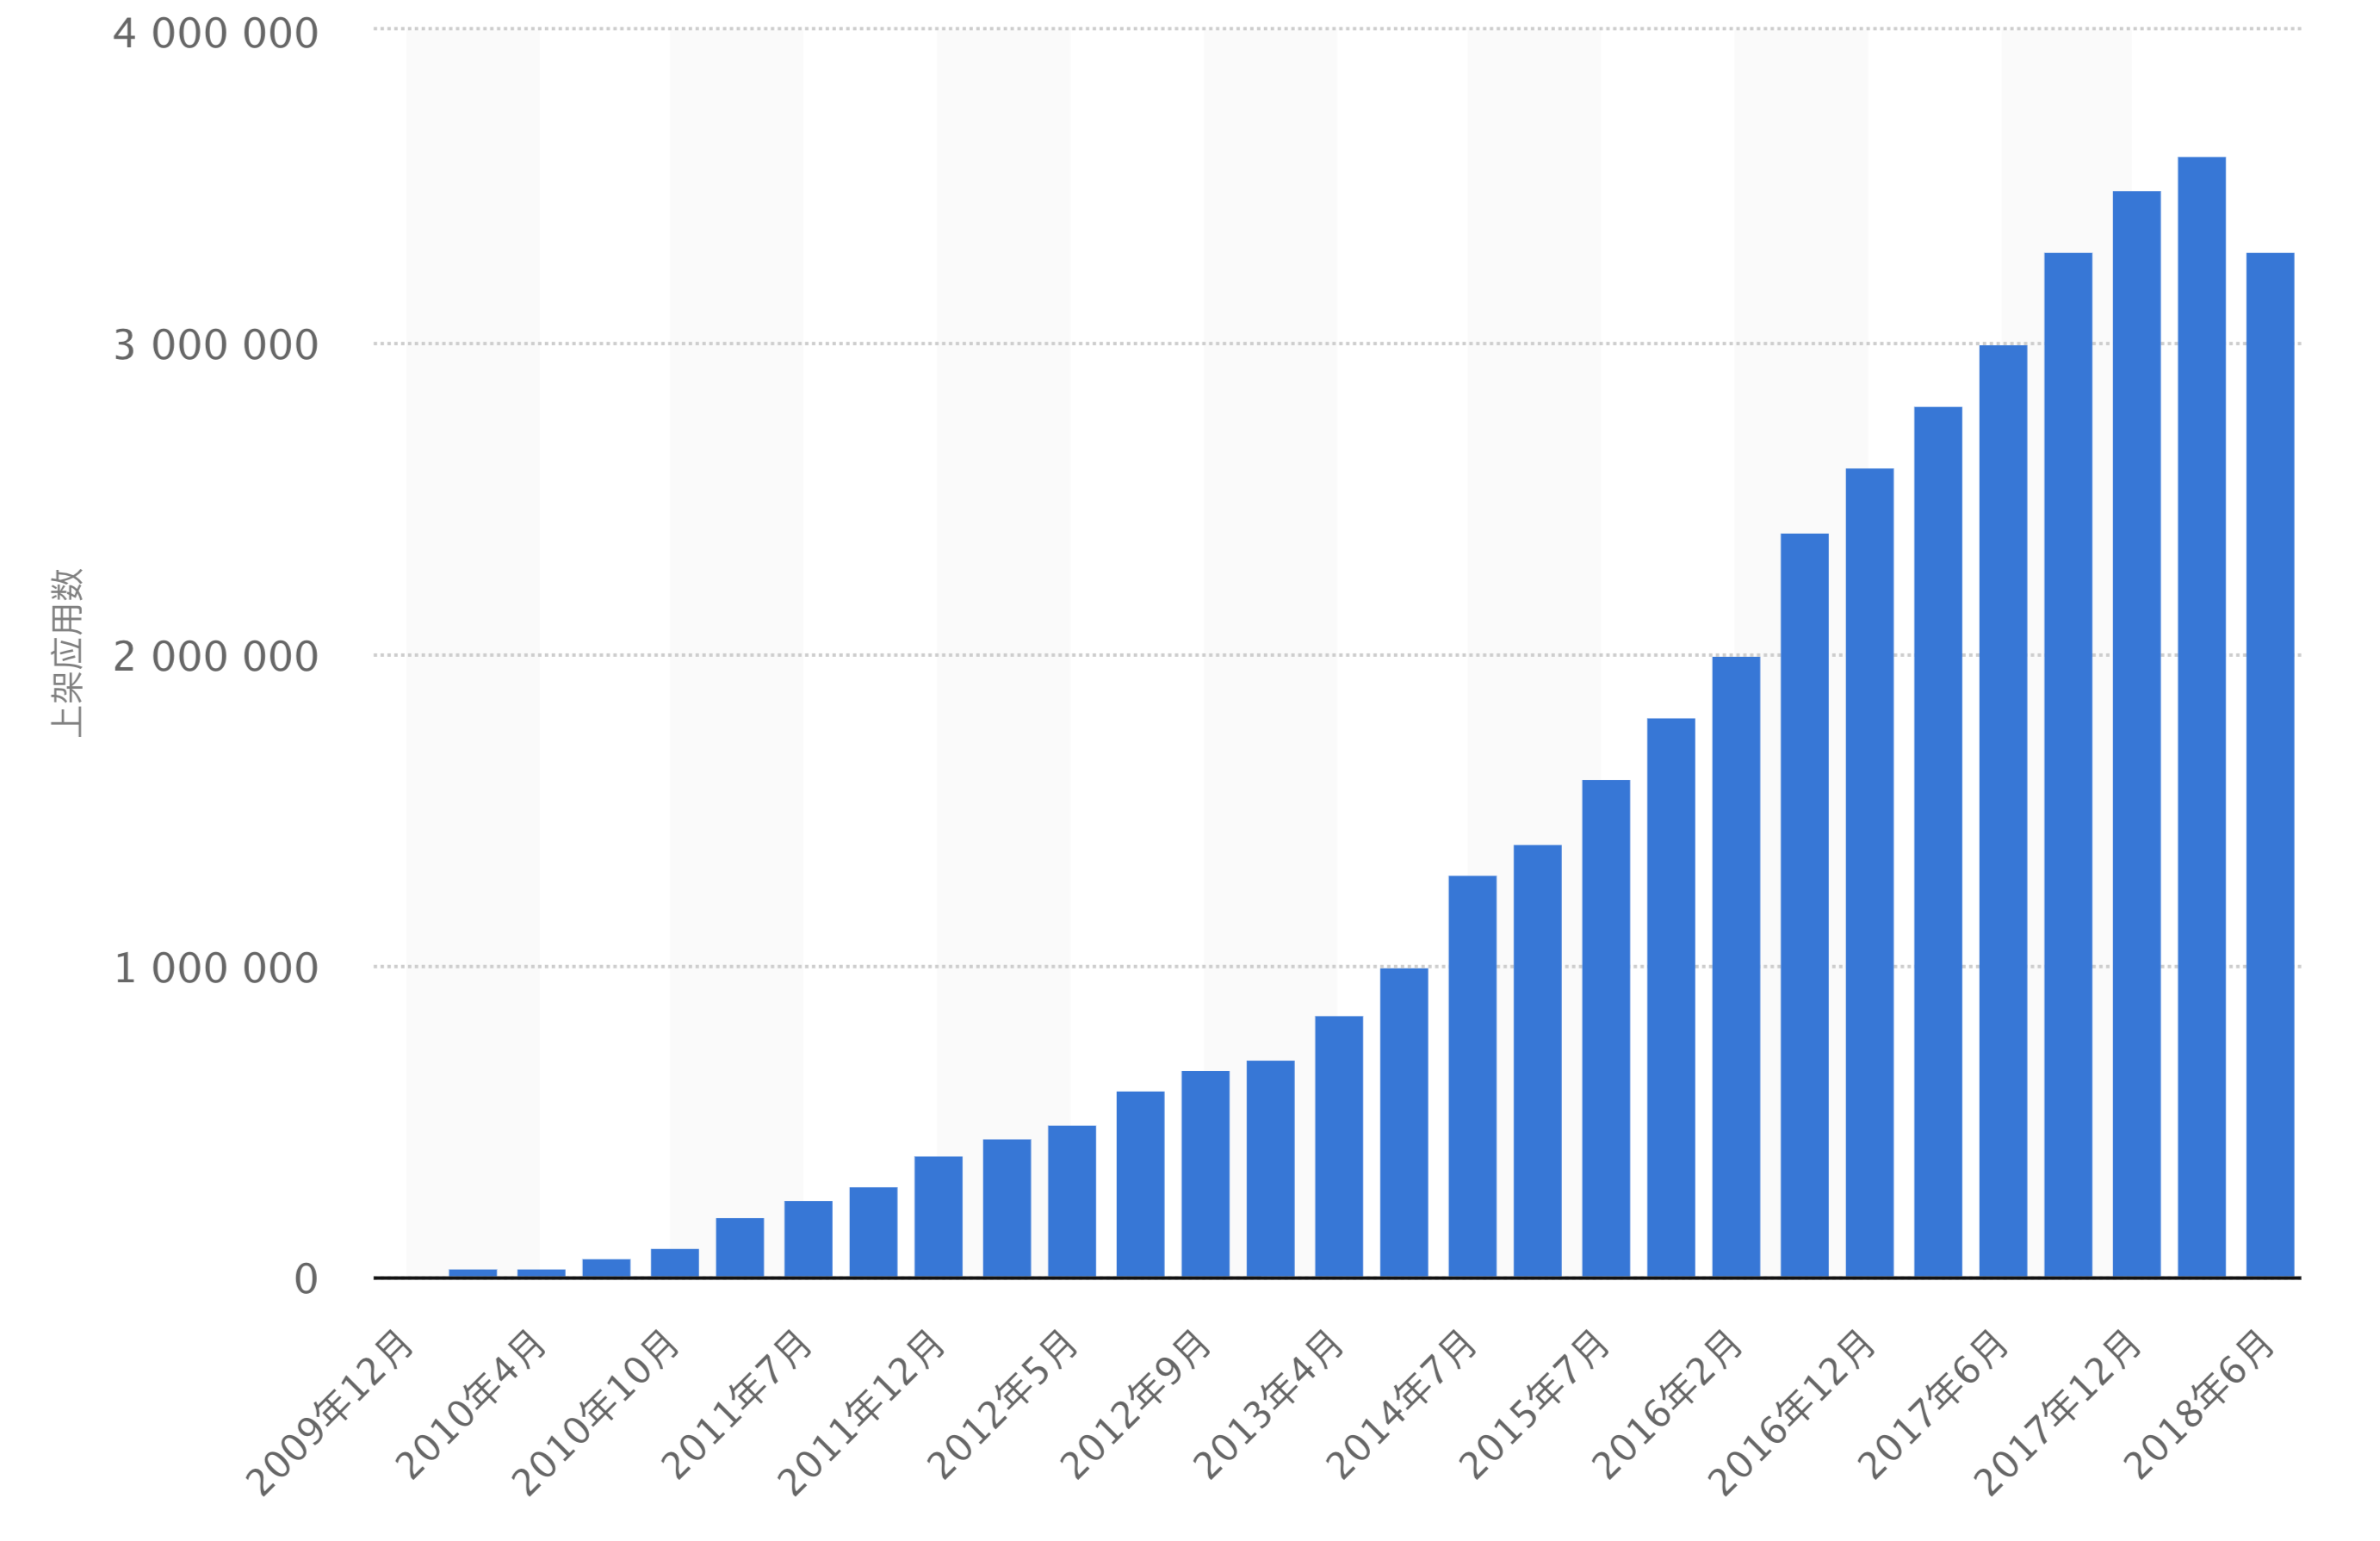
\includegraphics[width=\textwidth]{./Figures/app-numbers.png}
	\caption{Google Play Store上架的应用总数的变化趋势}
	\label{fig:app_number}
\end{figure*}


正因为移动应用迅猛的增长趋势,学术界和工业届的相关人员开始研究如何通过技术手段分析移动应用的代码内容,了解应用本身的运行时行为,进行相关学术研究和工业生产。
利用程序分析技术,研究人员对应用程序的项目相关源代码、配置文件或者二进制分发文件进行分析,监控程序的运行时行为,总结出应用程序相关特征。
结合具体应用场景,我们对这些特征进行归纳总结出相关规律,应用在应用分析、安全风险以及质量保障等领域,进一步提升应用程序的易用性、安全性和可靠性。

根据分析过程中是否需要运行目标程序,我们可以将这些技术手段分为静态分析技术和动态分析技术。
如果分析过程不依赖于目标程序的运行,这种分析技术称为静态分析技术,反之则为动态分析技术。
静态分析技术通常以二进制程序文件作为研究主体,结合相应的控制流分析、数据流分析技术、指针分析以及程序依赖分析,得出应用程序过程内的控制依赖和数据依赖(两者统称为程序依赖);
根据程序方法内相关函数/方法\footnote{在Java语言中,函数称为方法。在本文中,两者可以相互替换,不做区分。}调用,可以得到函数调用图、UML类图和序列图;
我们将程序依赖数据和函数调用图相结合,可以进一步得到过程间程序依赖~\cite{stafford2000formal},帮助研究人员了解程序整体层面的业务间的依赖关系,进行污点传播分析。
相反的,动态分析技术依赖目标程序的运行,通过修改目标程序的运行文件,搭建目标程序的运行环境,记录程序运行过程中相关操作信息,监控目标程序在运行过程中的状态变迁或指标变化,
进而得出程序在运行过程中的行为特定,帮助研究人员进行程序安全性分析,提升程序的质量可靠性。

但是,上述两种技术各有各的优劣。
静态分析技术有着较为扎实的理论基础,分析结果精确可靠,覆盖范围全面。
但是,静态分析技术在枚举所有情况时,往往会遇到状态爆炸的问题,具体实验效果受到实验运行环境的硬件条件和算法实现程度的限制。
而且,静态分析技术分析的问题依赖于外部环境(用户实时操作序列、手机所处环境因素,如温度等),分析得到的结果并不是非常准确。
动态分析技术却能解决这个问题,通过对程序运行状态的监控,研究人员可以了解程序的运行行为,掌握程序的安全性信息和可靠性信息。
但是,动态分析技术的缺点也非常明显:动态运行环境的搭建往往要设计到相关系统的源代码,构建系统的时间成本大,技术要求高。
另外,动态分析技术的分析结果往往只针对一次程序的运行过程,无法直接推广到其他运行情况。

Android应用程序的特性(例如,基于事件驱动的基础架构、面向组件的开发方式、高度依赖回调函数和多线程交互等)使得传统分析工具无法直接应用在Android程序上,对研究人员了解Android应用程序执行细节造成了一定的困扰。
为了解决这个问题,本文提出了一种静动态相结合的技术方案,通过程序源代码和运行环境进行预处理,获得程序的运行时信息,进而还原出Android应用程序的动态函数调用图。
在调用图中,除了方法调用关系,我们还提供了方法对象、方法间触发关系等信息,可以帮助研究人员补全函数关系,较为全面地了解应用程序运行时的状态变化。




\section{Android分析技术}

通常的,软件分析技术主要分为静态分析技术和动态分析技术两类。

\subsection{静态分析技术}

在不执行应用程序的情况下,静态分析技术通过对应用程序的源代码或者执行文件进行控制流分析和数据流分析,进而推断应用程序在运行过程中可能产生的行为。
这方面相关工具包括Soot~\cite{vallee1999soot}、FlowDroid~\cite{arzt2014flowdroid}、AmanDroid~\cite{AmanDroid}、IccTa~\cite{iccta}、androguard~\cite{androguard:online}等。
Soot是传统的静态分析工具,其思路是将所有的Java字节码文件转化成一种中间语言Jimple,并在Jimple的基础上进行常规的控制流分析、数据流分析,理论上适用于所有可以在Java虚拟机上运行的语言(例如Scala、Groovy等等)的分析。
由于Android程序本身的字节码Davlik和Java字节码在格式上保持一致,因此,Soot也支持Android应用程序的静态分析。
但是,Soot在分析过程中没有考虑一些Android的特性难免会出现一些问题。
为此,德国达姆施塔特工业大学的Steven Arzt等人在Soot的基础上考虑Android程序中Activity的生命周期特性,推出了一个针对Android的静态分析工具FlowDroid,可以做到上下文、路径、对象、字段等层面上的敏感。
FlowDroid通过定义数据源点和数据泄漏点,在Android应用生命周期的基础上,可以实现数据流敏感的污点分析。
但其不足之处在于缺少跨组件通信的分析不考虑多线程调用问题。
在FlowDroid基础上,卢森堡大学的Li Li等人推出了IccTA,利用跨组件通信分析工具IC3提取跨组件通信(Inter-Component Communication, ICC)的方法调用,并结合AndroidManifest.xml文件定义的Intent Filter信息,连接ICC两端的组件,克服了FlowDroid因缺少跨组件通信而导致的数据流上的缺失。
因为它是构建在FlowDroid之上的一个探测敏感信息泄露的,所以受限于FlowDroid的局限性。

Yang等人~\cite{yang2015static},利用静态分析技术,并将回调函数添加到控制流图(调用图)中,形成了回调控制流图(Callback control-flow gragh)。
实验结果显示,Yang的工作比Gator~\cite{rountev2014static}在控件监听器绑定上得到了更为准确结果。
法国和意大利的学者~\cite{payet2012static}通过对Java字节码静态分析器Julia进行扩展,使得其支持对 Android 应用程序的静态分析;
他们通过改写 Android 库中 Activity、LayoutInflater 等类的代码逻辑,规避了Android系统分析常见难点(如程序的事件机制,基于反射的视图加载等),
实现了包括死代码检查、空指针检查在内的7种静态分析技术。



%由此可见,静态分析工具在分析过程中虽然可以对应用程序进行较为全面的分析,覆盖应用程序的所有代码,但由于缺少和程序执行过程相关的部分必要信息(应用程序的执行序列、和设备所处环境相关的传感器(如GPS、温度等)信息等),可能导致部分情况下分析结果的不精确。为了解决这一问题,研究人员提出了动态分析技术。


\subsection{动态分析技术}

% 为了解决这一问题,研究人员提出了动态分析技术。
和静态分析技术相对应,动态分析技术通过执行应用程序,获取程序运行过程的相关信息,从而实现对应的研究目的。
动态分析技术往往需要对运行环境做适当的修改或者调用特殊的系统接口,记录应用程序运行过程的关键信息,结合数据流追踪等技术,已记录应用程序的运行时行为。
这方面的工作代表包括TaintDroid ~\cite{chun2014taintdroid}、DroidBox~\cite{droidbox:online}、TraceDroid~\cite{van2013dynamic}、DroidScope~\cite{droidscope}等。
Enck等人提出的TaintDroid,是一个高效的系统级的动态污点跟踪和分析系统。它通过修改Dalvik虚拟机,利用动态污点分析技术实时监控敏感数据的生成、传播和泄露,实现了变量层面、方法层面、文件层面的数据追踪。
此外,TaintDroid还支持跨进程通信(IPC)层面上的污点分析,因此可以精确分析出应用程序从消费者手机上获取和发布隐私信息的完整传播过程。
TaintDroid提供了较为完备的数据流分析技术,但是不支持控制流追踪,无法给出相关语句的执行路径。
DroidBox在TaintDroid基础上,对Android Framework的部分API做了修改,可以记录一些开发人员感兴趣的API(例如文件读写、网络请求、SMS服务等)的调用,并提供分析结果的可视化。
同时,DroidBox还实现了应用程序的自动安装和执行,弥补了TaintDroid在软件测试自动化方面的不足。
和TaintDroid不同,TraceDroid采用的是另一种思路,利用字节码插装技术AspectJ,使得方法在执行时输出相应的日志信息。根据这些信息TraceDroid可以还原函数调用图,得到分析结果。
由于Aspect在进行字节码编织时引入的新的方法会导致生成源APK文件中的方法总数超过65536~\cite{Configur27},进而使得APK文件无法成功构建,因此该方案存在不稳定的情况。

另外,研究人员还用动态分析技术查找Android应用程序在运行时性能瓶颈。Android官方性能检测工具SimplePref~\cite{simpleperf:online}就是其中的一个代表。
SimplePref利用了Linux提供的系统接口pref\_event\_open,定时获取到性能监视单元的相关信息(例如cpu周期数、执行的指令数、缓存失效次数等)。
利用这些信息,SimplePref可以得到对应时刻的CPU状态,还原出各个方法的执行时间和对应的执行路径。
根据方法执行时间的长短和对应的执行路径,开发人员可以发现程序的性能瓶颈,进而通过对程序代码做出调整,提升程序的运行性能。
但是,该方法受到系统接口回调周期的影响,过于频繁的调度周期会使系统产生过大的开销,影响原有程序的执行;反之,则会丢失部分方法的执行信息。
而且,Android程序关心的性能瓶颈一般都位于主线程,而SimplePref会输出所有线程的执行信息,实际开销较大。
为此,Uber的Nanoscope~\cite{ubernanoscope:online}采用追踪(Trace)技术在定制化的系统Nanoscope OS中运行,在虚拟机解释执行目标方法前后输出相关Trace日志,进而得到性能报告。
相比SimplePref,Nanoscope只输出主线程相关的方法数据信息,大大减低了性能上的开销。
但是,nanoscope的局限性在于构建成本较高,需要配合特定的系统使用。




\subsection{分析技术的应用}
\textbf{应用分类:}

Simapp~\cite{chen2015simapp}

mobile app tagging ~\cite{chen2016mobile}

WhyPer~\cite{pandita2013whyper}


\textbf{安全性分析:}


AppContext~\cite{yang2015appcontext}

AppIntent~\cite{yang2013appintent}

Socket~\cite{bu2017program}


\textbf{质量保障:}


Exception fault localization in Android applications~\cite{mirzaei2015exception}

machado2013mzoltar~\cite{machado2013mzoltar}


Fan~\cite{fan2018efficiently,fan2018large}

% 例如错误定位、自动化分析、profiling等

\section{本文的主要工作}

本文的主要研究工作包括以下:

1)	调研最近几年Android应用分析领域的静动态分析工具,了解各项工具的优劣以及相关的应用案例。

2)	提出并实现Android动态函数调用图构建系统,包含传统函数调用图的构建以及在此基础之上的多线程函数调用关系的构建。

3)	对上述系统设计对应的实验方案,评估对应的实验效果。

\section{本文的组织结构}

本文共分为六章,环绕着Android动态函数调用图构建系统的设计与实现展开,各章节内容如下:

第一章:主要介绍了本文的主要研究背景、主要工作内容以及研究意义,最后对本文的各章的内容做了阐述。

第二章:从Android的体系结构出发,并由此展开介绍了最近几年Android领域相关的静态分析技术和动态分析技术,以及这些技术在各自领域的运用,简单描述本文可能遇到的困难。

第三章:从系统功能、技术路线、技术选型、模块实现等若干方面介绍RunDroid的设计与实现。

第四章:从应用程序的构建效率、日志本身记录效率以及系统对程序运行的影响等三个方面设计并开展相关的测试实验。

第五章:将展示RunDroid系统生成的函数调用图的运行结果,并对函数调用图进行详细的阐述。

第六章:对本文工作进行总结,并对下一步工作进行展望。


\chapter{Android系统相关背景介绍 }  
\label{ch2}


本章首先会简要介绍Android系统架构,其次会对Android中的Activity组件做基本介绍,接着会着重介绍Android中常见的两种多线程交互方式,最后将指出本文系统在实现上的难点。

\section{Android系统结构介绍}

Android是基于Linux内核开发的的开源操作系统,隶属于Google公司,主要用于触屏移动设备如智能手机、平板电脑与其他便携式设备,是目前世界上最流行的移动终端操作系统之一。

在系统架构上,Android自下到上,可以分为四层:Kernel层、Library和Android Runtime(Dalvik/ART)、Framework、Application等,如~\autoref{fig:Android-Framework}所示。
Kernel层是硬件和软件层之间的抽象层,主要是设备的驱动程序,例如:显示驱动、音频驱动、蓝牙驱动、Binder IPC驱动等。
Library和Android Runtime(Dalvik/ART): Library,顾名思义就是向上层提供各种这样的基础功能,例如SQLite数据库引擎,Surface Manager显示系统管理库。
Android Runtime主要是运行Android程序的虚拟机,在不同版本的系统上对应着不同的虚拟机,例如在Android 5.0及以上是ART,而在Android 4.3及以下是Dalvik,而Android 4.4两者都有。
Framework层主要是系统管理类库,包括Activity的管理,消息通知的管理;同时,它是Application的基础架构,为应用程序层的开发者提供了API,其存在简化了程序的开发。
而Application就是我们平时接触的应用,开发人员公国调用底层Framework提供的API实现相应的接口。

虽然Android应用程序是使用Java语言开发的,但是它和传统的Java程序有着很大的不同,具体有如下几点:

\begin{figure*}
	\centering
	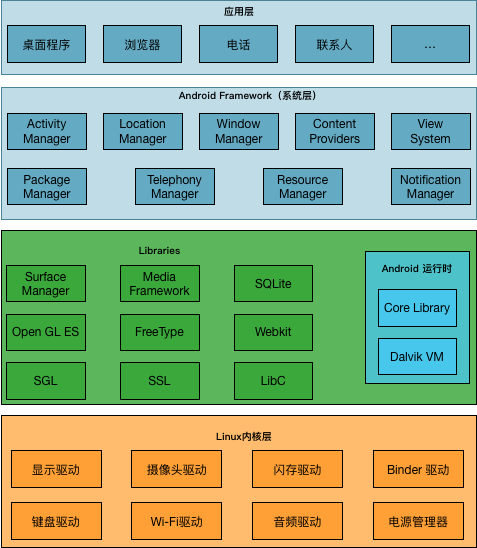
\includegraphics[width=\textwidth]{./Figures/Android-Framework.png}
	\caption{Android系统框架图}
	\label{fig:Android-Framework}
\end{figure*}


\textbf{基于事件驱动的编程模型:}
在设计上,Android应用程序的开发架构采用的是事件驱动架构。在开发过程中,没有传统程序中入口函数Entry Point的概念。应用程序中通用的业务逻辑(例如应用程序如何启动退出、应用的窗口如何创建销毁等)存在于Android Framework中。这也使得Android应用程序的分发文件(即APK文件)相对较小。

\textbf{面向组件的开发方式:}
Android程序中较为常见的是组件(Component,例如Activity、Service、Content Provider、Broadcast Receiver),它是应用程序运行的最小单元,受到Android Framework的直接调度。开发人员通过继承这些组件,重写对应的生命周期函数,已实现对应的业务需求(界面的布局、页面状态的保存等),而这些组件的生命周期由Framework调度完成。

\textbf{大量逻辑实现依赖于回调函数和多线程通信:}
由于Android应用程序采用的是基于单线程消息队列的事件驱动架构,因此,界面相关的操作只允许出现在主线程(UI Thread)中,耗时操作只能在工作线程(Worker Thread)中进行。通常的,开发人员往往会借助回调函数处理控件的响应事件,利用多线程交互串联界面相关操作和耗时操作,完成对应的业务。


\section{Android中的Activity}

在Android应用程序运行过程中,Activity向用户展示图形界面,响应用户的反馈,和其他组件一同完成相关业务,扮演着最为重要的作用。由于Android应用程序在架构选型上采用了事件驱动模型,为了便于协调应用内部状态的管理,Android组件通常有生命周期的概念,Activity也不例外。

Android系统根据Activity 在运行时和用户的反馈将其状态分为以下四种:
\begin{enumerate}
	
	\item 运行态:在该状态下, Activity处于页面最前端时,用户可以与Activity进行交互。一般的,我们看到Activity均处于这个状态。
	
	\item 暂停态:在该状态,Activity仍然可见,但是失去了窗口的焦点。当一个Activity之上出现一个透明的Activity、Toast或者对话框时,Activity就处于这个状态。处于暂停状态的Activity仍处于存活状态,保存着所有的内存数据,只有当系统内存极度紧张时,才有可能被系统杀死回收。
	
	\item 停止态:当一个Activity被其他的Activity遮挡时,处于这个状态。处于该状态的Activity仍然可以保留所有的状态,只是对用户不可见。系统在需要内存的情况下,可以采用相应的策略对Activity进行杀死回收操作。
	
	\item 终止态:当Activity处于暂停态或者停止态时,系统由于内存原因可能会将上述两种Activity杀死回收。处于该状态下的Activity将不能直接恢复。
\end{enumerate}

Activity的生命周期就是以上状态之间的跳转,受到Activity在运行时的内存分布、环境状态以及业务逻辑的影响,由Android系统直接负责调度。
Android系统为Activity提供了onCreate(), onStart(), onResume(), onPaused(), onRestart(),  onStoped()和onDestroy()等方法,方便开发人员在Activity的状态发生变化时对程序的运行时数据和应用状态做适当的处理操作。对应的Activity的生命周期具体如~\autoref{fig:Activity-lifecycle}所示:


\begin{figure*}
	\centering
	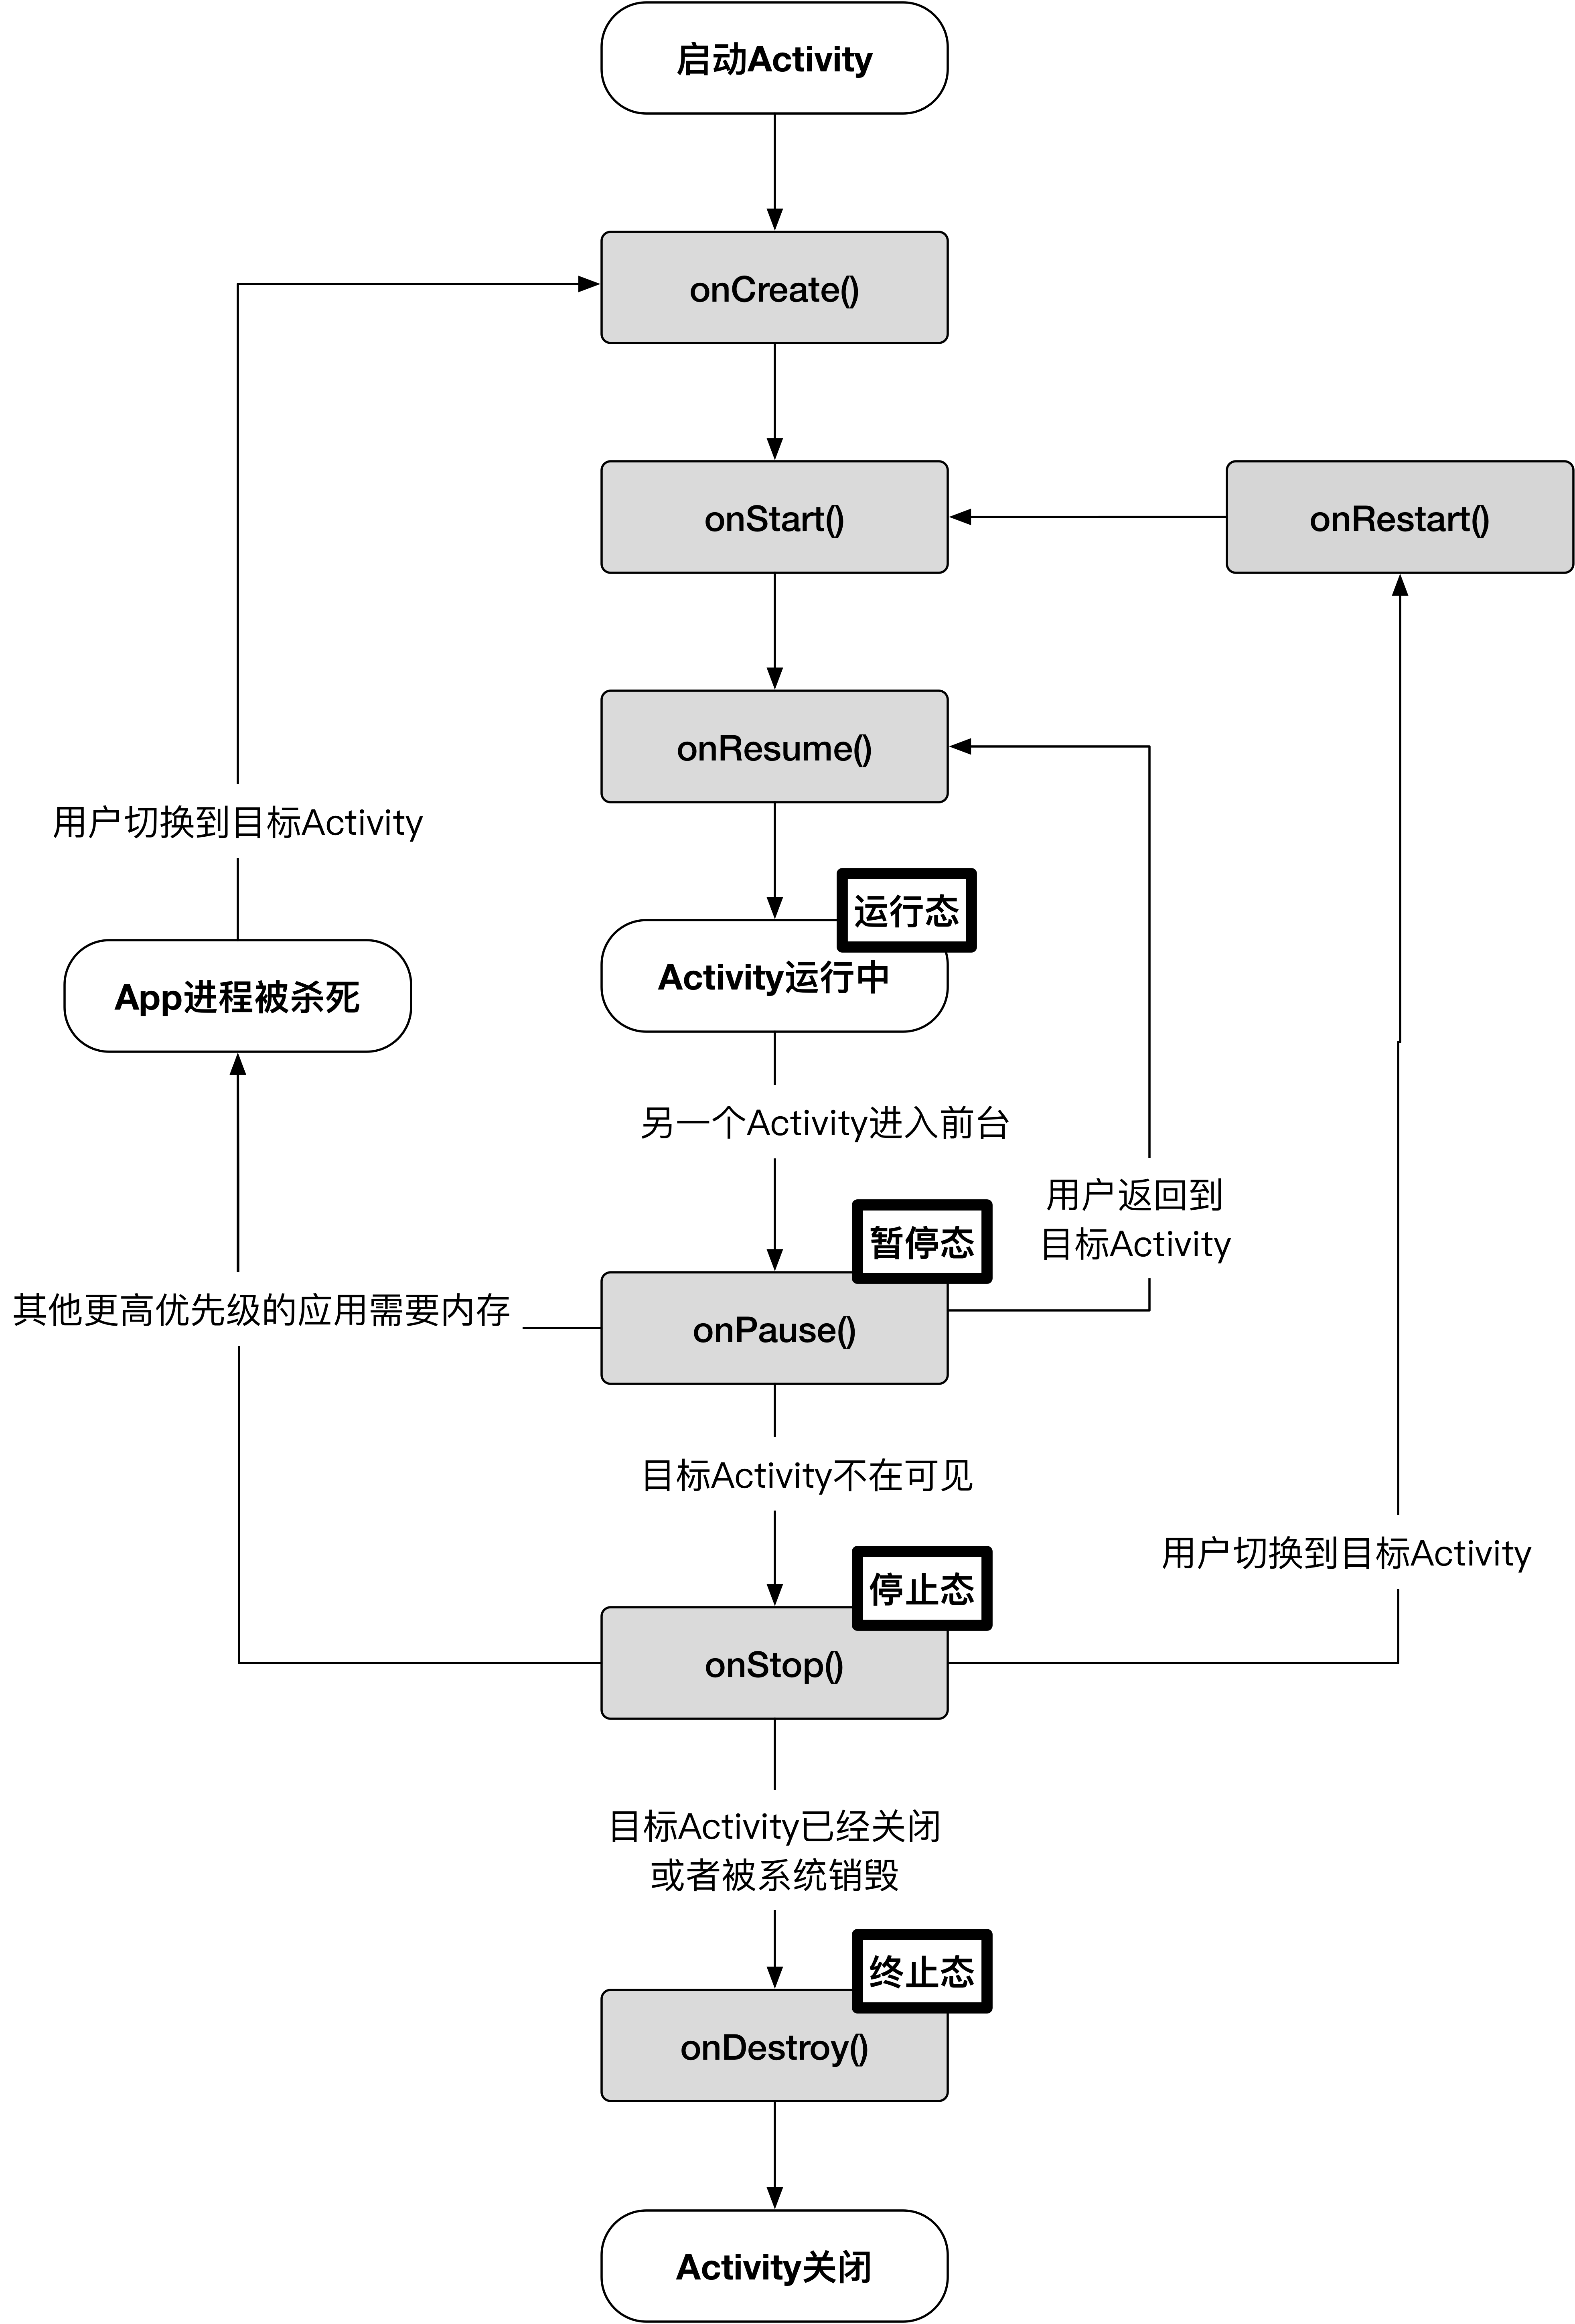
\includegraphics[width=\textwidth]{./Figures/Activity-lifecycle.png}
	\caption{Activity的生命周期}
	\label{fig:Activity-lifecycle}
\end{figure*}


当用户点击应用图标,系统启动应用程序后,系统会创建Activity、启动Activity并使之可以和用户进行交互,在这个过程中,onCreate()、onStart()、onResume()等方法被回调,Activity最终处于运行态;

当用户点击“返回键”返回到桌面时,Activity会失去焦点,在用户的视野中消失,直至被系统回收,对应的状态也从运行态经暂停态、停止态,变为终止态变,期间onPause()、onStop()、onDestroy等方法被回调;

当用户从一个界面回到原来的界面时,原有的Activity从停止态重启,先后出现在设备界面上,获得和用户交互的焦点,期间onRestart()、onStart()、onResume()等方法被回调;

当一个Activity长期处于停止态,但由于内存原因被系统回收时,用户尝试启动它时,系统会像启动一个新的Activity一样启动它。

\section{Android中的多线程交互}
Android系统在架构设计上采用了事件驱动架构。在多线程并发访问时,若UI控件对于各线程均是可见的,并发对控件做读写操作会使控件处于不可预期的状态;若贸然对控件使用锁机制,这将会使阻塞部分线程业务逻辑的执行,使得应用变得复杂低效。上述情况对于应用程序都是不可接受的。为了避免多线程操作之间的竞争关系带来的低效率问题,Android系统在设计事件驱动架构时,采用了单线程的消息队列,即只允许在主线程(也称为主线程,Main Thread)进行界面更新操作,不允许在其他线程(也称为工作线程,Worker Thread)进行界面更新操作。

当应用程序出现耗时操作(例如加载磁盘上的图片、网络请求等)时,应用程序往往需要在一个新的线程中执行上述逻辑。当应用程序界面中的某些控件需要根据耗时操作的结果(例如渲染得到的图片对象、网络请求得到的JSON字段)更新界面状态时,开发人员需要切换到主线程进行界面的更新。

从整体上,开发者可以需要的交互方式分为基于Java的多线程交互和基于Handler的交互方式。

\subsection{基于Java的多线程交互}

由于Android系统提供的API接口兼容Java多线程相关的部分API,因此,在Android系统中,开发人员可以采用和Java应用相同的调用方式启动工作线程,并在对应的线程上完成业务逻辑。但是,Java API只能实现业务逻辑从原有线程转移到新的工作线程上,不能重新返回到主线程上。为此,Android系统在Java API的基础上还提供了void runOnUiThread (Runnable action) API。runOnUiThread API可以帮助开发人员将业务逻辑的执行从工作线程转移到主线程上,该API也符合Android只允许在主线程上更新界面这一基本设计原则。但是,该API也存在着一些弊端,例如runOnUiThread API的定义位于类android.app.Activity,这也就意味着在Android组件Service中进行耗时操作时,无法通过该API返回到主线程;同时基于接口的函数参数定义方式对于跨线程的参数传递也不是十分友好。为此,Android提供了基于Handler的多线程交互方式。

\subsection{基于Handler的多线程消息调度}

为了满足开发人员多样化的业务在多线程间的切换,Android提供了基于Handler消息调度的多线程交互方式。当开发人员需要当前业务逻辑转移到其他线程时,通过方法Message.obtain()获取一个Message,将对应的业务逻辑封装成Runnable对象传递给Message中对应的字段,或者将对应的参数传递给Message中的参数字段,最后通过Handler对象发送给指定的消息队列。当目标线程的消息队列读取到这条消息时,便会在该线程中执行预定的业务逻辑。

~\autoref{fig:handler-code}为Handler的简单示例:用户在工作线程执行一项耗时任务(生成一个字符串),将生成的字符串传递给Message对象,并通过Handler对象通知主线程进行界面更新。


\begin{figure*}[h]
	\centering
	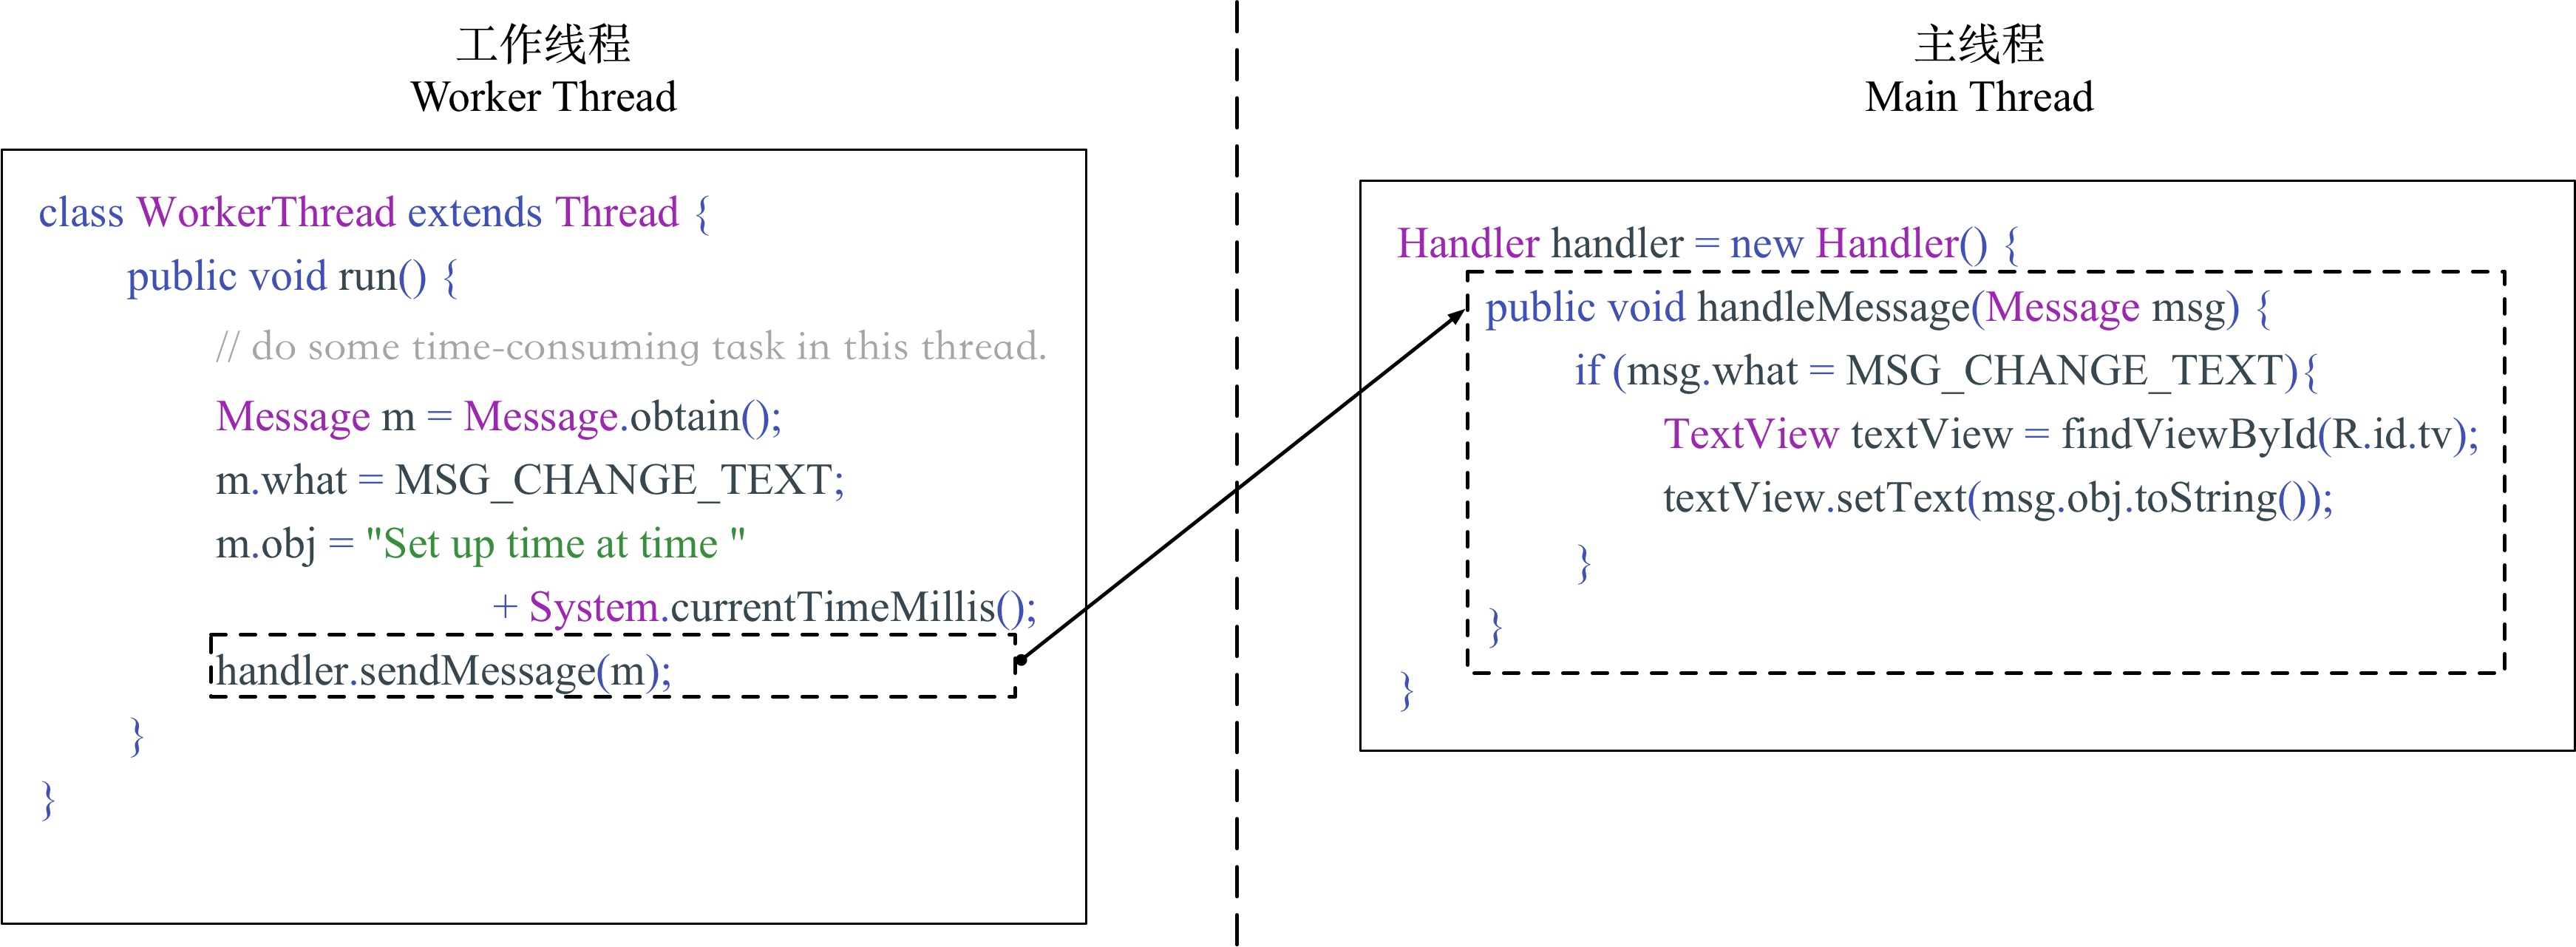
\includegraphics[width=\textwidth]{./Figures/handler-code.png}
	\caption{Handler的使用实例}
	\label{fig:handler-code}
\end{figure*}


从Android SDK提供的API来看,开发人员可以通过post(Runnable),postAtTime(Runnable,long),sendMessage(Message),postDelayed(Runnable, Object, long), sendMessageDelayed(Message,long),sendMessageAtTime(Message,long)和sendEmptyMessage(int)等多种API形式实现消息调度。通过查阅和分析Android系统相关源代码,我们发现上述Handler相关的API关系如~\autoref{fig:handler-apis}所示。


\begin{figure*}[h]
	\centering
	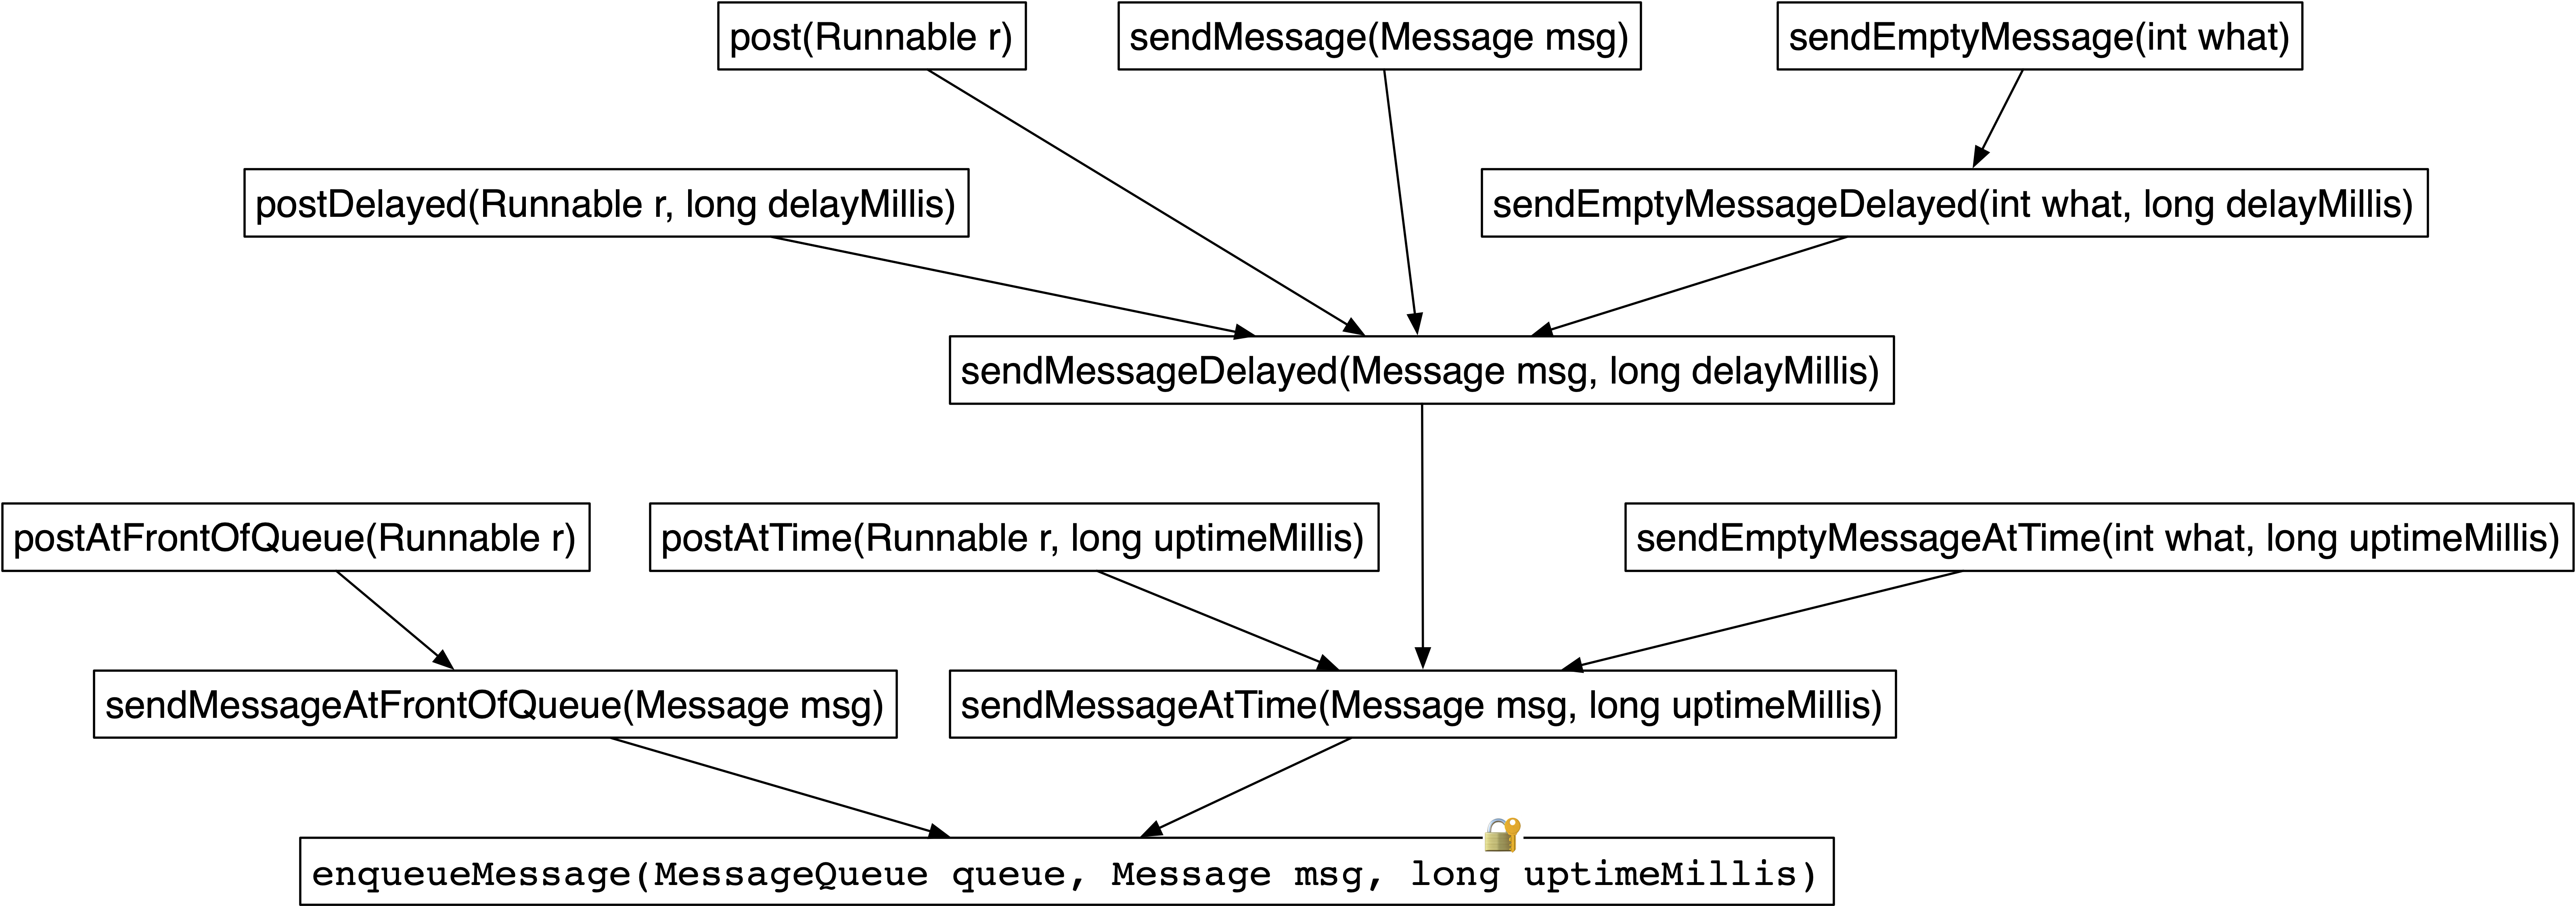
\includegraphics[width=\textwidth]{./Figures/Handler-apis.png}
	\caption{ Handler 各API之间的调用关系}
	\label{fig:handler-apis}
\end{figure*}


从~\autoref{fig:handler-apis}中,我们可以发现所有的API最后就会调用到android.os.Handler enqueueMessage(MessageQueue, Message, long)方法。

从底层实现上看,Handler机制主要由Handler、Looper、MessageQueue、Message等若干部分组成。Message是跨线程交互的主要载体,Android系统采用对象池的设计模式来管理Message对象;无论开发人员以何种形式调用了Handler发送消息,传递的参数最后均会封装到Message对象中。MessageQueue则存放着所有待处理的Message对象,它是一个双端队列,开发人员可以根据具体业务场景在消息队列的头部、尾部或者适当位置插入消息队列。Looper则负责以epoll的方式从MessageQueue中循环读取Message对象,分发给对应的Handler对象使得业务可以在对应恰当的线程上被处理;一个线程最多只允许只有一个Looper对象,他只能绑定一个与之对应的MessageQueue;其中最为常见的就是位于主线程的MainLooper,它主要负责Android系统的日常调度(例如Activity的生命周期、控件的点击事件响应等)。Handler对象则负责将消息发送到对应的MessageQueue中(扮演着消息的生产者角色)以及消费来自Looper分发下来的Message(扮演着消息的消费者角色);在一个应用中,Handler可以存在多个对象,一个Handler对象也可以同时扮演生产者和消费者两个角色。

从原理上看,基于Handler的多线程消息调度,充分利用了Android的事件驱动架构,将业务逻辑抽象出Message对象。该消息对象通过Handler的对应接口发送至在目标线程所对应的消息队列MessageQueue中,再由Looper对象在目标线程运行时从消息队列中取出,分发给对应的Handler执行,达到了Android跨线程交互的目的。具体地,Handler的工作原理如~\autoref{fig:handler-framework}所示:


\begin{figure*}[h]
	\centering
	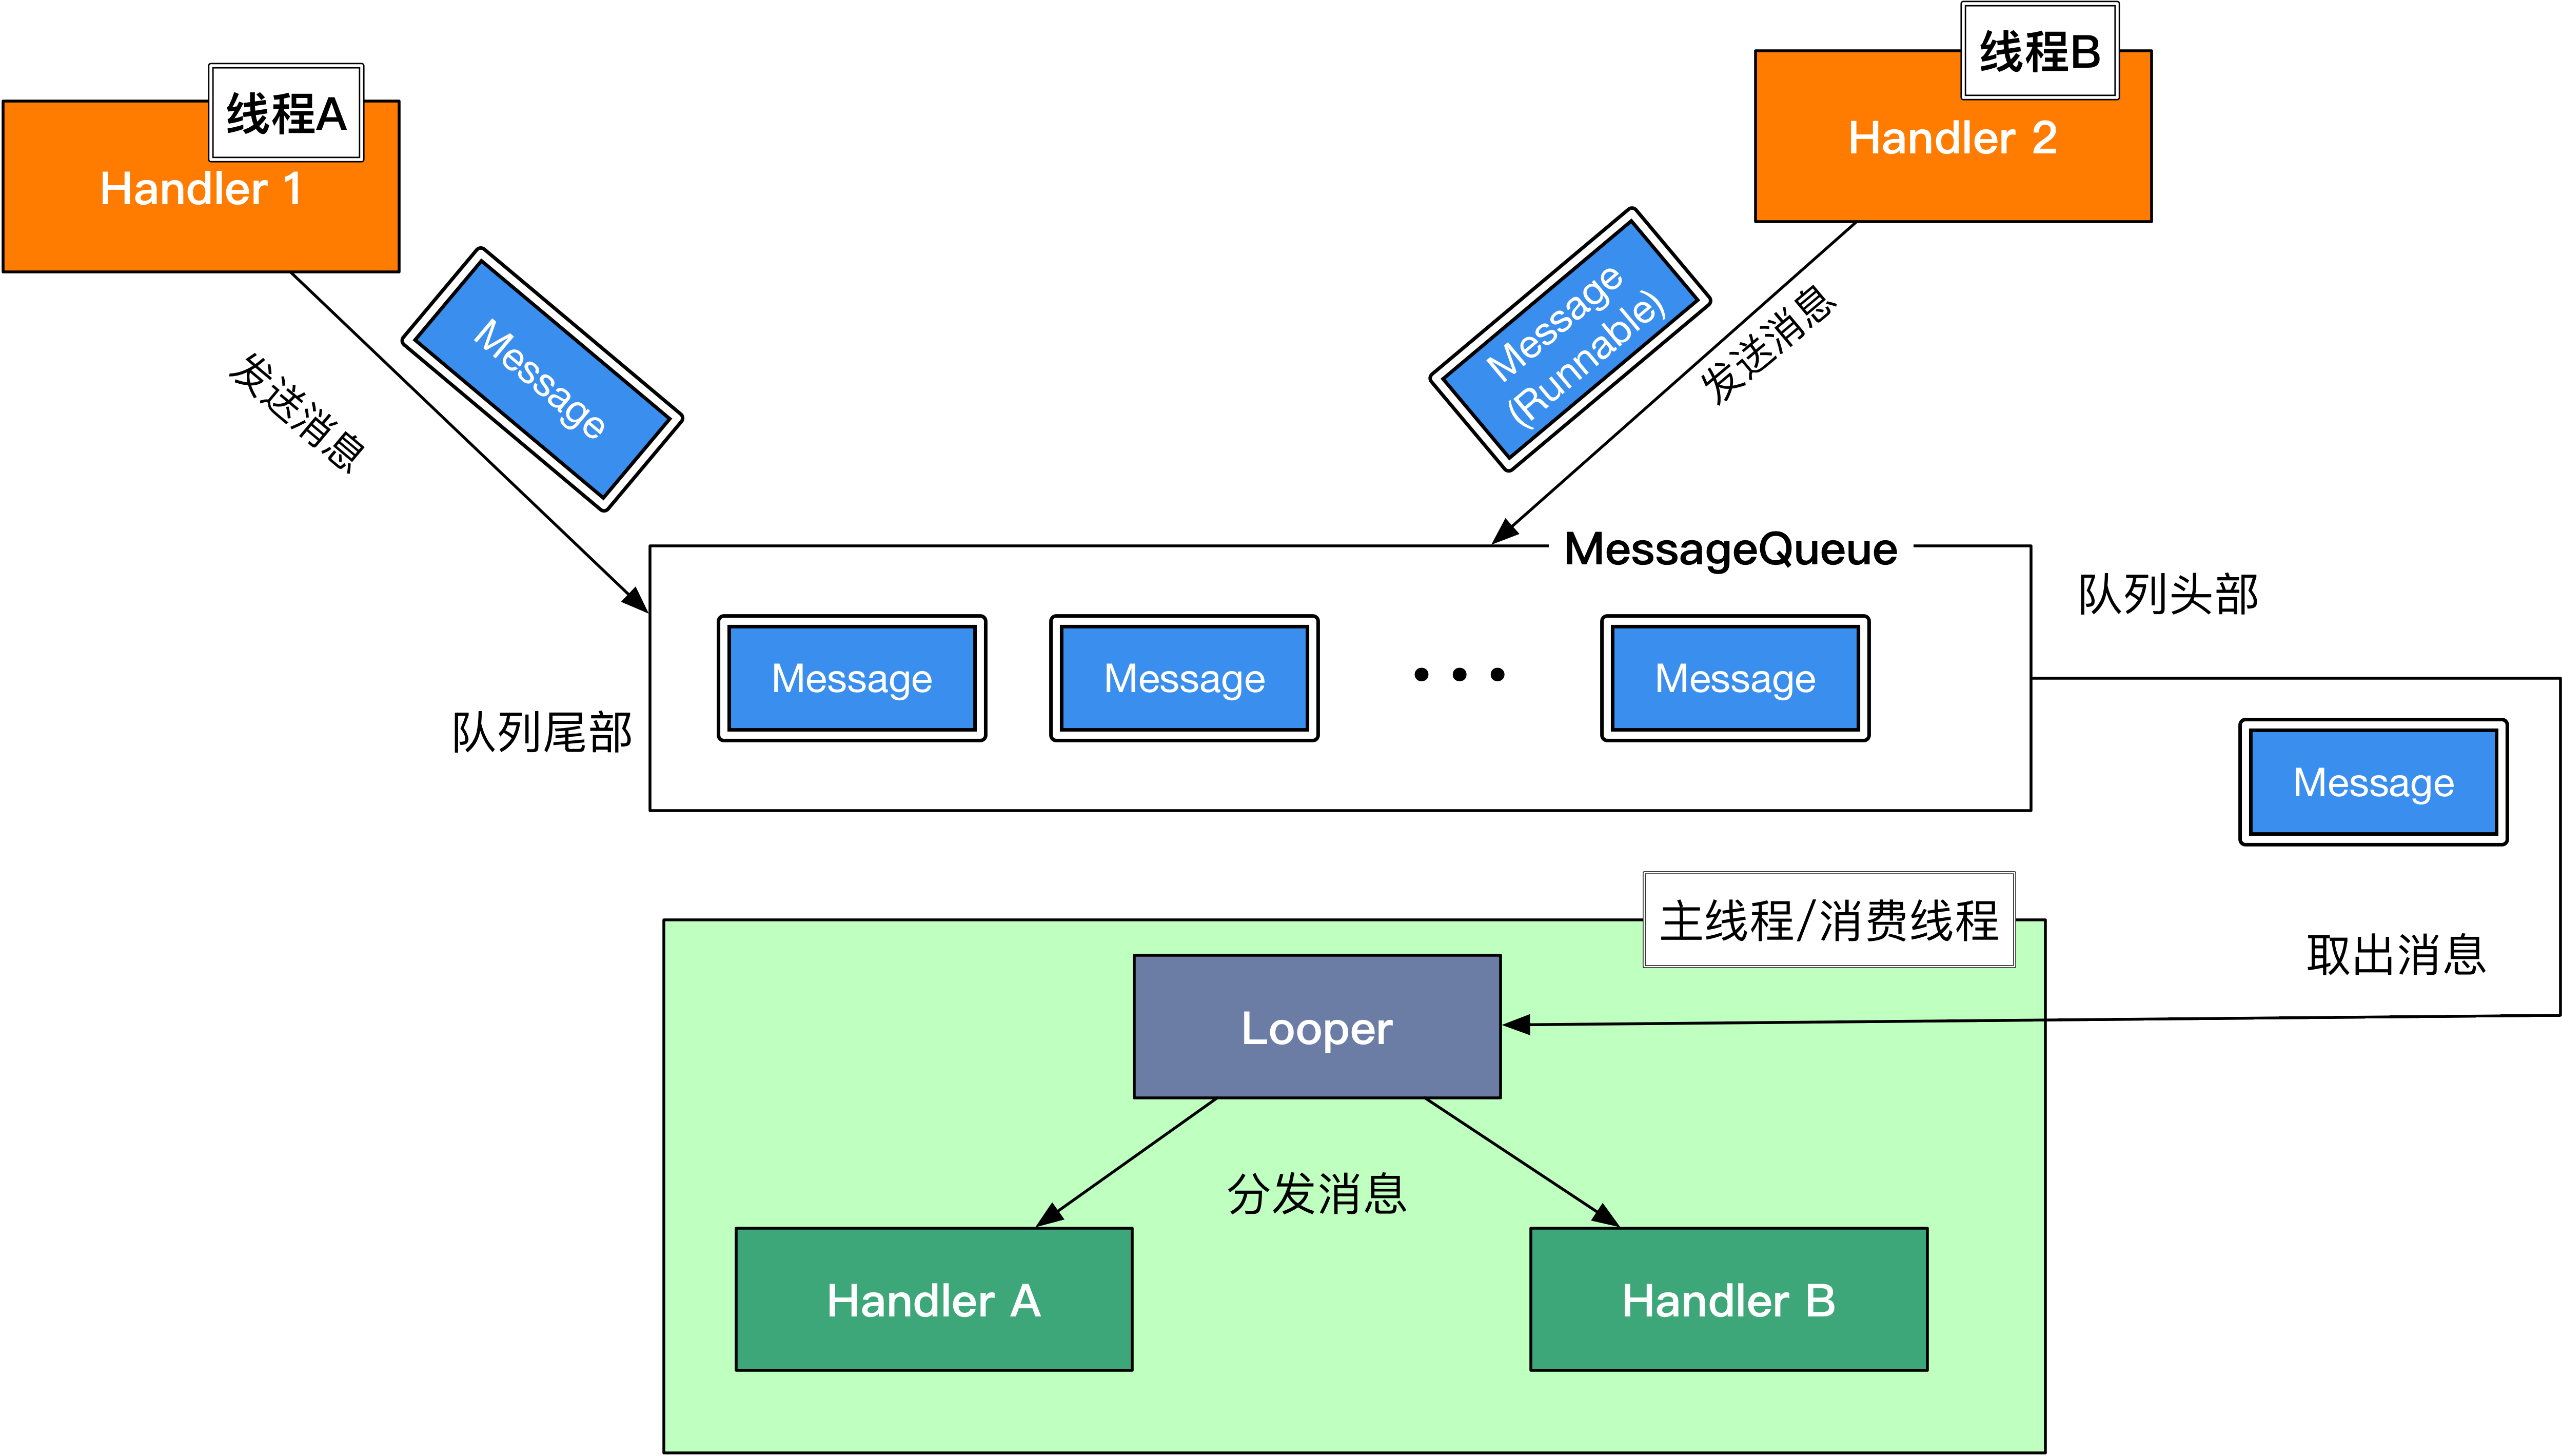
\includegraphics[width=\textwidth]{./Figures/Handler-framework.png}
	\caption{ Handler的工作原理}
	\label{fig:handler-framework}
\end{figure*}


综上所述,基于Handler消息调度的多线程交互方式,不仅可以帮助开发人员实现业务逻辑在主线程和工作线程间的自由转移,而且其灵活的API设计还帮助开发人员降低应用的设计复杂程度,提升了系统架构的可拓展性。因此,在Android开发过程中,基于Handler消息调度的多线程交互十分常见。
\section{本文遇到的困难与挑战}


本文解决的关键问题有如下几点:

1)	如何获取应用程序中各个函数的执行信息?

获取应用程序在执行过程中各函数执行信息是本文的基础。从函数分类上,用户定义的方法和系统预定义的方法。对于前者,我们可以通过修改程序源代码实现;但对于后者,由于我们无法直接修改系统程序的源代码或者构建一个符合本文业务需求的系统的成本较高,为此,我们需要寻找对应的解决方案以帮助我们获取系统方法的执行信息。

2)	如何根据程序中各函数的的执行信息,还原应用程序的函数调用图?

基于第一点,我们可以获取程序在运行过程中的执行信息。但仅仅依靠这些执行信息是不够的,我们还需要将这些执行信息组织起来,挖掘执行信息之间的关联关系,从而才能还原成应用程序的函数调用图。这将是本文研究的重点之一。

3)	如何在生成的函数调用图中体现Android特性?

正如上文所提的,Android系统中有很多常规应用中不具备的特性,例如Activity的生命周期、基于多线程调用的触发关系。若要在生成的函数调用图上体现上述特性,需要对Android系统源代码有一定的了解熟悉,并基于图中的相关信息创建与特性相对应的关系,这既是本文研究的重点,也是本文的创新点。

\section{本章小结}

本章主要介绍了Android系统的相关背景知识,较为详细的阐述了Android的系统结构,详细介绍了Android四大组件之一的Activity机器生命周期。同时,本章还介绍了基于Runnable/Thread、Handler消息调度两种不同的多线程交互方式,较为详细地分析了Handler的运行机制,为下文基于函数调用图的多线程触发关系生成做了铺垫。最后,本章还介绍了系统在实现上可能遇到的困难。


\chapter{面向CPES的MARTE扩展}
\label{ch3}
	对于智能建筑这类CPES,能量是关注的重要元素。只要系统在运作,就会造成能耗(Energy Consumption)。不同情境下,能耗的速率可能不同,如汽车的加速行驶比匀速行驶在单位时间内更加耗能。除此之外,系统也可能会产生能量(Energy Harvesting),能量的来源多种多样,包括热能、声能、动能、生化能\citep{DBLP:conf/iimss/SaidaKBA16}等。
	
	与一般系统相比,除了密切关注能量,CPES还具有以下两个典型特征:
	\begin{itemize}
	\item 混成是CPES的一个重要特性,由于CPES处于物理环境中,系统必然是连续行为和离散行为、连续变量和离散变量共存的。
	\item 开放的物理环境中存在各种随机行为,如天气的变化、用户行为等都是典型的随机事件。
	\end{itemize}

	因此,为了完整建模CPES,至少需要明确以下三个问题:1)如何建模系统中的能量?2)如何描述系统的混成特性?3)如何建模系统中大量存在的随机行为?	
	
	本章面向CPES,提出了包含能量、混成和随机信息的扩展MARTE/UML建模规范:首先,定义了CPES中两种典型的随机行为;接着,对MARTE原有的数据类型和表达式进行了扩展,以完整建模CPES中的元素;最后,对MARTE/UML类图、顺序图和状态图进行了扩展,给出了这三种模型的元模型定义和语法、语义规范,为实现后续对CPES进一步的形式化研究提供了基础。
	
\section{MARTE中的能量、随机和时钟}
	MARTE是针对实时嵌入式系统定义的UML profile,在MARTE的众多包中,已经定义了一些能量、时钟和随机相关的描述——1)关于能量:Generic Resource Modeling(GRM)包定义了$NFP\_energy$类型,表示由于使用而从资源中永久消耗的能量。Hardware Resource Modeling(HRM)包定义了硬件系统能量的消耗和补给等属性;2)关于时钟:基础模型包中的Time包陈述了关于时钟的结构、获取和使用规则;3)关于随机:在Generic Quantitative Analysis Modeling(GQAM)包中,基于与行为有关的$GQAM$衍型,MARTE进一步定义了$GaStep$衍型,它通过标记值$prob$来描述离散概率,其取值范围为$[0,1]$上的实数。在Non-functional Properties Modeling(NFPs)中,概率分布被定义为NFP类型的操作。

	综上可知:1)虽然MARTE中存在能量、时钟和随机的相关描述,但并没有对连续变量和连续行为作阐述,也没有考虑到事件发生概率和时间的相关性(见3.2.1),即利用MARTE不能完全支持CPES的建模;2)MARTE只是UML的一个profile,没有明确提供在模型中对以上三种元素进行建模的具体做法。

	为了支持CPES的完整建模,在MARTE/UML中,至少需要扩展以下三方面的信息\citep{DBLP:conf/apsec/YaoLZW15}:
	\begin{enumerate}
	\item 数据类型:数据类型必须涵盖系统中所有涉及到的变量,相对于一般系统,除了离散变量,CPES还涉及物理环境中的连续变量,系统能耗就是一种典型的连续变量。
	\item 表达式:表达式是变量和操作符的组合,用以描述系统的性质、约束等。考虑到混成和随机因素,以及变量类型的扩展,对表达式需要作出相应的扩展。
	\item 模型:在UML中存在多种模型。从模型驱动的思想出发,在明确需求后,建模设计一个系统既需要考虑系统的静态结构,也需要考虑系统的动态行为。因此,多种模型结合的方式最为合理。在本章,我们将给出扩展的类图、顺序图和状态图的元模型定义,并阐明在这些模型中如何建模能量、混成和随机信息。
	\end{enumerate}
	
\section{MARTE建模元素的扩展}
%\subsection{CPES事件}
	%在CPES中,由于系统处于复杂的物理环境中,与UML中定义的事件不同,一个事件的发生往往具有随机性。因此,在对MARTE/UML建模元素扩展之前,有必要对CPES的事件进行重新定义。	
		
	%事件是指在时间和空间上占据一定位置的有意义的发生的规约,UML中的事件分为四种类型:信号事件、调用事件、时间推迟事件和状态改变事件。其中,信号事件代表两个对象之间的消息传递;调用事件表示对象接收到一个调用操作的请求;时间事件在UML中用关键字after后面跟着计算一段时间的表达式来表示;状态改变事件是表示状态的一个变化或某些条件得到满足的事件。
	
	%在UML中,事件只对应于简单的发生或不发生两种状态,而CPES中事件发生具有随机性,且这种随机性常常与时间相关联,本文将这种事件发生的概率与时间的相关性定义为时延概率分布。

\subsection{CPES中的随机行为}
	开放的物理环境中存在大量随机行为,这些随机行为可以总结为两类,一类是\textbf{离散概率选择行为},例如今天下雨的可能性是$80\%$,不下雨的可能性是$20\%$,可对事件标注对应的发生概率值来描述这种随机现象;另一类随机事件的发生与时间相关,即事件在某一时刻发生对应于特定的概率,被称作\textbf{时延随机行为}。本文定义了\textbf{时延概率分布}来描述时延随机行为:
	\begin{myDef}时延概率分布\end{myDef}
	时延概率分布可以描述事件发生的概率与时间的相关性,它定义了事件在某个时刻发生的概率:$time \rightarrow [0,1]$。本文以两种最常见的概率分布——均匀分布和指数分布来描述某个事件的发生概率与时间的关系。
	
	均匀分布(Uniform Distribution)是概率统计中的重要分布之一,它表示事件在某个区间$[a,b]$内,相同长度间隔的分布概率是等可能的。在实际问题中,并不存在严格的均匀分布,但很多问题可以近似看作均匀分布。
	
	指数分布(Exponential Distribution)是一种常见的连续概率分布,它的一个重要特征是无记忆性,指数分布可以用来表示独立随机事件发生的时间间隔。生活中存在很多指数分布的规律,例如电子产品的寿命分布一般服从指数分布。指数分布的概率密度函数为$f(x)=\lambda e^{- \lambda x}(x>0), 0(x\leqslant 0)$。其中$\lambda >0$是指数分布的率参数(rate parameter),即每单位时间该事件发生的次数。
	
	%正态分布(Normal Distribution),又名高斯分布(Gaussian Distribution),在统计学中有着重大的影响力,并且被广泛应用于数学、物理及工程等领域。在其概率密度函数中,期望值$\mu$决定了函数对称轴位置,标准差$\delta$决定了函数分布的幅度。越靠近对称轴,事件发生的概率越大。
	
	将时钟$c$作为以上两种概率分布的横轴,时延概率分布可以表示为:
	\begin{equation}
	\phi_{distr}::= c \textasciitilde [type,a,b]
	\end{equation}
	%\,|\, x \textasciitilde \lambda \,|\, x \textasciitilde [\mu,\delta]
	其中,$type$用来指明概率分布的类型——当$type$取值为$Unif$时,代表均匀分布,$a$和$b$分别表示均匀分布的左、右区间;当$type$取值为$Exp$时,代表指数分布,$a$表示指数分布的率参数$\lambda$,$b$默认取值为0。
	%当$type$取值为$Nor$时,代表正态分布,$a$表示正态分布的$\mu$,$b$表示正态分布的$\delta$。
	
	
	%因此,CPES事件可以定义为:
	%\begin{equation}
	%\varepsilon = (type, tdpro, syn)
	%\end{equation}
	
	%其中,
	%\begin{itemize}
	%\item $type$表示事件的类型,包括信号事件、调用事件和不变式违背事件。由于在UML的原定义里,状态改变事件与时间推迟事件的发生本质上都是违背了系统某个状态上的不变式约束,因此,这里统一称之为不变式违背事件。
	%\item $tdpro:time \rightarrow R^+$表示时延概率分布,即定义了事件在某个时间点发生的概率,可以为上述的均匀分布、指数分布和正态分布中的一种。
	%\item $syn$的取值为$syn$或$asyn$,表示事件为同步或异步发生。
	%\end{itemize}
	
	%MARTE/UML采用了多视图的机制来全面建模系统,其中,描述系统动态行为的模型包括顺序图、状态图、活动图等。本文重点扩展了MARTE/UML的顺序图和状态图,关于CPES事件在顺序图和状态图中的定义将在2.3.2和2.3.3节中给出。
	
\subsection{数据类型}
	MARTE的模型库Normative MARTE Model Libraries中定义了六种基本数据类型,以及它们在实时嵌入式系统中常用的基本操作。这六种基本数据类型是:Real、 Integer、 Unlimited Natural、 Boolean,String和DateTime。其中,Real、Integer和Unlimited Natural的$diff()$函数定义了n阶求导操作,但MARTE没有明确定义连续变量的概念。
	为了完整建模CPES中的元素,对物理环境中变量的连续变化过程进行描述,本文将MARTE的数据类型扩展为以下三种:

	\begin{itemize}
	\item 离散变量:离散变量的值不依赖于物理环境时间的变化,它包括MARTE原有的数据类型——Real, Integer, Unlimited Natural, Boolean和String。
	\item 连续变量:其值依赖于时间的变化。一个连续变量$x$可由微分表达式(见3.2.3)来刻画它随时间变化的速率。时钟可视作一种特殊的连续变量。
	\item 事件变量:一个事件变量的取值为1或0,表示事件发生或没有发生。事件变量的定义,可以描述在某一时刻,某个事件是否被触发,有助于对UML模型语义的描述。
	\end{itemize}	
	
	\begin{myDef}事件执行顺序\end{myDef}	
	事件(event)是对一个在时间和空间上占有一定位置的有意义的发生的规约\citep{博什2001UML}。CPES存在于现实物理环境中,系统具有实时性,因此在这里有必要定义CPES中事件的执行顺序。本文定义了四种操作符来描述事件执行的顺序关系,定义如下:
	\begin{itemize}
	\item $evn_{x} \prec evn_{y}$表示事件$evn_{x}$先于事件$evn_{y}$执行;
	\item $evn_{x} \succ evn_{y}$表示事件$evn_{x}$晚于事件$evn_{y}$执行;
	\item $evn_{x} \approx evn_{y}$表示事件$evn_{x}$和事件$evn_{y}$同时执行;
	\item $evn_{x} \sim evn_{y}$表示事件$evn_{x}$和事件$evn_{y}$之间为interleaving\citep{Hoare1985Communicating}关系,即二者相互独立,其执行先后顺序无法判定;
	\end{itemize}
	
	连续变量数据类型的增加使得MARTE可以描述物理环境中的连续变化行为(包括能量的变化),从而适用于能耗感知的混成系统;而事件变量的定义可以描述在某个特定时刻事件是否发生,且有助于对MARTE/UML模型的语义解释。
	
\subsection{表达式}
	结合上述扩展的数据类型和MARTE原有表达式的基础,针对CPES的混成和随机两个特征,将表达式扩展为以下四种:布尔表达式、微分表达式、不变式和赋值表达式。其中,布尔表达式主要在控制语句中作为控制触发的监护条件,其值为$TRUE$或$FALSE$,对应于监护条件的真和假;微分表达式用于描述系统中连续变量随时间的变化率;不变式可以定义系统中的特定约束;赋值表达式用于系统中变量的更新。四种表达式及其对应的组成元素如图\ref{expression}所示。
	%巴科斯范式(Backus-Naur Form,BNF)是由 John Backus 和 Peter Naur 首先引入的用来描述计算机语言语法的符号集。BNF具有形式严格且通俗易懂的优点,下面将以BNF的形式来介绍这四种表达式。
	%时钟迁移表达式表示系统某一事件发生的概率与时间的相关性,主要包括均匀分布、指数分布和高斯分布三种类型;
	\begin{figure}[!t]
	\centering
	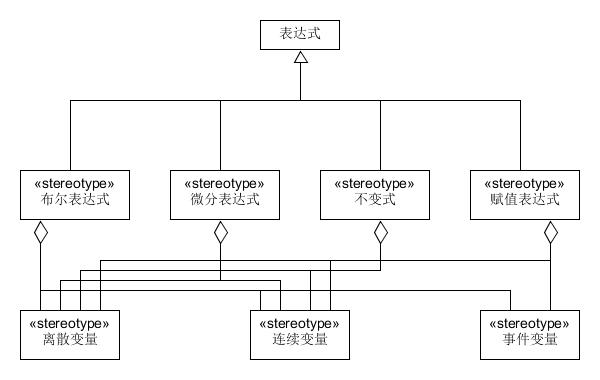
\includegraphics[width=4.8in]{expression.jpg}
	\caption{扩展的MARTE变量和表达式}
	\label{expression}
	\end{figure}
	
	\begin{myDef}布尔表达式\end{myDef}
	布尔表达式(Boolean Expression)由变量和逻辑运算符按一定语法规则组成。从最基本的层次来说,所有的布尔表达式,不论它的长短如何,其值只能是$TRUE$或$FALSE$。布尔表达式中所包含的变量可以是上述的扩展数据类型的任意一种。
	\begin{equation}
	\phi_{bol}::=A(x) \,|\, \phi_{1}\bowtie\phi_{2} \,|\, \neg\phi \,|\, \phi_{1}\vee\phi_{2} \,|\, \phi_{1}\wedge\phi_{2} \,|\, \forall x \cdot \phi(x) \,|\, \exists x \cdot \phi(x)
	\end{equation}

	\begin{itemize}
	\item $A(x)$表示关于变量$x$的任意代数表达式,包括最基本的算术运算符和常用函数。
	\item $\bowtie$为关系运算符,其值可以为$<$、$\leqslant$、$==$、$\geqslant$、$>$,表示对前后两个布尔表达式$\phi_{1}$和$\phi_{2}$的比较
	\item $\neg$、$\vee$、$\wedge$为最常见的逻辑运算操作。
	\item $\forall x  \cdot \phi(x)$和$\exists x  \cdot \phi(x)$分别表示对于任意变量$x$,关于$x$的表达式$\phi(x)$均满足,存在变量变量$x$使得关于$x$的表达式$\phi(x)$满足。
	\end{itemize}
	
	\begin{myDef}微分表达式\end{myDef}
	微分的中心思想是无穷分割,对于CPES中的连续变量,为了表示其随时间流逝的变化规律,本文使用微分表达式(Differential Expression)来描述连续变量的变化规律。
	
	微分表达式可以表示为:
	\begin{equation}
	\phi_{diff}::=F(x,dx/dt)=0
	\end{equation}
	
	它的语义可以解释为:设$m(t)$为一个连续变量,当$m(t)$是微分方程$F(x,dx/dt)=0$的解时,该微分方程被满足,且连续变量在其定义域上连续变化。
	%对于一个微分方程$\Phi(x,dx/dt)=0$,若$x$是上述方程的解,则微分表达式的形式为
	%\begin{equation}
	%\phi_{diff}::=x'=a
	%\end{equation}
	%即$dx/dt=a$,其中$a$是一个实数,表示连续变量$x$在每单位时间的变化量为$a$。
	
	\begin{myDef}不变式\end{myDef}
	不变式(Invariant)表示在系统运行过程中关于某些变量的约束。例如,对于一个电梯系统,不变式$y<800$表示在电梯运行过程中载重量应当始终小于800千克。不变式的形式化定义如下:
	
	\begin{equation}
	\phi_{inv}::=A(x) \,|\, \phi_{1}\bowtie\phi_{2}
	\end{equation}
	
	其中 $A(x)$表示关于变量$x$的任意代数表达式,包括最基本的算术运算符和一些常见的函数;$\bowtie$表示关系运算符,即$<$、$\leqslant$、$\geqslant$、$>$,$=$和$\not=$。

	\begin{myDef}赋值表达式\end{myDef}
	当$x$和$a$对应的数据类型相同时,赋值表达式(Assignment Expression)
	\begin{equation}
	\phi_{assig}::=x:=a
	\end{equation}
	表示将表达式$a$的值赋给变量$x$。在系统建模中,赋值表示变量的更新,即系统中的事件对变量造成的影响。

\section{MARTE/UML模型的扩展}
	UML中的模型可分为静态视图和动态视图,静态视图用于刻画系统的拓扑结构,动态视图用于描述系统的动态行为。静态视图包括类图、构件图、部署图等,动态视图包括用例图、顺序图、活动图、状态图等,使用者可以根据需要选择合适的模型。在继承了UML多视图建模特性的基础上,本文扩展了以下MARTE/UML模型:
	\begin{itemize}
	\item 静态视图:类图
	\item 交互视图:顺序图
	\item 行为视图:状态图
	\end{itemize}
	
	类图通过描述系统中存在的类以及类之间的关系来确定系统元素,类可以实例化为顺序图中的对象;顺序图展示了系统不同部分之间的控制流,包括可能存在的消息同步机制;状态图通过状态和迁移来描述某一对象的内部行为,顺序图中对象的内部活动可以由状态图来建模。
	
	本文在类图、顺序图和状态图中添加了建模CPES所需要的能量、混成和随机信息,给出了其对应的元模型以及语法、语义的定义。
	
%\subsection{UML用例图的扩展}	
	%用例图主要用来描述“用户、需求、系统功能单元”之间的关系。它展示了一个外部用户能够观察到的系统功能模型图。帮助开发团队以一种可视化的方式理解系统的功能需求。用例图实际上并没有描述软件系统的组织结构,而是描述了形成系统体系结构的动力。
		
	%参与者(actor)是在系统之外与系统交互的某人或某事物,它代表对象的某一个方面,并不一定作为一个独立的实体存在。用例(use case)是UML中非常重要的一个概念,在整个模型驱动软件开发过程中,用例处于一个中心地位。它是对一组动作序列的抽象描述,系统执行这些动作序列,产生相应的结果。这些结果要么反馈给参与者,要么作为其他用例的参数。关系(relation)是指用例与用例之间、参与者与用例之间的联系。主题(subject)是由一组用例所描述的一个类,这个类通常是一个系统或者子系统。
	
	%本文假设一个用例对应系统的一个功能,通过用例图直观反映系统被使用的情况以及不同参与者对系统控制。另外,通过OCL语言标注的方式注明每一个用例所相关的能源类型,结合用例被使用的情况,可以定义不同能源对系统的重要性。

	%\begin{figure}[!t]
	%\centering
	%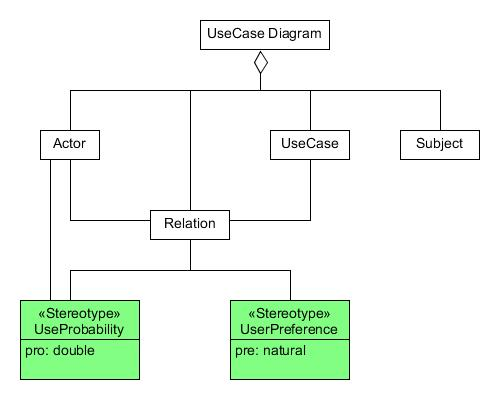
\includegraphics[width=4in]{metamodel-UD.jpg}
	%\caption{扩展的用例图元模型}
	%\label{metamodel-UD}
	%\end{figure}
	
	%ESHMARTE用例图可以用一个五元组来表示:
	
	%\begin{equation}
	%UseCase\ Diagram\ UD=<Actor, Pro, UseCase, Pref, Rel>
	%\end{equation}
	
	%其中,
	%\begin{itemize}
	%\item $Actor$是系统的所有参与者的集合,它对应于一个字符串类型的变量来唯一标识参与者的名称;
	%\item $Pro$是是概率的集合,取值范围为$[0,1]$。用例图中,概率$pro$体现在$actor$和$usecase$上,分别表示系统选择某个用户参与的概率与系统中某个用例被使用的概率。
	%\item $UseCase$代表系统中所有的用例,每个用例都必须有一个区别于其他用例的名称,其值是互不相同的字符串,也对应于一个概率$pro$代表这个用例被系统使用的概率,即$usecase=<ucname,ucpro>$。
	%\item $Pref$是参与者对用例控制的优先级的表示,为整型变量,$pref$值越小则优先级越高。
	%\item 在用例图中,关系$Rel$分为参与者与用例的关系和用例之间的关系两种。参与者和用例的关系可以用$Actor \times Pro \times Pref \rightarrow UseCase$来描述,即参与者与某个用例的关联关系中还增添了参与者使用这个用例的概率与参与者对这个用例使用的优先级。$UseCase \times UseCase \rightarrow String$可以描述用例之间的关系,用例图中涉及的关系有:关联、泛化、包含、扩展,即字符串的取值可以为以上四种之一。
	%\end{itemize}
				
	%由上述扩展的用例图的定义可知,在原有的用例图基础上,增加了随机、控制优先级和能源支持的类型三种信息。
	
	%通过在用例图中添加概率的方式,我们可以得到某个用例在系统中被使用的概率,直观反映该用例的重要程度。关于某个用例在系统中被使用的概率可以通过所有与其相关联的参与者以及参与者使用该用例的概率计算而得。对于某个用例$uc_{k}$,假设参与者$actor_{i}$使用系统的比率为$p_{a_{i}}$,在使用系统的前提下,使用用例$uc_{k}$的概率为$p_{ij}$,则得到用例$uc_{k}$被使用的概率$P_{uc_{k}}= \sum_{i=1}^N(p_{a_{i}}\times p_{ij})$($N$为所有使用用例$uc_{k}$的参与者数量)。当然,如果一个用例被使用的概率是已知的,那么直接对其进行标注即可。
	
	%\begin{figure}[!t]
	%\centering
	%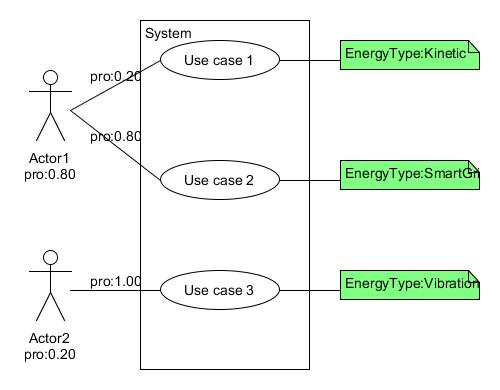
\includegraphics[width=4in]{example-UD.jpg}
	%\caption{ESHMARTE用例图示例}
	%\label{example-UD}
	%\end{figure}	
		
	%在CPES中,控制系统可能为多个参与者所使用,表现在模型中,即有多个参与者与某个用例关联。此时,$pref$的值表示了不同参与者对用例使用的优先级,值越小则优先级越高。同一个用例的所有关联的参与者的$pref$值不同。
	
	%而能源的类型可以通过OCL语言注释的形式添加在用例上。主要的的能源类型有$Vibration Energy$、$Thermal Energy$、$Kinetic Energy$、$Acoustic Energy$和$Biochemical Energy$等。
	
	%通过ESHA用例图新增的建模信息可以帮助分辨在一个多控制系统中,当对某一个控制器的控制发生矛盾时,不同参与者的优先级选择;并直观地体现出了不同用例被使用的概率,侧面反映了用例之间的重要性顺序;以及能源类型备注的方式反映了每种能源对于系统的贡献值和重要性。
\subsection{MARTE/UML类图的扩展}
	类是面向对象系统中最重要的构造块,是对一组具有相同属性、操作、关系和语义的对象的描述。类图可以帮助界定系统中的元素,是系统建模设计的基础。
	
	CPES中存在着大量能耗实体,即系统中那些运作耗能的部件,如空调、照明系统等。同时,系统中又存在一些部件,能够为系统提供能量,如太阳能电池、电网等。因此,在对CPES进行建模时,对这些实体添加合适的信息描述其对系统能量的影响是必要的。此外,一个CPES中,能量的来源可能多种多样,对能量来源进行分类标注可以帮助观测到不同能源对系统的重要性。
	
	在MARTE中,$HW\_Power$包中定义了$HW\_PowerSupply$衍型来描述能量补给,但仅仅将$HW\_Battery$作为唯一补给来源。事实上,能量的补给来源多种多样,包括热能、动能、生物能等等。在这里,对$HW\_PowerSupply$衍型进行如图\ref{harvestor}的扩展,即能量补给来源可分为:电网、太阳能、振动产能、热产能、运动产能、生化能和声波产能。
	
	\begin{figure}[!t]
	\centering
	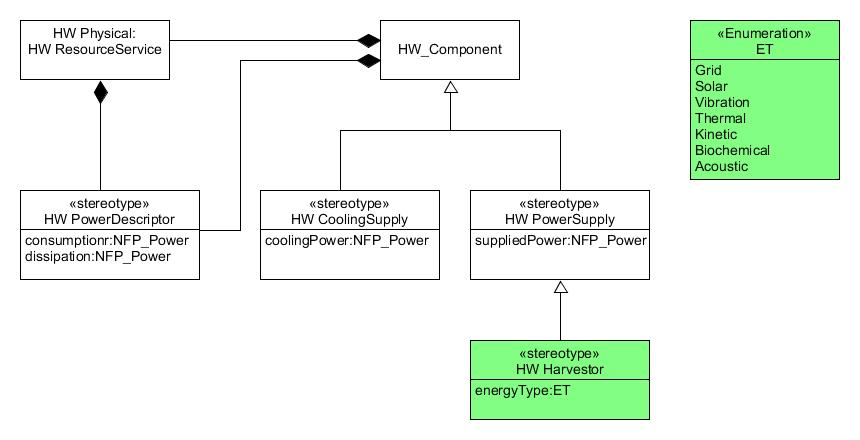
\includegraphics[width=4.2in]{harvestor.jpg}
	\caption{$HW PowerSupply$衍型的扩展}
	\label{harvestor}
	\end{figure}
	
	%在MARTE的GRM包中定义了$ResourceUsage$来描述对于资源的使用,以$energy:NFP\_Energy$的形式来描述某个类造成的能耗。结合此定义,我们将MARTE/UML类图扩展,其元模型如图\ref{metamodel-class}所示,即,对于CPES,系统中包含两类特殊衍型的对象:能量供给对象和耗能对象。
	
	扩展的MARTE/UML类图元模型如图\ref{metamodel-class}所示:1)类的属性中可以包含连续变量,用微分表达式来表示;2)类可以分为两种——耗能类和供能类。MARTE定义的$ResourceUsage$衍型可以定义耗能类,其属性包括耗能功率、工作时间和总能耗。结合上述定义的$HW Havestor$衍型,可以定义供能类,并利用$energyType$标记值来描述能量的来源。
	
	\begin{figure}[!t]
	\centering
	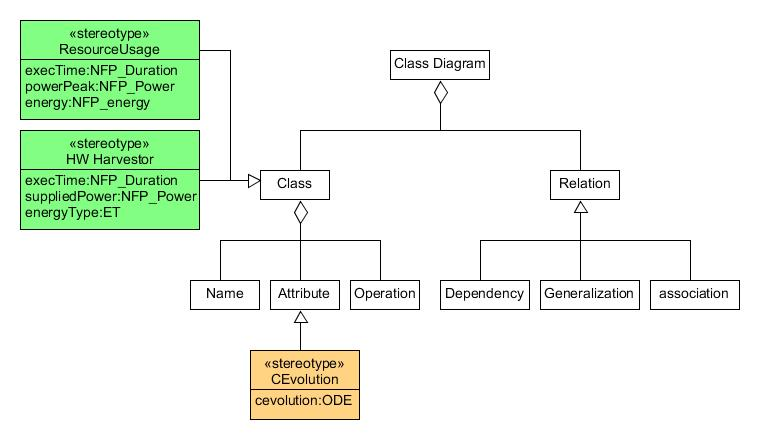
\includegraphics[width=4.8in]{metamodel-CD.jpg}
	\caption{扩展的类图元模型}
	\label{metamodel-class}
	\end{figure}
	
\subsection{MARTE/UML顺序图的扩展}	
\label{2.3.2}
	在一个待开发的系统中,任何对象都不是孤立存在的,系统中的这些对象通过消息进行交互,顺序图(Sequence Diagram)可以对系统中的交互行为进行建模,并以图形化的方式展现。

	顺序图用二维的方式来显示交互:其中,横轴代表参与交互的每个对象,纵轴表示每个对象的生命线(lifeline),即参与交互的时间。对象间的水平箭头代表它们之间消息的传递。当一个对象发送或者接收消息时,即被触活,在模型中用一个瘦高的矩形表示,被称作控制焦点(execution occurrence)。与UML1.x相比,UML2.0顺序图增加了很多可以表达各种分支、循环等情况的组合片段(combined fragments),使得顺序图建模的语义更加丰富。
	
	在CPES中,由于物理环境的开放性,不同对象之间消息的传递可能存在随机性,例如,在某个场景中,用户这个对象有一定的概率将空调度数设置得更高,也有一定概率将度数设置得更低,即在3.2.1节中定义的离散概率选择行为。除此之外,在对象的执行过程中,可能会要求系统满足某些约束,如电梯在上升的过程中要求电梯内的人不超过规定的承载量。	
	
	一个扩展的MARTE/UML顺序图可以用以下六元组表示:
	\begin{equation}
	Sequence\ Diagram\ SD=<Obj, Msg, Exec, Frag, Point, Evn>
	\end{equation}
	
	其中,
	\begin{itemize}
	\item $Obj$是有穷对象的集合,可用字符串标识对象名及其所属类名,例如:$printer:Appliance$。
	\item $Msg$是顺序图中所有消息内容的集合,它由标识符和发送对象、接受对象组成:$msg=(ctn,src,tgt)$。消息标识符$ctn$通常为$operation(parameters)$的形式,如$sendTempData(td)$表示消息内容为传递温度数据,参数为$td$。
	\item $Exec$是控制焦点的集合,表示对象执行一个动作所经历的时间段,对于每一个$exec\in Exec$对应于自己所属的对象$exec.obj\in Obj$。
	\item $Frag$是所有组合片段的集合。顺序图的各基本构成元素,可以通过组合片段封装起来,以表达不同的语义。组合片段包括:循环(loop)、分支(alt、opt)、中断(break)、临界区(critical)、并行(par)和引用(ref)等。一个$frag\in Frag$是一个三元组:$frag=(name,type,area)$,包含组合片段的名称、类型和操作域。
	\item $p \in Point$称为位点,是顺序图中所有对象生命周期上时间点的集合,代表了消息发送和接收的顺序。一个位点$p$是一个四元组:$(exec,frag,rs,order)$,其中$exec$表示位点属于哪一个控制焦点,$frag$代表位点所属的组合片段,$rs$是收发标志位,代表在该位点是接收消息还是发送消息,其取值为$\{0,1\}$,$0$代表接收消息,$1$代表发送消息。顺序图中对象的生命线并不表示精确的时间关系,但同一条生命线上的位点的先后顺序是固定的,$p.order$是位点值,其取值范围是非零自然数,代表该位点在所属对象上按时间先后顺序的排列序号。
	\item 对于每个消息$m\in Msg$,与两个事件相关联:消息的发送事件$!m$和消息的接收事件$?m$。$!m$和$?m$为同步事件。$Evn$为顺序图中所有消息事件的集合。一个消息事件$evn$包含消息内容和消息所处的位点:$evn=(msg,p)$,位点的收发标志位决定该消息事件的类型。即根据消息事件$evn$的位点的标志位$evn.p.rs$的值,可以将消息事件划分为发送消息事件$SE$和接收消息事件$RE$,且$SE \cap RE = \emptyset$。
	\end{itemize}
	
	下面,重点解释顺序图中消息事件执行顺序和组合片段的含义。
	
	\textbf{消息事件执行顺序}:顺序图中对象的生命线并不表示精确的时间,不同对象间的消息事件执行的时间顺序无法比较,但同一个对象生命线上的消息事件存在事件执行的先后顺序,因此,消息事件的执行顺序默认为偏序关系,也就是弱序列。这种弱序列关系的具体含义是:1)消息执行的最终结果是不可改变的;2)同一生命线上的不同消息事件按照先后顺序依次发生;3)不同生命线上的不同消息事件的发生顺序无法确定。
	
	\textbf{组合片段}:在图形中,组合片段表示为一个生命线上的矩形区域,其左上角有一个小五边形,其中的文字被称作标签,表示组合片段的类型。UML2.0顺序图中定义了12种组合片段,下面对常用的几种组合片段作出解释:
	\begin{itemize}
	\item 可选执行:标签为$opt$。用一个方括号括起来的布尔表达式表示进入$opt$组合片段的监护条件,当布尔表达式为真时,执行组合片段内的消息交互内容。
	\item 条件执行:标签为$alt$。组合片段内部用虚线分割成几个区域,每个区域有自己的执行监护条件,这些监护条件的交集为空。若所有监护条件均不满足,则不执行组合片段,否则执行监护条件满足的那一个区域。
	\item 并行执行:标签为$par$。同样使用虚线把组合片段内部划分为几个分区,每个分区表示一个并发执行。当进入组合片段时,同时执行所有分区,但每个分区内部的消息序列是顺序执行的,而不同分区的消息执行则存在交替的关系。这种并行执行的方式在现实生活中很常见。
	\item 循环执行:标签为$loop$。在组合片段内部区域中,设置执行的监护条件,若条件满足,则循环执行$loop$中的序列,不满足则跳出。在标签中还可以设置区间参数来表示循环执行的最少和最多次数。如$loop(1,10)$表示最少执行1次,最多执行10次。
	\end{itemize}
	
	扩展的顺序图元模型如图\ref{metamodel-sequence}所示,下面对MARTE/UML顺序图中扩展部分作出具体阐述。
	
	\begin{figure}[!t]
	\centering
	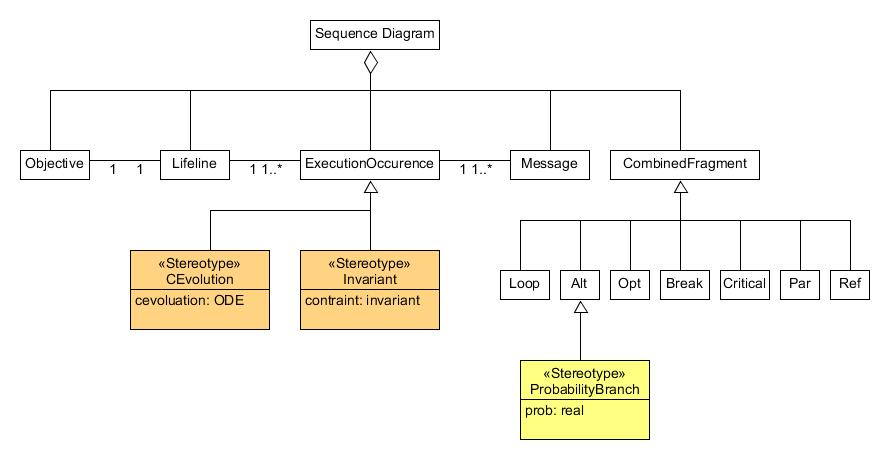
\includegraphics[width=5in]{metamodel-SD.jpg}
	\caption{扩展的顺序图元模型}
	\label{metamodel-sequence}
	\end{figure}
	
	在CPES中,离散概率选择随机行为普遍存在,对$alt$操作符进行扩展可以使其描述这种随机行为——即不同分区的选择不是由监护条件决定,而是由每一分区的执行概率决定。系统执行哪一个分区是不确定的,按照概率随机选择。每一个分区$area_{i}$对应于一个取值为$[0,1]$的$prob_{i}$表示该分区被选择的概率。如图\ref{example-SD}所示,在对象$a$发送消息时,有$80\%$的概率发送正确的消息$sendRight(rData)$,$20\%$的概率发送错误消息$sendWrong(wData)$。
	
	\begin{figure}[!t]
	\centering
	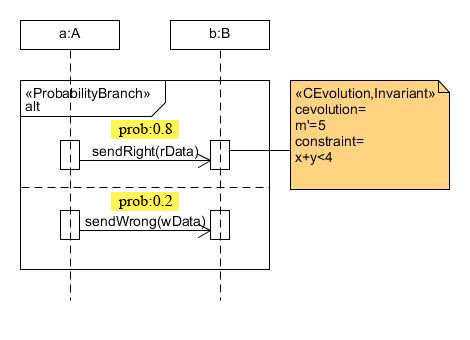
\includegraphics[width=3in]{example-SD.jpg}
	\caption{扩展的顺序图示例}
	\label{example-SD}
	\end{figure}	
	
	CPES是一个混成系统,在某个对象处于执行阶段时,系统可能会存在某些特定的约束,或者某些连续变量的变化率可能维持不变。在对象的控制焦点上,可以通过添加不变式和微分表达式来描述这些信息。如图\ref{example-SD}所示,在对象$b$的第一个控制焦点执行过程中,连续变量$m$的变化率始终为$5$,且变量$x$和$y$之和始终小于4。
	%操作语义的基本思想是用抽象的方法描述语言中每一成分的执行效果,以免所描述的语义依赖于该语言实现时所用的具体计算机,其突出特点在于具有直观的表述方式。
	
	消息事件是顺序图中的重要元素,消息的执行即代表了顺序图的动态逻辑语义。下面结合3.2.2节中定义的事件执行顺序,使用逻辑推导的方式来形式化定义顺序图中\textbf{消息事件执行顺序}的含义:
	\begin{itemize}
	\item $evn_{x}.p.exec.obj==evn_{y}.p.exec.obj \wedge evn_{x}.p.order<(>)evn_{y}.p.order \Longrightarrow evn_{x} \prec(\succ) evn_{y}$
	
	如果消息事件$evn_{x}$和$evn_{y}$的位点同属于一个对象,且$evn_{x}$的位点值小于(大于)$evn_{y}$,则消息事件$evn_{x}$先于(晚于)$evn_{y}$发生。
	\item $evn_{x}.msg==evn_{y}.msg \wedge evn_{x}.p.rs \oplus evn_{y}.p.rs \Longrightarrow evn_{x} \approx evn_{y}$
	
	如果消息事件$evn_{x}$与$evn_{y}$所包含的消息内容相同,且消息对应的位点收发位相异,即一个为消息发送事件,一个为对应的消息接收事件,则$evn_{x}$和$evn_{x}$同时发生。
	\item $\neg (evn_{x}.p.exec.obj==evn_{y}.p.exec.obj) \Longrightarrow evn_{x} \sim evn_{y}$
	
	如果消息事件$evn_{x}$与$evn_{y}$不属于同一个对象,则它们的执行顺序不可判定。
	\end{itemize}
	
	消息事件执行顺序比较的是单个消息事件之间的时间先后顺序。而\textbf{消息事件执行序列}是相对于整个顺序图而言的,它将消息事件按照执行顺序依次排列,并用逗号隔开(本文定义的消息事件是同步事件,执行序列里可以仅列出所有发送事件或所有接收事件),形如:$ES=\{evn_{1},evn_{2},... \}$。

	一个顺序图的消息执行序列是不确定的,原因如下:1)不同生命线上消息的执行顺序不能确定;2)组合片段$opt$、$alt$中消息执行的不同选择让消息事件执行序列的结果具有不确定性,使得顺序图产生语义分歧。下面,针对$opt$和$alt$操作符对消息事件执行序列的影响作出形式化解释:
	
	\begin{itemize}
	\item $evn_{x}.p.frg.type==opt \Longrightarrow  \{ ES_{1},evn_{x},ES_{2} \} | \{ ES_{1},ES_{2} \} $
	
	如果消息事件$evn_{x}$属于一个$opt$组合片段,设$ES_{1}$是$opt$组合片段之前的消息执行序列,$ES_{2}$是$opt$组合片段之后的消息执行序列。由于条件满足时,$opt$操作域内的消息事件才会被执行,所以顺序图的消息执行序列为$\{ ES_{1},evn_{x},ES_{2} \} $或者$\{ ES_{1},ES_{2} \}$。
	\item $evn_{x}.p.frg.type==alt \wedge evn_{y}.p.frg.type==alt \wedge evn_{x}.p.frg.name==evn_{y}.p.frg.name \Longrightarrow \{ ES_{1},evn_{x},ES_{2} \} | \{ ES_{1},evn_{y},ES_{2} \}$
	
	如果消息事件$evn_{x}$和$evn_{y}$同属于一个$alt$组合片段,设$ES_{1}$是$alt$组合片段之前的消息执行序列,$ES_{2}$是$alt$组合片段之后的消息执行序列。由于$alt$选择的互斥性,则顺序图的消息执行序列为$\{ ES_{1},evn_{x},ES_{2} \}$或$\{ ES_{1},evn_{y},ES_{2} \}$。
	\item $evn_{x}.p.frg.type==alt \wedge evn_{y}.p.frg.type==alt \wedge evn_{x}.p.frg.name==evn_{y}.p.frg.name \wedge evn_{x}.p.frg.area.prob==p_{1} \wedge evn_{y}.p.frg.area.prob==p_{2} \Longrightarrow \{ ES_{1},evn_{x},ES_{2} \}_{p_{1}} | \{ ES_{1},evn_{y},ES_{2}\}_{p_{2}} $
	
	如果消息事件$evn_{x}$和$evn_{y}$同属于一个$alt$组合片段设$ES_{1}$是$alt$组合片段之前的消息执行序列,$ES_{2}$是$alt$组合片段之后的消息执行序列。由于$alt$选择的互斥性,则顺序图的消息执行序列有$p_{1}$的可能性为$\{ ES_{1},evn_{x},ES_{2} \}$,$p2$的可能性为$\{ ES_{1},evn_{y},ES_{2} \}$。
	\end{itemize}
	上述推导过程考虑的是单个事件的情形,对于可选片段区域中包含多个事件的情形,所得消息执行序列的结果是类似的。
	
\subsection{MARTE/UML状态图的扩展}
\label{2.3.3}
	顺序图提供了控制流随时间推移的可视化轨迹,但它无法表现单个对象内部的状态变化。而在系统的建模、设计中,这些动态细节的刻画是必需的。因此,需要状态图来对单个对象的生命周期进行描述。
	
	状态图(State Chart)用来表示一个对象在它的生命周期中对外部事件的响应、状态的变化、生命周期的变迁,以及对过去行为的依赖。它将对象与其外部世界分离开来,从局部视角出发,独立考察其行为。
	
	一个扩展的MARTE/UML状态图定义如下:
	\begin{equation}
	State\ Chart\ SC=(State, s_{0}, Inv, Diff, Distr, \tau, Evn, Grd, Prob, Act,Eng)
	\end{equation}
	
	其中,
	\begin{itemize}
	\item $State$为研究对象所有状态的集合。
	\item $s_{0}$为初始状态。
	\item $Inv$代表所有状态上的约束,以不变式的形式描述。
	\item $Diff$是微分表达式的集合,描述了在某个状态下连续变量随时间变化的速率。
	\item $Distr$是时延概率分布,描述了在某个状态下每个时刻发生迁移的概率。
	\item $\tau$是从一个状态到另一个状态的迁移的集合。
	\item $Evn$是所有触发事件的集合,UML中允许没有触发事件的迁移,被称作完成迁移。
	\item $Grd$为所有监护条件的集合,以布尔表达式的形式描述。
	\item $Prob$对应于$[ 0,1 ]$上的实数,代表概率值。
	\item $Act$是迁移发生后带来的效应,通常由赋值表达式组成。
	\item $Eng$表示系统的能耗函数,根据能耗在状态图中产生的位置不同,可以分为:$S \rightarrow R$和$\tau \rightarrow R$两种。能耗值为正代表系统消耗能量,为负代表系统产生能量。
	\end{itemize}
	
	状态和迁移是状态图中最重要的两个元素,下面分别对它们进行更为详细的解释。
	
	\emph{状态}:对于每一个$s \in State$,有$s = (sname,\phi_{inv},\phi_{diff},\phi_{distr}, \phi_{eng})$,其意义是:对于一个系统状态$s$,具有唯一的字符串型状态名$sname$,且在该状态下,系统中的连续变量的变化率满足$\phi_{diff}$。同时,系统变量满足约束$\phi_{inv}$,当$\phi_{inv}$违背且迁移尚未发生时,系统进入终止状态。$\phi_{distr}$为状态的迁移赋予了随机的特性,即系统在状态$s$停留多久取决于时延概率分布$\phi_{distr}$,它定义了系统在每一个时间点发生迁移的概率,即刻画了时延随机行为。$\phi_{eng}$是能量的微分表达式,定义了在状态$s$上能量的变化率。
	
	\emph{迁移}:$\tau:State \times Evn \times Grd \times Prob \times Act \times Eng \rightarrow State$。即迁移是系统由一个源状态$src$向目标状态$tgt$的转变。在触发事件发生的情况下,迁移必须满足一定的监护条件才能发生。$prob\in[0,1]$定义了迁移从源状态到某个目标状态的概率值,对于状态$s$,在相同的触发事件和监护条件下,若其对应于$N$个目标状态,则其到所有目标状态的概率之和为1,即$\sum_{i=1}^N prob_{i} =1$。若在某触发事件和监护条件下,不存在概率分支情况,则迁移是确定的。$Eng:\tau \rightarrow R$定义了迁移$\tau$造成的能耗。
	
	图\ref{metamodel-SC}为扩展状态图的元模型,通过元模型,可以更直观地体现本文所做的扩展:
	\begin{figure}[!t]
	\centering
	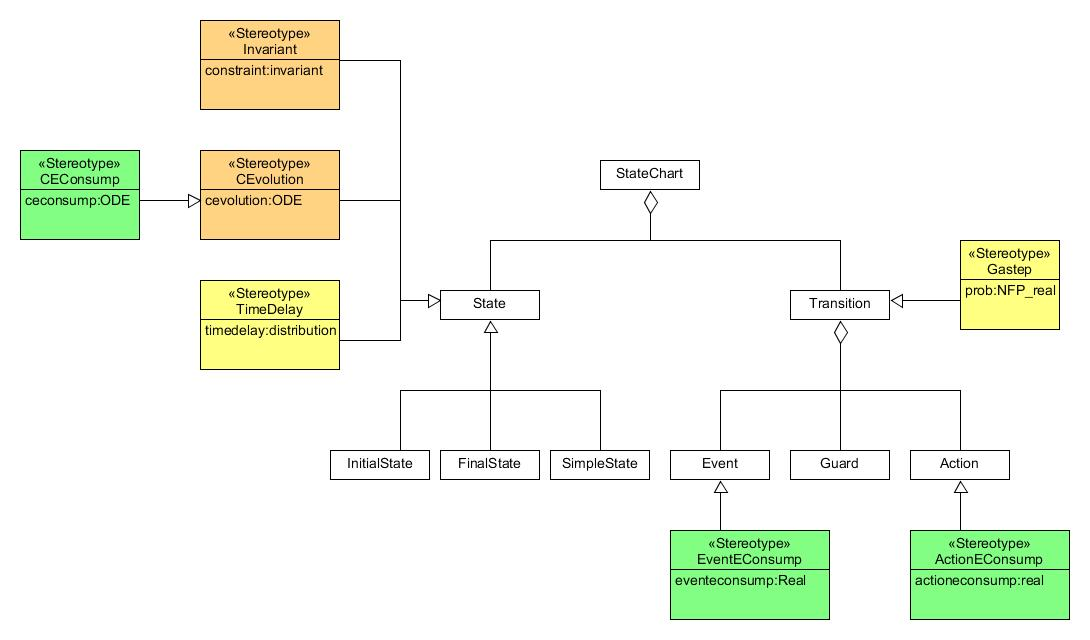
\includegraphics[width=6in]{metamodel-SC.jpg}
	\caption{扩展的状态图元模型}
	\label{metamodel-SC}
	\end{figure}	
	
	\begin{itemize}
	\item 针对CPES的混成特性,对状态增加了$CEvolution$衍型,用微分表达式来刻画系统中连续变量随时间的变化速率;
	\item 针对CPES中存在的两种随机行为,在状态上添加了$TimeDelay$衍型,并使用时延概率分布来描述时延随机行为;而迁移上则利用MARTE原有的$Gastep$衍型刻画了离散概率选择行为;
	\item 在状态图中,根据产生的位置不同可将能耗分为两类:1)在状态上产生的能耗,此时能量是以连续变量的形式通过微分表达式来定义其随时间变化的速率,并结合实际在状态上的停留时间计算而得;2)在迁移上产生的能耗,迁移的触发事件和动作事件的执行可能伴随能量的产生与消耗,与状态上的能量不同,迁移是不耗时的,因此用一个离散的实数值来记录迁移造成的能耗。
	\end{itemize}
	
	图\ref{example-SC}为扩展的MARTE/UML状态图的简单示例,其中,$state1$为$CEvolution$衍型的状态,在该状态下,连续变量$s$随时间的变化率为2,;$state1$在$event$事件的触发下,有$80\%$的可能性迁移至$state2$状态,$20\%$的可能性迁移至$state3$状态,同时,$event$事件会带来两个单位的能耗;在$state2$状态下,系统每单位时间耗能为5,在$state3$状态下,系统每单位时间耗能为10。
	%此处的示例没有列举出所有扩充的信息,在第五章会结合具体案例展现扩展的MARTE/UML的使用。
	
	\begin{figure}[!t]
	\centering
	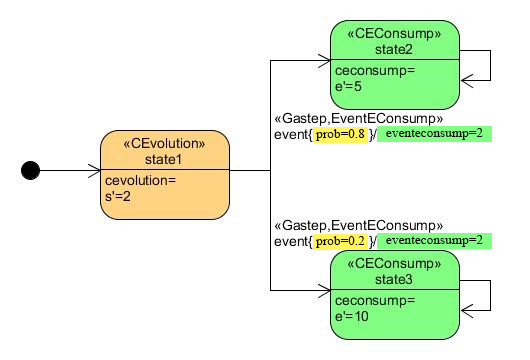
\includegraphics[width=3.5in]{example-SC.jpg}
	\caption{扩展的状态图示例}
	\label{example-SC}
	\end{figure}
	
	同样地,为了准确定义状态图的动态语义,这里使用逻辑推导规则对状态图中的两种迁移作出语义解释。
	
	顺序图中的主要对象是消息事件,其动态逻辑语义可以由消息执行序列表示,而状态图中最重要的元素是状态和迁移,由于本文定义的迁移已经包含了对应的源状态和目标状态的信息,因此,迁移序列$TS=\{ \tau_{1},\tau_{2},...  \}$即可描述状态图由初始状态发生迁移、逐步演化的过程。对于一个状态图而言,由于离散概率选择和状态上时延概率分布的存在,迁移序列是不确定的。
	
	\begin{itemize}
	\item 离散迁移:
	
	$ \tau_{i}.src==\tau_{j}.src \wedge \tau_{i}.evn==\tau_{j}.evn \wedge \tau_{i}.evn==1 \wedge \tau_{i}.grd==\tau_{j}.grd \wedge \phi_{grd_{i}}==TRUE \Longrightarrow \{ TS_{1},\tau_{i}... \}_{\tau_{i}.prob} | \{ TS_{1},\tau_{j}... \}_{\tau_{j}.prob}$ 
	
	设$TS_{1}$为$\tau_{i}$之前的迁移序列,当迁移$\tau_{i}$和$\tau_{j}$所对应的源状态、触发事件和监护条件均相同,且触发事件发生、监护条件满足时,它们被触发的概率由各自的迁移概率值$prob$决定,即系统的迁移序列有$\tau_{i}.prob$的概率为$\{ TS_{1},\tau_{i}... \}$,有$\tau_{j}.prob$的概率为$\{ TS_{1},\tau_{j}... \}$。对于包含多个概率选择的迁移情况,结果类似。
	\item 时延概率迁移:
	
	上述离散迁移仅仅考虑了迁移的概率选择对系统迁移序列的影响,并没有考虑状态上时间延迟的随机性。$\tau_{i\_c_{i}}$表示迁移$\tau_{i}$在其源状态$\tau_{i}.rs$上停留的时间为$c_{i}$。
	设$TS_{1\_C_{1}}$为$\tau_{i}$之前的迁移序列,即系统执行迁移序列$TS_{1}$的耗时为$C_{1}$,则$\{TS_{1\_C_{1}},\tau_{i\_c_{1}}...\}_{\tau_{i}.rs.\phi_{distr}(c_{1})} | ... | \{TS_{1\_C_{1}},\tau_{i\_c_{i}}...\}_{\tau_{i}.rs.\phi_{distr}(c_{i})}$表示对应的时延概率迁移序列。
	\end{itemize}
	
\section{本章小结}
	UML是最常用的系统建模语言之一,MARTE是针对实时嵌入式系统的UML profile,MARTE/UML模型提供了强大的实时性、嵌入式方面的建模能力。但对于智能建筑等CPES的混成、随机和能量感知特性,MARTE/UML建模方式仍然存在一定的局限性。针对此问题,本章首先定义了CPES中的两种随机行为;接着给出了MARTE元素的扩展,包括数据类型和表达式;最后结合MARTE,扩展了UML的类图、顺序图和状态图,给出了其元模型和语法语义,以支持CPES系统的建模。本章给出了扩展模型的简单示例,关于扩展模型的实际应用,可参考第五章案例部分。
	




\chapter{能耗随机混成自动机的验证}
\label{ch4}
\vspace{-0.7cm}
	MARTE/UML采用多视图的方式对系统进行设计、描述,但由于其半形式化的特性,无法实现模型的定性、定量验证。自动机不仅可以刻画系统的行为,且目前已存在很多基于自动机的模型检测方法。本章首先基于随机混成自动机的概念,给出了能耗随机混成自动机的形式化语法和语义,支持显式建模系统中能量的产生与消耗。接着,提出了从MARTE/UML状态图到能耗随机混成自动机的映射规则和转换算法,实现了不可执行模型到到可执行模型的自动转换。最后,基于我们的建模、仿真、验证平台Modana\citep{DBLP:conf/compsac/ChengWLD15,杜德慧2017一种面向}和模型验证工具UPPAAL-SMC\citep{DBLP:journals/spe/BehrmannDLPY11,DBLP:journals/corr/abs-1207-1272},给出了本文所提的智能建筑能耗建模与分析方法的实现框架。
	
\section{能耗随机混成自动机}
\subsection{ESHA的语法}
	随机混成自动机(Stochastic Hybrid Automata,SHA)\citep{Hu2000Towards,David2011Statistical,程贝2016基于抽象和学习的统计模型检测研究}可以被视作添加了随机语义扩展后的混成自动机(Hybrid Automata)\citep{Henzinger1996The}。根据SHA的定义,系统可以由位置(location)和位置间的迁移(transition)描述。在每一个位置上,连续变量随时间的变化速率可能不同,每次迁移可能伴随着系统变量的重新赋值(valuation)。SHA具有混成的语义:在位置上可以利用速率向量(rate vector)来定义连续变量随时钟的变化率;而在位置间的迁移过程中,可以对变量进行重新赋值;同时,SHA也具有随机的语义:位置上可以用时延函数来描述系统在该位置时间延迟的概率;位置之间的迁移可以定义离散的概率值来表示从某个位置发生某个迁移的特定概率。
	
	为了能够显式地描述CPES中的能耗变化,我们在SHA上添加能耗的信息,并且针对能耗产生的不同方式,进行了分类。能耗随机混成自动机的定义如下:
	\begin{myDef}能耗随机混成自动机\end{myDef}	
	一个\textbf{能耗随机混成自动机}(Energy Stochastic Hybrid Automata,ESHA)是一个九元组$ESHA = (L,l_{0},X,\Sigma,T,R,I,F,E)$。
	\begin{itemize}
	\item $L$是位置的有限集合;
	\item $l_{0} \in L$代表初始位置;
	\item $X$是所有变量的集合,包括离散变量、连续变量以及时钟,且时钟的取值范围为 $\mathbb{R^{+}}$;
	\item $\Sigma = \Sigma_{i} \cup \Sigma_{o} $是动作的有限集合,分为输入动作($\Sigma_{i}$)和输出动作($\Sigma_{o}$);
	\item $T \subseteq L \times \Phi(X) \times Prob \times \Sigma \times 2^{X} \times L$是迁移的有限集合,即一个从 $l$ 到 $l^{'}$ 的迁移在输入动作和变量的约束条件下以一定的离散概率发生,并伴随着输出动作和变量的重新赋值;
	\item $R:L\rightarrow \mathbb{N}^X$为每一个位置赋予了一个速率向量来刻画在该位置上连续变量的变化率;
	\item $I : L \rightarrow Inv$ ,其中$Inv$描述了ESHA中位置上的变量约束, $I$定义了这种映射关系;
	\item 对于每一个位置$l \in L$,$f(l)$为该位置上的时延函数。
	\item $E:T \cup L \rightarrow \mathbb{R}$代表ESHA所描述的动态行为过程中的能耗,它将自动机中的每个位置和每条迁移映射到一个实数,来记录相应的能耗,即
	\begin{equation}
	E = E_{t} \cup E_{l}
	\end{equation}
	其中,$E_{t}:T \rightarrow \mathbb{R}$将每个迁移映射到实数上,表示迁移带来的能耗;$E_{l}:L \rightarrow \mathbb{R}$将每个位置映射到实数上,以记录在位置上产生的能耗。迁移和位置上的能耗值均可正可负,能耗值为正代表系统消耗能量,为负代表系统产生能量。
	\end{itemize}
	
\subsection{ESHA的语义}
	SHA的语义可以用一个标签迁移系统描述,在解释ESHA的语义之前,先介绍如下定义。

	\begin{myDef}标签迁移系统\end{myDef}
	一个\textbf{标签迁移系统}(Labeled Transition System,LTS)\citep{DBLP:journals/fm/Trybulec09}是这样一种结构: $\langle S, A, \longrightarrow\rangle$ 
,集合$S$包含系统所有的状态, 集合$A$包含所有标签, 迁移关系 $\longrightarrow\,\subseteq S\times A\times S$。$(s,a,s')\in\longrightarrow$通常表示为$s\stackrel{a}{\longrightarrow}s'$ 。
	
	时钟标签迁移系统是一种标签为时钟集合的标签迁移系统。对于每一个状态,最多有$2^n$条对外的迁移,其中,$n=|C|$表示时钟的数目。每个迁移都可能伴随着时钟的重置。
%A special state, denoted $\bot$, stands for a sink state where the constraint is violated.

	\begin{myDef}时钟标签迁移系统\end{myDef}
	一个\textbf{时钟标签迁移系统}(Clock-labelled Transition System,CLTS)是这样一种结构: $\langle S, C, \longrightarrow\rangle$,其中$\langle S, 2^C, \longrightarrow\rangle$ 是一个标签迁移系统。

	%为了能够建模系统中的能耗,我们通过在每一个位置和迁移上加能耗标注进一步扩展了时钟标签迁移系统,这个扩展后的结构被称作\textbf{能耗时钟标签迁移系统}。
	
	\begin{myDef}能耗随机时钟标签迁移系统\end{myDef}
	基于CLTS,在\citep{DBLP:conf/facs2/DuHJMY16}中我们定义了Probabilistic CLTS的概念,进一步地,可以扩充定义能耗随机时钟标签迁移系统(Energy Stochastic Clock-labelled Transition System,ESCLTS)。ESCLTS是一个特殊的时钟标签迁移系统,其中,$\longrightarrow\ \subseteq (S \cup F \cup E_{l}) \times 2^C \times Prob \times E_t \times (S \cup F \cup E_{l})$。
	
	$F$表示状态$S$处的时延函数,即描述了状态$S$处迁移发生与时间的概率分布关系;$Prob \subseteq \mathbb{R}$是一个[0,1]上的实数,对于一个给定的迁移$t=(s \cup f \cup e_{l},\Gamma,prob,e_{t},s' \cup f' \cup e_{l}^{'})$,$\pi(t)=prob$表示此迁移被触发的概率为$prob$。
	$E_{t(l)}$ 中的元素$e_{t(l)}$代表了某个特定迁移(位置)产生的具体能耗数值。$e_{t(l)}>0$代表系统消耗了能量, $e_{t(l)}<0$代表系统产生了能量。
%type/update

	\begin{myDef}迁移能耗\end{myDef}
\emph{迁移能耗}代表自动机在进行位置迁移时,随之产生的能耗。它由一个三元组来表示:$E_{t} = (Type, Update, \lambda)$,其中,$Type$和$Update$分别表示迁移触发的原因和迁移触发后的后果(包括对系统某些变量的改变)。

	\begin{itemize}
	\item $Type ::= sync | guard$,其中, $sync$ 表示自动机与另一个自动机之间存在消息交互,即由消息触发了迁移;$guard$表示迁移的触发仅仅是由于某个位置上不变式约束条件的违背而造成的。
	\item $Update ::= true | false$ , $true$代表此迁移造成了系统某些变量的重新赋值,而$false$意味着不改变系统的任何变量。
	\end{itemize}

	现在,我们给出$\lambda$的定义,它是系统某次迁移产生的能耗的计算值—— $\lambda:Type \cup Update\rightarrow\mathbb{R}$。在$Type$和$Update$值的不同组合下,$\lambda$的值将有四种计算方式,具体规则如表\ref{energy-transition}所示。

	\begin{table}[!t]
	\renewcommand{\arraystretch}{1.4}
	\caption{迁移能耗的计算}
	\label{迁移能耗的计算}
	\centering
	\begin{tabular}{c c c}
	\hline
	Type & Update & $\lambda$ \\
	\hline
	sync & true & $e_{t}.sync + e_{t}(update)$\\
	sync & false & $e_{t}.sync$\\
	guard & true & $e_{t}(update)$\\
	guard & false & $0$\\
	\hline
	\label{energy-transition}
	\end{tabular}
	\end{table}
 
	根据迁移触发原因的不同,我们来分析ESHA中不同类型迁移所带来的能耗。现实世界中系统不同模块间的信息传递在自动机中被建模为模型间的同步信号。对于特定环境下的系统而言,这种信息传输产生的能耗由线路的物理特性和系统的消息传递机制决定,而与消息的内容无关。因此,可以将每次消息传输的能耗视作一个固定值,记作$e_{t}.sync$。值得注意的是,在ESHA中,一次消息传递被建模为一个模块的信号接收事件和另一个模块的信号发送事件,为了避免能耗的重复计算,可以限定只计算发送事件能耗或只计算接收事件能耗。
	由于不变式条件的违背而产生的迁移,仅仅代表了系统中某些变量值的演化触发了系统的状态迁移,并没有实际动作发生,因此不会带来任何能耗。

	迁移上的$Update$代表对系统中某些变量的赋值,在实际中,这往往意味着系统需要采取一些措施来改变某些变量的值。例如,在一个汽车系统中,``$acceleration =  acceleration +2$''意味着汽车引擎需要加大马力来使得加速度增加两个单位,这一动作会带来额外的能耗。另外,在某些时刻,系统可能需要补充能量,如利用太阳能产生能量,能耗值为负即表示能量的补给。迁移上的赋值操作带来能耗值由具体的动作所决定,故记作$e_{t}(update)$。值得一提的是,在对CPES建模时,由于系统的实时性,常使用时钟来控制某些事件的发生。迁移上可能会伴随着时钟的重置,这实际上是为了建模系统控制而人为设定的,并不耗能。
	
	正如表\ref{迁移能耗的计算}所呈现的,一个离散迁移所产生的能耗为触发事件执行的能耗和动作效应的能耗之和。 对于一个能耗随机时钟标签迁移系统 $\langle S \cup F \cup E_l, 2^{C} \cup E_t, \longrightarrow\rangle$,我们把$e_{t}(t)=e_{t}.\lambda$叫作离散迁移$t \in \longrightarrow$的能耗值。  

\begin{myDef}位置累积能耗\end{myDef}
	位置之间的迁移表示的是系统的离散行为,然而,由于时间的流逝以及系统处于不同位置时能量随时间的变化速率不同,在系统的不同位置,会累积特定的能耗,这种在位置上产生的能耗被称作\textbf{位置累积能耗}。

	位置累积能耗可以通过公式$e_{l}(l) =\int r(t) dt$, s.t. $(l,T)\rightarrow(l,T + \Delta T)$计算而得,其中,$\Delta T$代表了时间流逝的长度,$r(t)$代表在某个位置上能耗随时间的变化率,$(l,T)\rightarrow(l,T + \Delta T)$意味着在某个位置上停留的时间必须使得系统变量满足该位置上的不变式约束。

\begin{myDef}能耗链\end{myDef}
	一条从位置$loc_{1}$到位置$loc_{n}$的能耗链是由位置和迁移的交替排列组成的有向序列,$\gamma = loc_{1,\Delta T_{1}} \xrightarrow{t1} loc_{2,\Delta T_{2}} \xrightarrow{t2} ... \xrightarrow{t(n-1)} loc_{n,\Delta T_{n}}$。尤其需要注意序列的方向,$loc_{1} \xrightarrow{t_{x}} loc_{2}$和$loc_{2} \xrightarrow{t_{y}} loc_{1}$是不同的,因为迁移具有方向性,且不同的迁移带来的能耗不同。一条能耗链的总能耗值是所有迁移能耗和位置累积能耗之和,即
	\begin{equation}
	E(\gamma) = \sum_{i=1}^{n-1}e_{t_{i}}.\lambda + \sum_{i=1}^{n} \int r(t) dt
	\end{equation}
	
	\textbf{最小迁移能耗链}:从位置$loc_{1}$到位置$loc_{n}$通常具有不止一条迁移能耗链,其中,能耗值最小的被称作最小迁移能耗链,即 $\forall \gamma_{l_{1} \rightarrow l_{n}}, E(\gamma_{l_{1} \rightarrow l_{n}}^{min})\leq E(\gamma_{l_{1} \rightarrow l_{n}})$。
		
\section{MARTE模型到ESHA的转换}
	MARTE/UML类图定义了系统的静态元素;顺序图描述了系统为实现某个功能,不同对象之间的交互关系;状态图则更详尽地刻画了对象内部发生的状态变化。状态图与随机混成自动机本质上描述的都是单个对象的动态变化过程,因此,可以基于语义将扩展的MARTE/UML状态图的元素映射为ESHA的元素,实现设计模型到可执行模型的转换,进而对转化得到的模型实现仿真和验证。

\subsection{模型映射规则}
	\textbf{转换的依据}
	
	从建模的基本思想来说,模型是对现实世界的抽象。针对同一个系统,观察的角度和重点不同以及建模的方法不同,都会得到不同的系统模型。但是,当关注的角度相同、针对同样的性质时,不同的建模方法构建出来的系统模型只是表达方式上存在差异,本质上其逻辑语义是一致的\citep{彭大天2013基于}。
	
	\textbf{元素的映射}
	
	根据前述对扩展的MARTE/UML状态图和ESHA的定义,我们给出了如图\ref{SC2ESHA}所示的元素映射规则,其中,ESHA以UPPAAL-SMC工具中的图形化形式表示。UPPAAL-SMC是一个常用的统计模型检测工具,其理论基础是随机混成自动机。本文定义的ESHA可以视作SHA添加了能耗的扩展版本,我们通过自定义特定变量来表示迁移能耗和位置累积能耗。此外,在UPPAAL-SMC中,离散概率选择迁移需要添加Branch节点,且每条迁移的触发概率以比值$Probability Weight$表示。
	
	\begin{itemize}
	\item 状态映射:初始(终止)状态对应于初始(终止)位置;$Invariant$衍型的状态,其$constraint$标记值的不变式表达式对应于位置上的不变式约束;$CEvolution$衍型的状态,其$cevolution$标记值的微分表达式对应于位置上的微分等式;$CEConsump$衍型的状态,其$ceconsump$标记值的能耗微分表达式对应于位置上的能耗微分等式;对于$TimeDelay$衍型的状态,若其$timedelay$标记值的时延概率分布为指数分布,则对应于位置上的时钟迁移约束;若时延概率分布为均匀分布,则由位置上的约束和迁移上的监护条件组合表示;
	\item 迁移映射:状态图中迁移的源状态和目标状态分别对应于ESHA中的源位置和目标位置,触发事件、监护条件,迁移概率以及执行效应也都一一对应;在状态图中,一个$EventEconsump$衍型的迁移,其触发事件的能耗在ESHA中被定义为$eventeconsump$变量的重新赋值;一个$ActionEconsump$衍型的迁移,其执行效应的能耗在ESHA中被定义为$actioneconsump$变量的重新赋值。
	\end{itemize}
	
	%扩展的MARTE/UML状态图通过状态和迁移来刻画系统中某个对象的动态性质;能耗随机混成自动机通过位置和迁移来描述对象状态的演变过程。二者的语义本质是一致的,因此,可以通过元素映射将状态图转换为ESHA。

	\begin{figure}[!b]
	\centering
	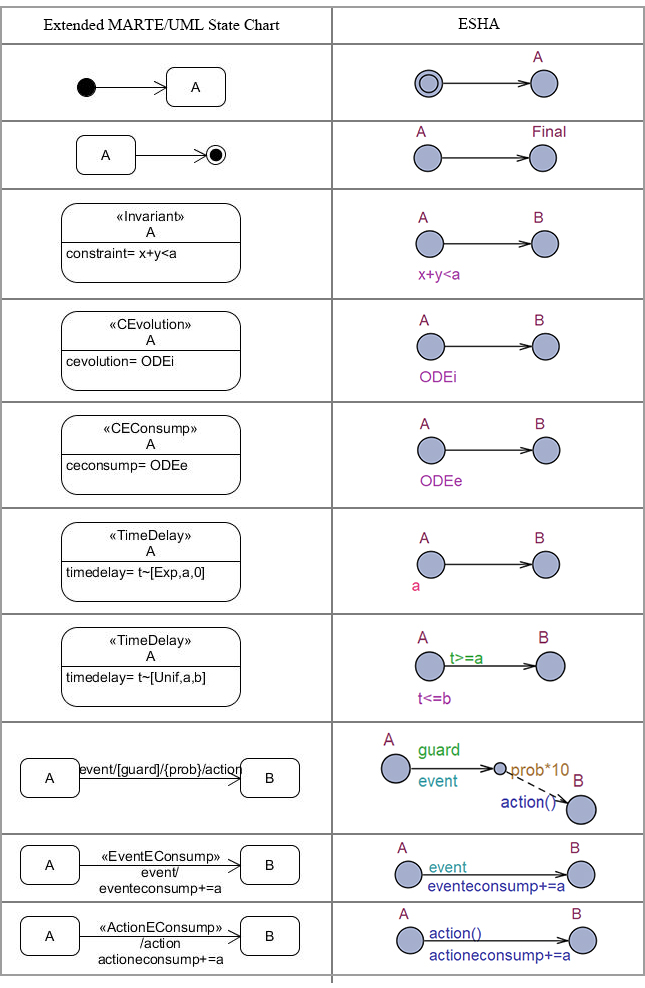
\includegraphics[width=3.7in]{mapping(new).jpg}
	\caption{扩展的MARTE/UML状态图-ESHA模型的映射规则}
	\label{SC2ESHA}
	\end{figure}
	
	由图中的映射关系可知,扩展的MARTE/UML状态图元素和ESHA模型元素在表达含义上具有一致性,为实现模型转换提供了依据。
	
	\textbf{示例}
	
	图\ref{example-trans}所示为一个简单的模型映射示例:一个加热器初始处于空闲状态,当接收到$on?$信号后,有$50\%$的概率进入$heat1$状态,$50\%$的概率进入$heat2$状态,且接收信号这一事件会产生2个单位的能耗;当加热器处在$heat1$状态时,每单位时间的能耗值为5,提供的加热功率为2,且加热4至5个单位时间后会再次返回空闲状态;当加热器处在$heat2$状态时,每单位时间的能耗值为10,提供的加热功率为5,同样地,在加热4至5个单位时间后会再次返回空闲状态。图\ref{trans-sc}为该示例对应的扩展MARTE/UML状态图,图\ref{trans-esha}为按照元素映射规则转换后的ESHA模型。
	
	\begin{figure}
	\centering
	\subfigure[扩展的MARTE/UML状态图]{
	\begin{minipage}[b]{0.4\textwidth}
	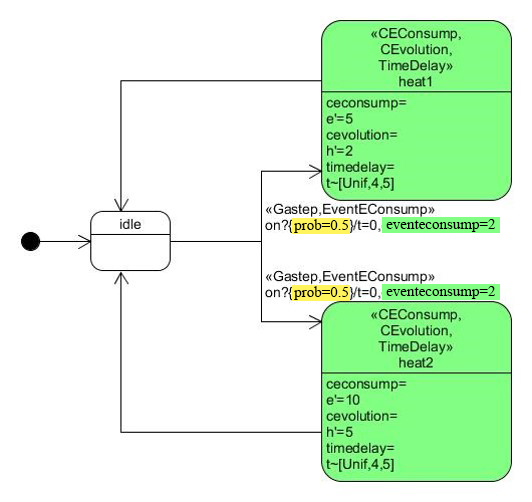
\includegraphics[width=1\textwidth]{example-trans.jpg} 
	\end{minipage}
	\label{trans-sc}
	}
	\subfigure[对应的UPPAAL-SMC ESHA模型]{
	\begin{minipage}[b]{0.4\textwidth}
	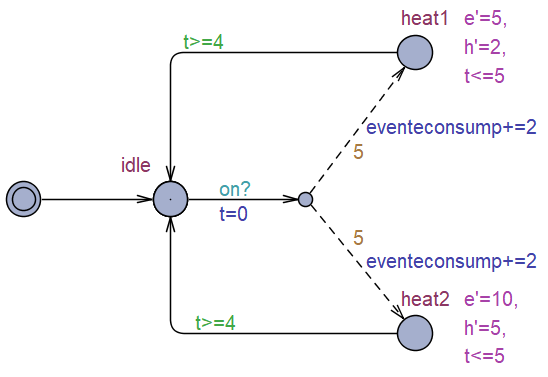
\includegraphics[width=0.8\textwidth]{example-trans.png} 
	\end{minipage}
	\label{trans-esha}
	}
	\caption{扩展的MARTE/UML状态图-ESHA模型的映射示例}
	\label{example-trans}
	\end{figure}

\subsection{模型转换伪代码}
	下面我们给出从扩展的MARTE/UML状态图到UPPAAL-SMC的ESHA模型转换的伪代码。转换的输入为扩展的MARTE/UML状态图,通过前述的元素映射规则,将状态图中的元素一一映射为ESHA模型的元素:对于一个迁移$\tau_{i}$,首先,对其源状态和目标状态进行类型判断,映射为对应的位置(若该状态已经转换为位置,则无需重复操作,从位置数组L中找到对应位置即可);接着,对迁移的$prob$进行判断,若$prob$值不等于1,说明此迁移为离散概率迁移,为该迁移设置一个Branch节点(若已设置则无需重复操作,从分支节点数组B中找到对应节点即可),并从迁移的源位置态到分支节点设置边$Edge_{i1}$,将触发事件、监护条件和概率对应到$Edge_{i1}$上,$prob \times 10$对应于$Probability Weight$。从分支节点到目标位置设置边$Edge_{i2}$,将执行效应和能耗函数对应到$Edge_{i2}$上。若$prob$值等于1,说明此迁移不存在概率选择,无需设置分支节点,从源位置到目标位置设置边$Edge_{i}$,并将迁移上的元素一一映射;对于源状态,按照映射规则将状态上的元素一一映射为位置上的元素。以下为模型转换的伪代码:
		
%\begin{breakalgo}	
\renewcommand{\algorithmicrequire}{\textbf{输入:}}
\renewcommand{\algorithmicensure}{\textbf{输出:}}
%\begin{algorithm}
	
	%\caption{扩展的MARTE/UML状态图-UPPAAL ESHA模型的转换}
	\begin{algorithmic}[1]
	\label{trans}
	\algsetup{linenosize=\small} \small
		\REQUIRE 扩展的MARTE/UML状态图 SC
		\ENSURE UPPAAL-SMC ESHA模型
		\STATE 数组L:已添加的location集合;数组S:记录状态s是否已添加对应的location 
		\STATE 数组B:已添加的Branch节点结合;
		\STATE 数组REC:记录$prob\not=1$的(s,evn,grd)是否已添加对应的Branch节点
		\STATE 数组E:已添加的Edge集合
		
		\FOR {$\tau_{i}$ in SC}
		 
		\IF {$S[\tau_{i}.src]==1$}	
		\STATE FIND $l_{i}$ for $\tau_{i}.src$ in L ~~~~\COMMENT{若源location已添加,则找到对应location}
		\ELSIF {$typeof(\tau_{i}.src)==initial$} 
   		\STATE SET $\tau_{i}.src$ --> initial location $l_{i}$
		\ELSIF {$typeof(\tau_{i}.src)==final$}
   		\STATE SET $\tau_{i}.src$--> final location $l_{i}$
		\ELSE 
   		\STATE SET $\tau_{i}.src$--> location $l_{i}$
		\ENDIF

		\IF {$S[\tau_{i}.tgt]==1$}	
		\STATE FIND $l_{j}$ for $\tau_{i}.tgt$ in L  ~~~~\COMMENT{若目标location已添加,则找到对应location}
		\ELSIF {$typeof(\tau_{i}.tgt)==initial$} 
   		\STATE SET $\tau_{i}.tgt$--> initial location $l_{j}$
		\ELSIF {$typeof(\tau_{i}.tgt)==final$}
   		\STATE SET $\tau_{i}.tgt$--> final location $l_{j}$
		\ELSE 
   		\STATE SET $\tau_{i}.tgt$--> location $l_{j}$
		\ENDIF

		\IF {$\tau_{i}.prob \not=1$}
		\IF {$REC[\tau_{i}.src,\tau_{i}.evn,\tau_{i}.grd]==1$}	
			\STATE FIND Branch $b_{i}$ in B  ~~~~\COMMENT{若存在概率分支且Branch节点已添加,则找到对应Branch节点}
			\STATE FIND Edge $Edge_{i1}$ in E
		\ELSE
			\STATE SET Branch $b_{i}$ ~~~~\COMMENT{若存在概率分支且Branch节点未添加,则添加对应Branch节点}
			\STATE SET Edge $Edge_{i1}$ FROM $l_{i}$ TO $b_{i}$
		\ENDIF
		\STATE SET $Edge_{i2}$ FROM $b_{i}$ TO $l_{j}$ 
		\STATE SET $\tau_{i}.prob \times 10$-->$Edge_{i2}.Probability Weight$ ~~~~\COMMENT{状态图中的prob表示概率,UPPAAL-SMC中的Probability Weight表示比率}
		\STATE SET $\tau_{i}.evn$-->$Edge_{i1}.sync$ ~~~~\COMMENT{离散概率分支下,迁移元素的对应转换}
		\STATE SET $\tau_{i}.grd$-->$Edge_{i1}.guard$
		\STATE SET $\tau_{i}.act$-->$Edge_{i2}.update$
		\STATE SET $\tau_{i}.eng$-->$Edge_{i2}.update$
		
		\ELSE		
		\STATE SET $Edge_{i}$ FROM $l_{i}$ TO $l_{j}$
		\STATE SET $\tau_{i}.evn$-->$Edge_{i}.sync$ ~~~~\COMMENT{无离散概率分支下,迁移上元素的对应转换}
		\STATE SET $\tau_{i}.grd$-->$Edge_{i}.guard$
		\STATE SET $\tau_{i}.act$-->$Edge_{i}.update$
		\STATE SET $\tau_{i}.eng$-->$Edge_{i}.update$
		\ENDIF

		\STATE SET $\tau_{i}.src.sname$-->$l_{i}.name$ ~~~~\COMMENT{状态上元素转换为location上元素}
		\STATE SET $\tau_{i}.src.inv$-->$l_{i}.invariant$
		\STATE SET $\tau_{i}.src.diff$-->$l_{i}.invariant$
		\STATE SET $\tau_{i}.src.eng$-->$l_{i}.invariant$
		\IF {$typeof(\tau_{i}.src.distr)==Exp$}	
			\STATE SET $\tau_{i}.src.distr.a$-->$l_{i}.Rate of Exponential$ ~~~~\COMMENT{指数时延概率分布,在UPPAAL-SMC中直接设置比率}
		\ELSIF {$typeof(\tau_{i}.src.distr)==Unif$}	
			\STATE SET $\tau_{i}.src.distr.a$-->$Edge_{i(i1)}.guard$ ~~~~\COMMENT{均匀时延概率分布,在UPPAAL-SMC中通过location上的invariant和迁移上的guard表示}
			\STATE SET $\tau_{i}.src.distr.b$-->$l_{i}.invariant$
		\ENDIF

		\ENDFOR
	\end{algorithmic}
%\end{algorithm}
%\end{breakalgo}	

\section{建模与分析方法的实现框架}
	Modana\citep{DBLP:conf/compsac/ChengWLD15,杜德慧2017一种面向}是我们自己设计、开发的建模和分析平台,意为“modeling”和“analysis”的融合,旨在提供一套完整的CPS建模、分析方法。Modana的核心思想在于:通过集成的方式实现不同模型间的协作,其中既包含同层模型,也包含跨层模型。同层异构模型,如可执行的PRISM\citep{Kwiatkowska2002PRISM}与Modelica\citep{Elmqvist1997Modelica}模型,可以通过协同仿真技术\citep{Blochwitz2012Functional}实现异构模型间的仿真;跨层模型,如设计模型(UML/MARTE)与可执行模型(马尔科夫链(Markov Chain, MC)\citep{施仁杰1992马尔科夫链基础及其应用}、随机混成自动机等),可以通过模型自动转换实现设计模型的仿真、验证。
	
	图\ref{modana}所示为Modana平台的体系结构,左侧为概念框架,从软件工程的角度,将MDD的系统设计方法归纳为四个抽象模块:图形化建模模块、模型转换模块,协同仿真模块及分析与验证模块。右侧为对应的平台实现,图形化建模支持本文提出的扩展MARTE/UML状态图、SHA,MC及Modelica模型;设计模型需要经过Modana模型转换器转换,才能执行仿真,而可执行模型SHA、MC、Modelica则直接进入仿真器。Modana集成了3种仿真器:UPPAAL,PRISM和JModelica,并实现了部分模型的协同仿真。最终,由Modana调用外部仿真器生成模拟路径,进入Modana统计模型检测器,并利用我们之前的工作——自适应统计模型检测方法\citep{杜德慧2017一种面向}进行模型的属性验证和分析。
	\begin{figure}[!t]
	\centering
	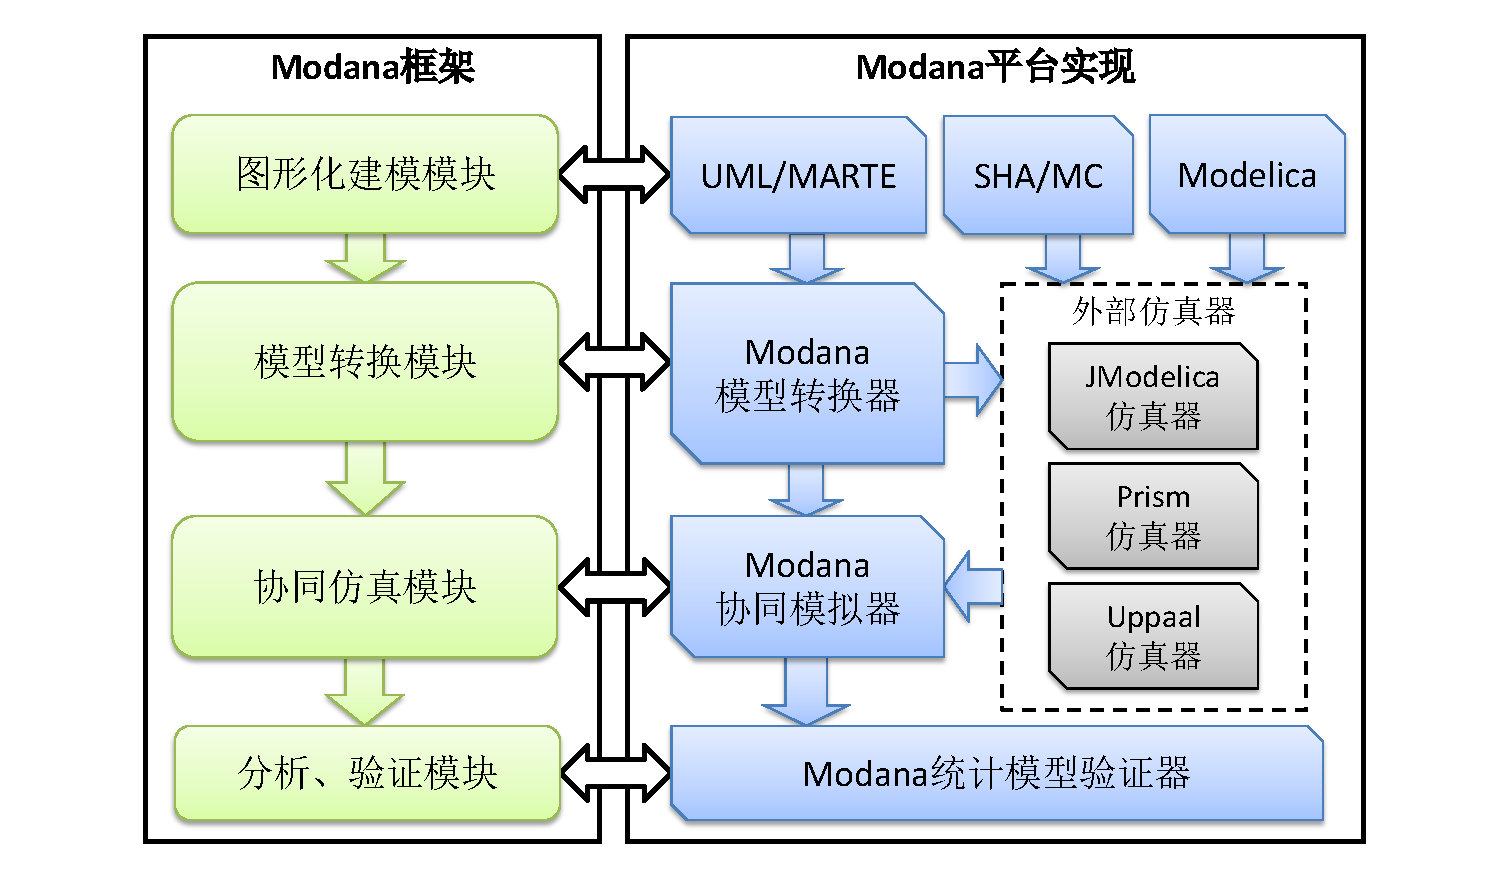
\includegraphics[width=4in]{modana.pdf}
	\caption{Modana体系结构}
	\label{modana}
	\end{figure}
	
	%基于Modana平台,可以实现本文提出的扩展的MARTE/UML状态图的建模以及模型转换为ESHA。
	%UPPAAL-SMC\citep{DBLP:journals/spe/BehrmannDLPY11,DBLP:journals/corr/abs-1207-1272}是时下最流行的模型检测工具之一,它提供了图形化建模SHA的功能,并利用统计模型检测方法(Stochastic Model Checking,SMC)实现对模型的定性、定量分析,且验证效率较高。

	基于3.3.3节中扩展的MARTE/UML状态图定义和4.1.1节中的ESHA定义,以及模型映射规则,在Modana平台的基础上,我们实现了扩展MARTE/UML状态图到ESHA的自动转换。利用Modana前端建模模块,可以实现扩展的MARTE/UML状态图的建模,并导出XML格式的模型文件。而UPPAAL-SMC的能耗随机混成自动机模型文件格式也为XML形式,模型转换实质上为两种XML文件对应节点的转换,这为实现扩展的MARTE/UML状态图到ESHA的转换提供了技术基础。
	
	\begin{figure}[!t]
	\centering
	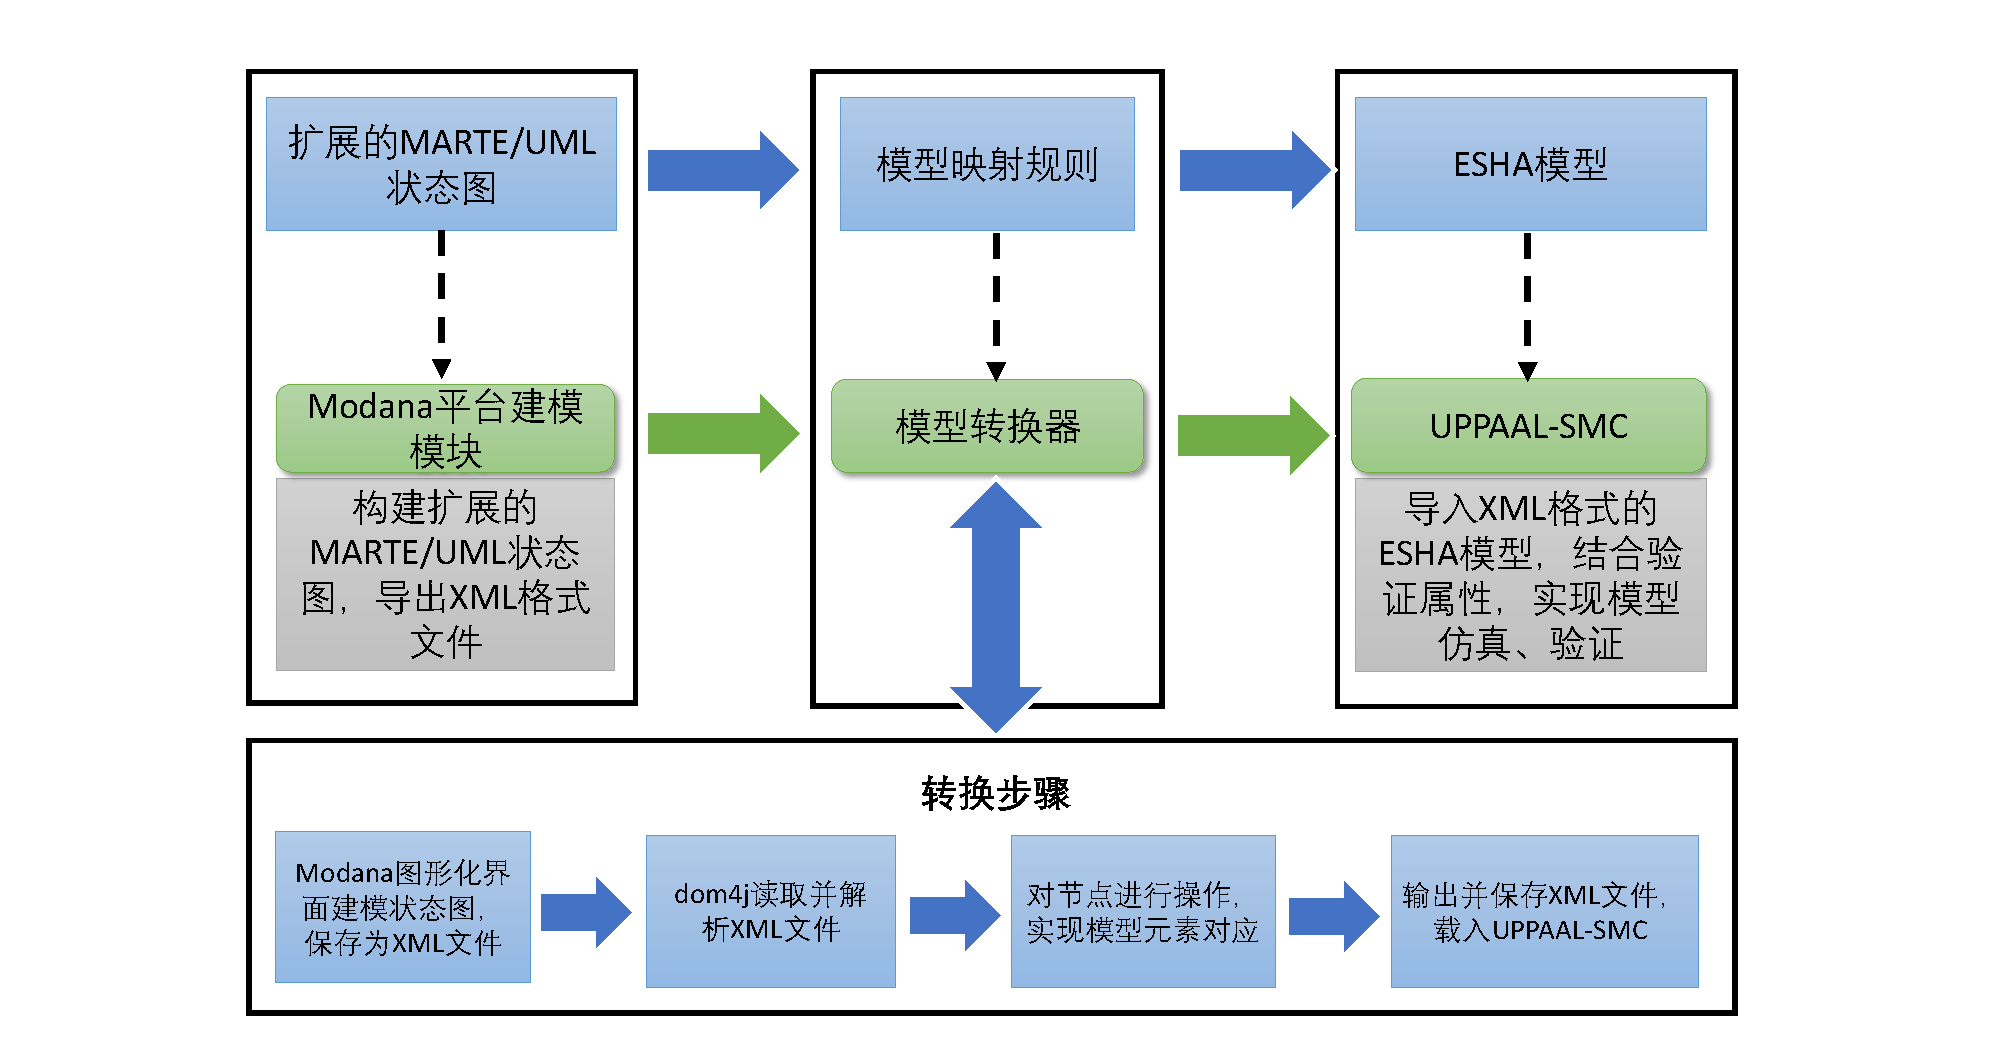
\includegraphics[width=4.6in]{tran.pdf}
	\caption{基于Modana和UPPAAL-SMC的实现框架}
	\label{tools}
	\end{figure}
	
	如图\ref{tools}所示,基于Modana和UPPAAL-SMC工具,可以实现本文提出的智能建筑能耗的建模与分析方法。
	
	在模型转换过程中,我们使用了dom4j来操作模型文件。dom4j是Java的一个XML API,可以用来读写XML文件。它可以实现建立XML文档,添加、修改、删除节点,以及格式化输出等功能。dom4j具有性能优异、功能强大且简单易用的优点,同时它也是一个开源库。本文基于Modana前端建模模块,使用dom4j读取扩展的MARTE/UML状态图XML文件,查询文件中的元素,通过序列化XML文档生成对应的ESHA模型文件,最后,载入UPPAAL-SMC中实现模型验证。具体步骤如下:
	\begin{itemize}
	\item 通过Modana前端建模模块绘制扩展的MARTE/UML状态图,并存储为XML文件;
	\item 使用dom4j读取扩展的MARTE/UML状态图的XML文件,查询XML节点,筛选出模型元素;
	\item 通过模型映射规则,修改XML节点,实现对应元素映射;
	\item 导出序列化XML文件,载入UPPAAL-SMC中,输入验证属性实现模型仿真、验证。
	\end{itemize}
	
	
	%\begin{itemize}
	%\item 状态映射:初始状态对应于初始位置;终止状态对应于终止位置;Invariant衍型的状态,其constraint的不变式表达式对应于ESHA位置上的不变式约束;CEvolution衍型的状态,其cevolution的微分表达式对应于ESHA位置上的微分等式;CEConsump衍型的状态,其ceconsump的能耗微分表达式对应于ESHA位置上的能耗微分等式;TimeDelay衍型的状态,其timedelay的时延概率分布对应于ESHA位置上的时钟迁移约束;
	%\item 迁移映射:状态图中迁移的源状态和目标状态分别对应于ESHA中的源位置和目标位置,警备条件、触发事件、执行效应以及迁移概率也都一一对应;在状态图中,一个EventEconsump衍型的迁移,其触发事件所消耗的能量在ESHA中被定义为执行效应中对eventeconsump变量的重新赋值;一个ActionEconsump衍型的迁移,其执行效应所消耗的能量在ESHA中被定义为执行效应中对actioneconsump变量的重新赋值。
	%\end{itemize}
	
\section{本章小结}
	尽管MARTE/UML模型可以实现系统的多视图建模,但由于其半形式化的特点,无法实现系统的仿真、验证。因此,为了对系统模型进行进一步分析,本章在随机混成自动机的基础上,提出了能耗随机混成自动机的概念,支持系统能耗的显式建模,且可以利用统计模型检测方法对其进行系统属性的高效验证。为了将MARTE/UML模型和ESHA联系起来,我们给出了扩展的状态图到ESHA的映射规则和算法,并基于我们的Modana工具和模型验证工具UPPAAL-SMC,给出了本文所提的智能建筑能耗建模与分析方法的实现框架。




\chapter{案例研究}
\label{ch5}
	温控系统是智能建筑的重要组成部分之一,在本章,我们以一个智能办公建筑为例,研究该智能建筑中温控系统的作用,以验证本文所提方法的可行性和实用性。案例改编自Ansgar等学者在\citep{DBLP:conf/hybrid/FehnkerI04} 中提出的Room Heating Benchmark,与之前的研究\citep{DBLP:journals/chinaf/DavidDLMS12,不确定环境下智能大厦空调系统调度策略评估,DBLP:conf/compsac/ChenGCDLS15}相比,本案例考虑了更多实际因素:物理环境温度变化的实际模型、办公场景下用户行为的各种模式、人的散热对室内温度的影响以及实时电价的差异。此外,在\citep{DBLP:journals/chinaf/DavidDLMS12,不确定环境下智能大厦空调系统调度策略评估,DBLP:conf/compsac/ChenGCDLS15}中,研究人员根据自己的专业知识,直接给出了系统的可验证模型。而本案例展示了利用领域本体指导构建系统初步模型、模型精化、借助模型转换技术得到系统的ESHA,实现有关系统能耗等性质的验证与分析的完整过程。
	
\section{场景描述}
	一个智能办公建筑中包含一定数目的办公室、会议室和加热器。加热器的数量比房间少,且每个房间最多只能使用一个加热器。由于墙的热传导性,不断变化的外界环境温度以及相邻房间温度会对某个房间的室内温度造成影响。同时,办公建筑中的用户行为也会间接影响室内温度。加热器由一个简单恒温器控制,当房间温度低于某个特定阈值时,加热器打开;当房间温度高于某个特定阈值时,加热器关闭。在智能温控系统中,能耗主要来源于加热器的工作以及系统中的信号传输。
	%由于墙的热传导性,不同房间之间以及房间与外界环境之间存在热传递。对于房间i,与其他房间的热交换系数记作$a_{i,j}$,	与物理环境的热交换系数记作$b_{i}$,加热器对其作用的功率记作$c_{i}$。
	
\section{系统建模}
\subsection{初步模型}	
	依照第三章给出的智能建筑领域本体,我们首先对系统进行需求分析,并指导建模系统的扩展MARTE/UML初步模型。	
	\begin{figure}[!t]
	\centering
	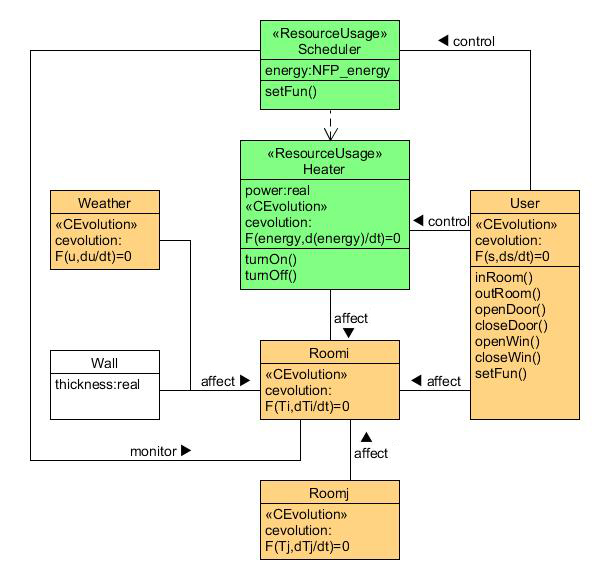
\includegraphics[width=3.8in]{sb-cd.jpg}
	\caption{智能办公建筑的类图}
	\label{sb-cd}
	\end{figure}
	
	\begin{figure}[!t]
	\centering
	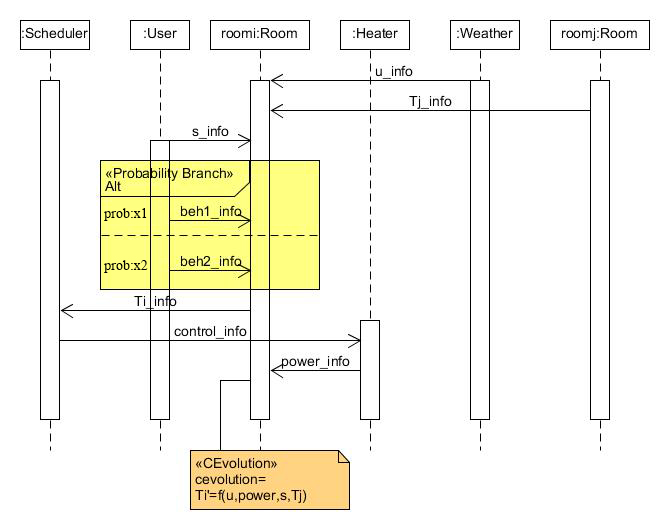
\includegraphics[width=4.2in]{sb-sd.jpg}
	\caption{智能办公建筑的顺序图}
	\label{sb-sd}
	\end{figure}
	
	\begin{figure}[!t]
	\centering
	\subfigure[物理环境]{
	\begin{minipage}[b]{0.3\textwidth}
	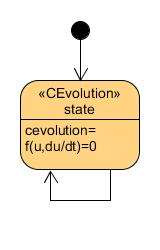
\includegraphics[width=0.6\textwidth]{weather-sm1.jpg} 
	\end{minipage}
	\label{weather-sm1}
	}
	\subfigure[加热器]{
	\begin{minipage}[b]{0.4\textwidth}
	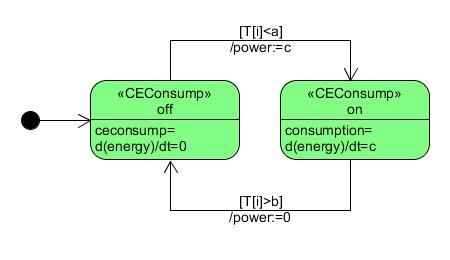
\includegraphics[width=1.2\textwidth]{heater-sm1.jpg} 
	\end{minipage}
	\label{heater-sm1}
	}
	\subfigure[室内环境]{
	\begin{minipage}[b]{0.3\textwidth}
	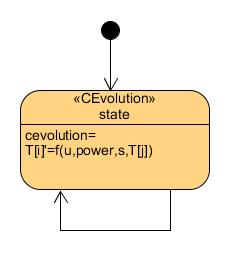
\includegraphics[width=0.8\textwidth]{room-sm1.jpg} 
	\end{minipage}
	\label{room-sm1}
	}
	\caption{物理环境、加热器和室内环境的初步状态图}
	\label{sm1}
	\end{figure}
	
	\begin{itemize}
	\item 首先,易知,在本案例中,我们研究的建筑环境参数是室内温度;
	\item 结合2.1.3节中定义的室内环境参数约束的第二条,可以找到相关的概念有:物理环境温度、相邻房间温度、墙的热传导性能、用户的离开/进入房间行为、开/关门行为、开/关窗行为、人的散热、加热器的作用以及调度器对加热器的控制;
	\item 根据概念间的相关关系,可以确定,涉及到的系统实体概念有:物理环境、加热器、房间室内环境、墙、用户和调度器,利用扩展的MARTE类图的定义,为它们分别创建如图\ref{sb-cd}所示的类图,前述的参数概念和行为概念对应各自类的属性和操作。易知,在智能温控系统中,耗能类是加热器和调度器,在之后的状态图建模中,我们将密切关注能量在对象内部的产生与消耗情况;
	\item 根据概念的上下文图(图\ref{context}),可知:物理环境和相邻房间的实时温度参数会影响室内环境;用户的散热和随机行为也会影响室内环境;加热器受调度器的控制,且其作用会对室内环境造成影响。而墙这种物理构成的参数是一个固定值,无需对其创建对象。基于上下文图,可建模如图\ref{sb-sd}所示的扩展MARTE/UML顺序图。首先,物理环境和相邻房间的温度信息会传递给当前房间$room_{i}$;用户自身的散热会影响室内温度,同时,用户有一定的概率执行随机行为$beh1$,一定的概率执行随机行为$beh2$,且其行为也会对室内温度造成影响;调度器以一定频率监测$room_{i}$的温度,并按照某种调度策略来控制加热器;加热器的加热功率直接影响室内温度;在$room_{i}$的控制焦点上,我们添加了$CEvolution$衍型来定义室内环境与其他因素的函数关系;
	\item 依照2.2节中给出的不同实体概念的模板构建状态图:对于物理环境,由于系统无法对其产生控制和影响,即它的状态不会被改变,因此,在状态图中,可以用表达式来描述物理环境参数的变化;对于加热器,在不考虑异常情况时,它通常应该在开启和关闭两个状态间切换,关闭时不耗能,开启时以一定速率耗能,且开启时其对室内环境的作用为其功率参数;对于用户,其行为是随机的,且每一个行为的发生会改变其状态;对于调度器,在一定的判断准则下,对加热器进行控制,且控制信号的传输会带来能耗;对于室内环境,它的温度参数受到以上几个实体的作用而变化。通过以上分析,可以得到物理环境、加热器和室内环境的初步状态图,如图\ref{sm1}所示。以上模型的状态变化符合一定的规则,可以抽象为固定模板,而用户行为具有较强的随机性,系统调度器的判断逻辑较为复杂,在下一节,我们将通过深入分析,给出办公场景下几种常见的用户行为模式和调度器的几种不同策略。
	\end{itemize}

\subsection{精化模型}
	在智能温控系统中,物理环境温度、室内温度和系统能耗的连续变化体现了系统的混成特性;而系统的随机性主要体现在用户行为的不确定;系统能耗的产生主要来源于两方面——加热器的工作、调度器和加热器之间的信号传输,其他对象通过影响调度器对加热器的决策间接影响能耗。	
	
	%在预设的场景中,由于加热器的数量少于房间数量,当出现多个房间需要加热器时,房间之间会产生竞争关系。此时,调度器必须按一定的规则对加热器进行调度。因此,对温控系统建模的一个重点是调度器的设计。通过领域本体可以指导我们建模智能建筑中的物理环境、室内环境和功能构件这些行为模式比较固定的实体概念的状态图。而对于系统调度器和用户这些实体,其内部状态变化较为复杂,下面,我们通过深入分析来进一步精化系统模型。
		
	在智能建筑领域本体中,我们已经定义了:室内温度与外界温度(物理环境温度和相邻空间温度)、墙的热传导性能、用户的离开/进入房间、开/关门行为、开/关窗行为、人的热量、暖通空调的作用以及调度器的控制有关。在本案例中,为了简化模型,对于用户行为仅考虑其离开/进入房间的影响。参考文献\citep{DBLP:conf/hybrid/FehnkerI04},本案例中房间i的室内环境温度可以由以下公式定义:
	
	\begin{equation}
	T_{i}^{'} = \sum_{j\not=i} a_{i,j}(T_{j}-T_{i})+b_{i}(u-T_{i})+c_{i}h_{i}+s(T_{i})N_{i}
	\label{gongshi}
	\end{equation}
	
	其中,变量$T_{i}$和$T_{j}$分别表示房间i和房间j的室内温度,变量$u$代表物理环境温度。$h_{i}$是一个布尔类型的变量,其值为1时代表加热器被房间i使用,其值为0时代表房间i并未使用加热器。常量$a_{i,j}$称作房间i和房间j的热交换系数,由墙的热传导性能和房间之间的相互位置决定。热传导系数具有对称性,即$a_{i,j}=a_{j,i}$,若房间i和房间j不相邻,则$a_{i,j}=0$。常量$b_{i}$和$c_{i}$分别表示房间i与物理环境的热传递系数和加热器对房间i的加热功率。$s(T_{i})$是指在室内温度为$T_{i}$的情况下人体产生的热量,$N_{i}$代表房间i内的人数。之前关于智能建筑温控系统的研究中均没有考虑到人的散热,实际上,在人数较多的办公环境中,对于室内温度而言,人的散热会带来不可忽略的影响。

	按照一个成年人的平均体重为68公斤的标准,结合\citep{CarrierCorporation1965Handbook}中人在不同温度下散热的数据,我们使用MATLAB工具进行仿真拟合,得到了人体散热与房间温度的关系为:
	\begin{equation}
	s(T)=98.62e^{-(\frac{T-14.03}{17.41})^2}
	\end{equation}
	%Each heater is equipped with a bang-bang controller congured to turn the heating on (hi := 1) when temperature Ti falls below the predened threshold oni and turn it back o (hi := 0) when temperature Ti becomes greater than oi . The central controller can switch over the heating from one room to another.290 Provided that there are two or more rooms that need to be heated at the same time, the controller may reallocate heaters according to predened strategies. By this way, heaters are shared by dierent rooms to meet some requirements on occupant comfortability or energy consumption. The room needs a heater if the temperature drops below its get threshold. The occupants feel uncomfortable when the room temperature drops below low. The controller adopts various control strategies to maintain the room temperature for 295 comfortable occupant feeling or optimize energy consumption. The denition and default setting of oni ,oi , get and low can be found in
	
	每个加热器由一个``bang-bang controller''控制:当房间i的温度$T_{i}$低于预设的开启温度$on_{i}$时,加热器开启,并将变量$h_{i}$置为1;当房间i的温度$T_{i}$高于预设的关闭温度$off_{i}$时,加热器关闭,并将变量$h_{i}$置为0。调度器可以将加热器从一个房间切换到另一个房间。当有超过两个房间同时需要加热时,调度器将使用某种策略来对加热器进行配置。通过这种方式,加热器得以被不同的房间共享使用,来保证室内用户的舒适度。当房间i的温度低于$get_{i}$($get_{i}<on_{i}$)时,代表它需要加热器。用户在房间的温度低于$low_{i}$($low_{i}<get_{i}$)时,会感到不舒服。调度器的智能控制需要保持室内温度在用户舒适度的范围内且尽量优化能耗。关于$on_{i}$、$off_{i}$、$get_{i}$和$low_{i}$的详细定义可以参考文献\citep{DBLP:conf/compsac/ChenGCDLS15}。
	
	在本案例中,我们考虑三种参数维度:
	\begin{enumerate}
	\item 物理环境温度:我们设计了四种不同的温度模拟方式,包括恒温、简单正弦函数模拟、复杂正弦函数模拟和高斯函数模拟;
	\item 调度策略:我们使用了三种调度策略,主要差异在于加热器使用权移动的判断方式不同;
	\item 用户行为模式:考虑到实际智能建筑中常见的办公情形,我们设计了三种用户行为模式,分别为日常工作模式、工作/出差模式和会议模式。在不同的用户行为模式中,用户行为通过改变上述的预设值——$on_{i}$、$off_{i}$、$get_{i}$和$low_{i}$和公式\ref{gongshi}中的系数,来影响调度器的调度,从而影响系统能耗。
	\end{enumerate}

\textbf{1、精化后的物理环境模型}

	\begin{figure}[!t]
	\centering
	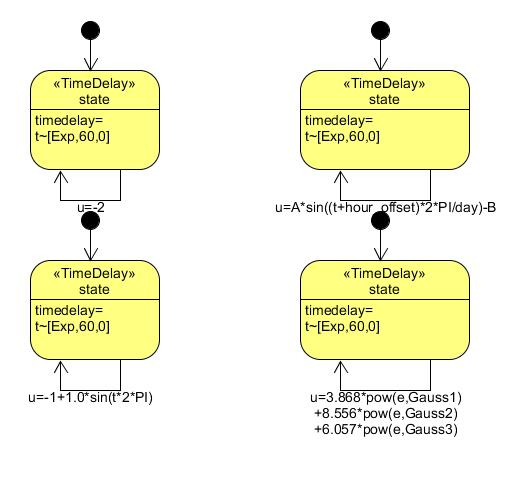
\includegraphics[width=3.2in]{weather-sm2.jpg}
	\caption{精化后的物理环境状态图}
	\label{weather-sm2}
	\end{figure}
	
	对于物理环境,不同于初步模型中直接将温度模拟公式附在状态上的方式。考虑到现实情况中,智能建筑的传感器按照一定频率对物理环境温度进行监测,我们将模型进行调整:将温度模拟公式添加到迁移上,并为状态设置一个指数型的时延概率分布,表示系统以每个时间单位60次的频率监测物理环境温度。
	
	如图\ref{weather-sm2}所示:图a表示物理环境恒定温度为-2摄氏度;图b表示一个简单的正弦函数模拟的温度;图c中的参数A和B为自定义值,可以更准确地模拟温度的实际情况;图d中的温度由高斯函数模拟,是我们根据上海2-3月份的实际温度情况在MATLAB工具中模拟后计算所得,最终的高斯曲线拟合结果为$u = 3.868e^{gauss1(t)} + 8.556e^{gauss2(t)} + 6.057e^{gauss3(t)}$,其中$gauss1(t) = -(\frac{t-23.16}{11.58})^2$,$gauss2(t) = - (\frac{t-14.24}{6.194})^2$,$gauss3(t) = -(\frac{t+1.212}{5.069})^2$。

\textbf{2、精化后的加热器模型}

	\begin{figure}[!t]
	\centering
	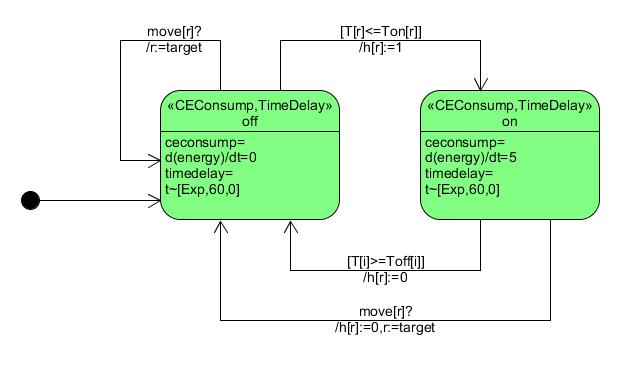
\includegraphics[width=3.8in]{heater-sm2.jpg}
	\caption{精化后的加热器状态图}
	\label{heater-sm2}
	\end{figure}
	
	在考虑了调度器的调度策略后,加热器在开启和关闭状态时必须接收来自调度器的信号,以确认是否转移作用的房间。当加热器关闭时,接收到调度器发送的$move[r]?$信号时,将变量$target$的值赋给$r$,即锁定将要判断的为房间r的温度;当加热器开启时,需要先将加热器使用权从当前的房间r夺走,再将$target$的值赋给$r$。此外,设置布尔型标记$h[i]$来表示房间i是否占有加热器,$h[i] \times c[i]$表示加热器对房间i的作用,则无需在开关状态切换时对加热功率$power$进行重新赋值。精化后的加热器状态图如图\ref{heater-sm2}所示。
	
\textbf{3、精化后的室内环境模型}

	\begin{figure}[!t]
	\centering
	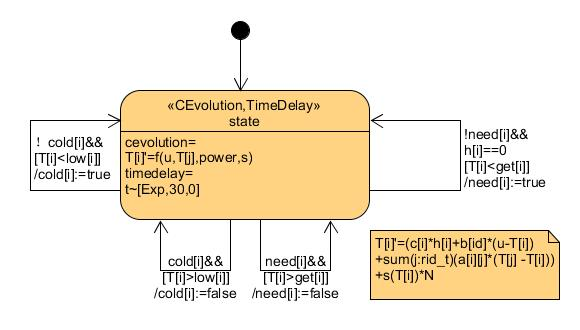
\includegraphics[width=3.6in]{room-sm2.jpg}
	\caption{精化后的室内环境状态图}
	\label{room-sm2}
	\end{figure}
	
	对于室内环境来说,结合前述关于$on_{i}$、$off_{i}$、$get_{i}$和$low_{i}$的介绍,我们将对室内温度的判断加在室内环境状态图中,并通过设置一些标记值来供调度器判断。如图\ref{room-sm2}所示,当房间i室内温度$T[i]$低于预设值$low[i]$时,代表室内温度已经不满足人的舒适度要求,将标记变量$cold[i]$置为$true$,反之为$false$;当$T[i]$高于预设值$get[i]$时,代表在当前的室内温度下,已经不需要加热器了,将标记变量$need[i]$置为$false$,反之为$true$。
	
\textbf{4、用户行为模型}
	\begin{figure}[!t]
	\centering
	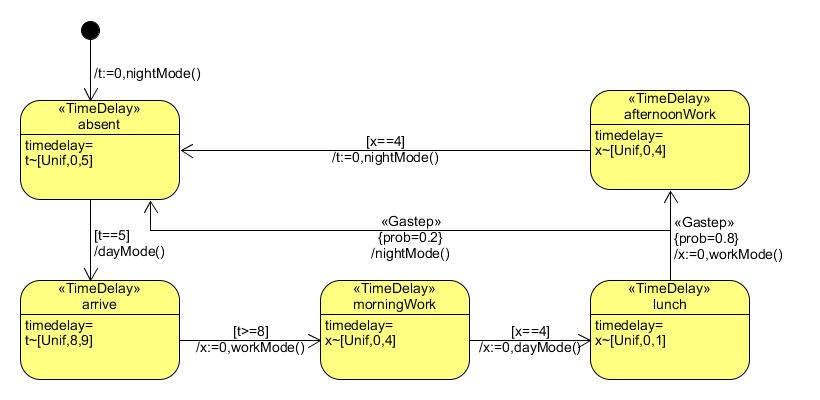
\includegraphics[width=4.8in]{user-sm.jpg}
	\caption{工作/出差模式状态图}
	\label{user-sm}
	\end{figure}
	
	在领域本体中,我们介绍了用户可以执行的行为,如离开/进入房间、开/关门、开/关窗等。之前的研究仅考虑了用户进入/离开房间这样的简单动作行为,本案例更贴合实际,考虑了办公场景中,职工的上班、下班、出差和开会这些常见的行为,并设计了三种用户行为模式:1)日常工作模式:用户早晨来到办公室上班、进行上午的工作、离开办公室去吃午饭、进行下午的工作,最后下班离开办公室;2)工作/出差模式:除了正常工作外,职工在下午可能会出差拜访客户等,由此可以设置工作/出差模式;3)会议模式:在某个项目刚开始的时期,为了确定项目方案,职工可能早上、下午均需要去会议室参加会议商讨方案。
	
	图\ref{user-sm}展示了工作/出差模式的状态图。最初,在凌晨至上午5点,办公建筑处于夜间模式,此时的$on_{i}$、$off_{i}$、$get_{i}$数值均处于预设的较低值;上午5点之后,办公建筑进入预热状态,即被$on_{i}$、$off_{i}$、$get_{i}$被设定为更高的值,开启白天模式;职工可能在上午8点至9点间的任意时刻来到办公建筑,当职工到达后,办公建筑被配置为工作模式,即对于室内环境来说,需要考虑办公室中人群的散热情况;之后,职工开始上午的工作,工作4小时后,他们会出去吃午饭,此时办公建筑再次被配置为白天模式,即不考虑人的散热情况;午饭时间为[0,1]时内的均匀分布,午饭回来后,职工有$80\%$的可能性继续下午的工作,$20\%$的可能性出去见客户,即直接离开办公建筑;若职工继续下午的工作,将连续工作4小时后下班,并离开办公建筑。
	
\textbf{5、调度器模型}	

	对于何时将房间j占有的加热器分配给房间i,即房间之间的竞争条件,我们考虑以下三种调度策略:	
	\begin{enumerate}
	\item 策略$\uppercase\expandafter{\romannumeral1}$:房间i的温度小于$get_{i}$,即$T_{i} < get_{i}$,且房间j和房间i的温差大于一定值,即$T_{j}-T_{i} \geq dif_{i}$;
	\item 策略$\uppercase\expandafter{\romannumeral2}$:房间i的温度小于$get_{i}$,即$T_{i} < get_{i}$,且房间j的温度大于$on_{j}$,即$T_{j} \geq on_{j}$;
	\item 策略$\uppercase\expandafter{\romannumeral3}$:房间i的温度小于$get_{i}$,即$T_{i} < get_{i}$,且房间j的温度大于$get_{j}$($get_{j}<on_{j}$),即$T_{j} \geq get_{j}$;
	\end{enumerate}

	下面,以策略$\uppercase\expandafter{\romannumeral1}$为例,我们将分析并给出调度器的扩展MARTE/UML状态图。
	
	\begin{figure}[!t]
	\centering
	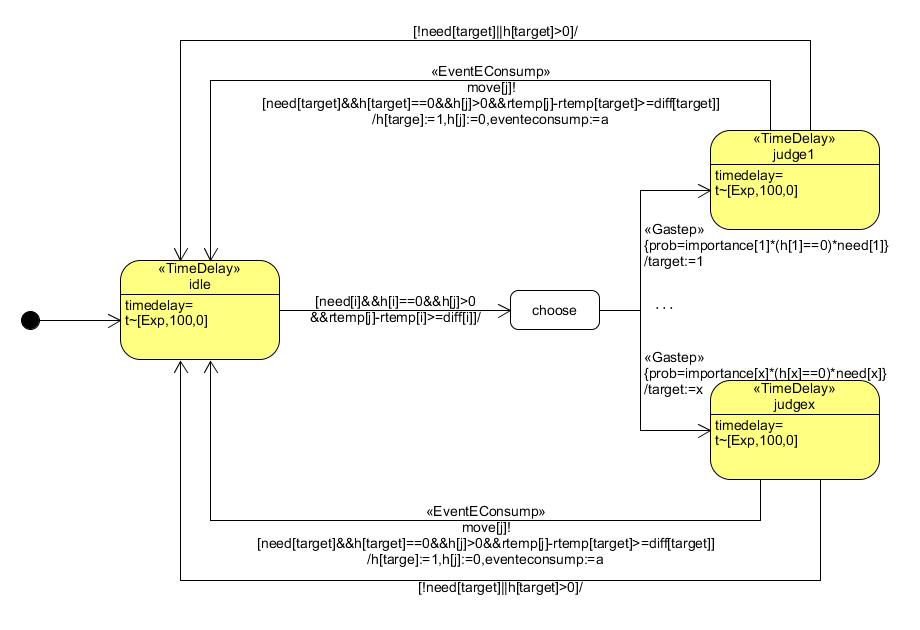
\includegraphics[width=4.9in]{scheduler-sm.jpg}
	\caption{策略$\uppercase\expandafter{\romannumeral1}$的状态图}
	\label{scheduler-sm}
	\end{figure}
	
	如图\ref{scheduler-sm}所示,当调度器处于空闲状态时,其以每单位时间(小时)100次的频率来监测室内环境的状态,这一随机行为由指数时延概率分布描述;当调度器监测到有房间需要加热且不占用加热器,同时存在另一个房间与其温差大于预设值$dif$时,调度器将发生状态迁移,进入选择状态;随后,调度器将对所有需要加热且不占用加热器的房间按照其重要性系数$imp$进行离散的概率选择;若调度器选择了房间x,则进入判断状态并将x设为加热器将要移动的目标$target$;随后,调度器判断此时是否仍存在一个占有加热器的房间,且其与房间x的温差大于$dif$,若成立,则将该房间的加热器赋予房间x,否则不执行任何操作。值得注意的是,在判断需要将某房间的加热器赋予房间x时,调度器会向该加热器发送信号,此时的信号传输需要消耗一定能量。
	
\section{模型验证与分析}
	在前面的系统建模步骤中,我们已经得到了系统的设计模型,但若要对系统进行验证,除了利用前述的转换算法将扩展的MARTE/UML状态图转换为ESHA模型外,还需要进行参数实例化,以验证特定参数组合下系统的性质,并分析系统的能耗。
	
	我们考虑一个具体的应用场景,某智能办公建筑的平面图如图\ref{building}所示,共包含一个会议室、五个办公室和三个加热器,且初始状态加热器1、加热器2、加热器3分别供房间2、房间4和房间6使用。
	
	\begin{figure}[!t]
	\centering
	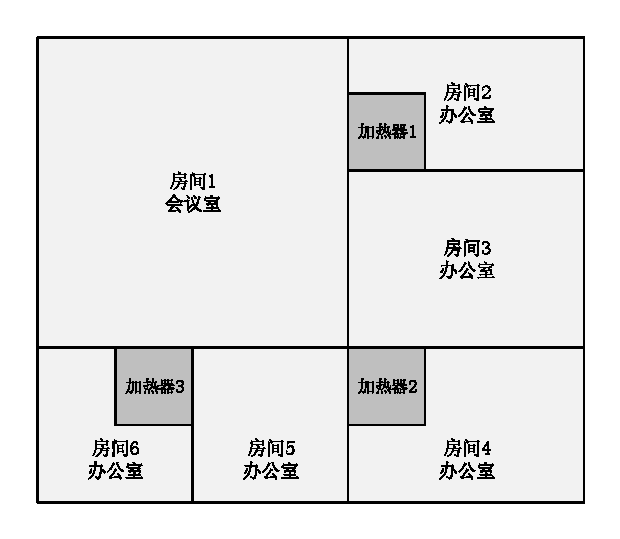
\includegraphics[width=3in]{building.pdf}
	\caption{智能办公建筑的布局}
	\label{building}
	\end{figure}
	
	在本案例中,参考文献\citep{DBLP:journals/chinaf/DavidDLMS12}中的数据,房间热交换系数、不同房间与物理环境的热交换系数和加热器对不同房间的加热功率设置如图\ref{room-para}。
	\begin{figure}
	\centering
	\subfigure[房间热交换系数]{
	\begin{minipage}[b]{0.3\textwidth}
	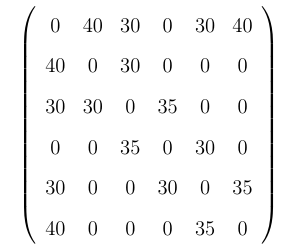
\includegraphics[width=1\textwidth]{aij.png} 
	\end{minipage}
	\label{aij}
	}
	\subfigure[物理环境热交换系数]{
	\begin{minipage}[b]{0.32\textwidth}
	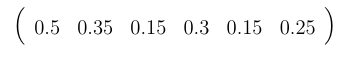
\includegraphics[width=1.1\textwidth]{bi.png} 
	\end{minipage}
	\label{bi}
	}
	\subfigure[加热器功率]{
	\begin{minipage}[b]{0.25\textwidth}
	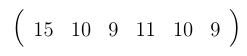
\includegraphics[width=1\textwidth]{ci.png} 
	\end{minipage}
	\label{ci}
	}
	\caption{案例参数实例化}
	\label{room-para}
	\end{figure}
%\begin{figure}
%\centering
%\subfigure[房间的热交换系数]{
%\begin{minipage}[b]{0.3\textwidth}
%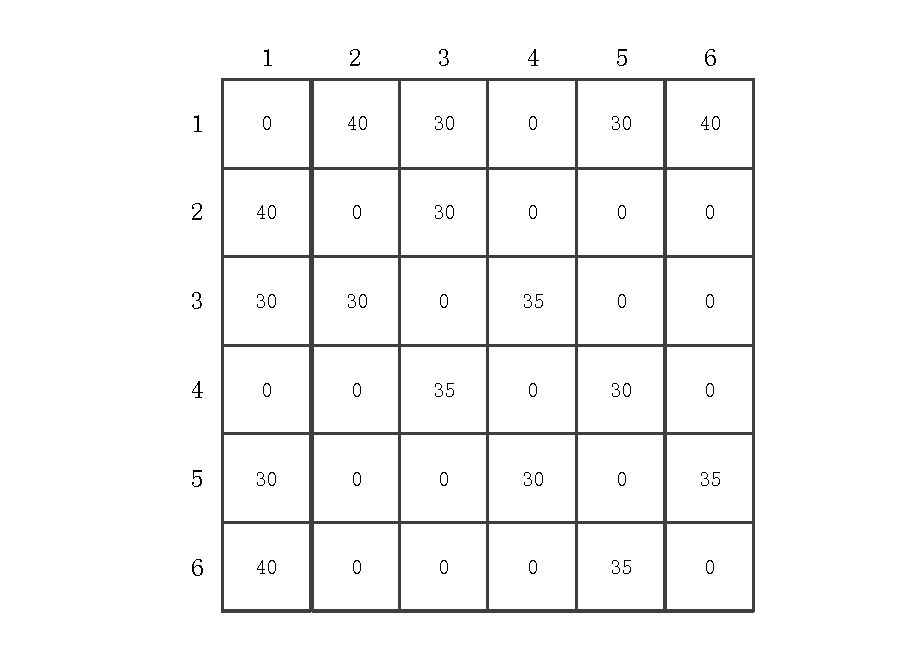
\includegraphics[width=1.5\textwidth]{room-a.pdf} 
%\end{minipage}
%\label{room-a}
%}

%\begin{equation}       
%\left(                 
%  \begin{array}{cccccc}   
%    0  & 40 & 30 & 0  & 30 & 40\\
%    40 & 0  & 30 & 0  & 0  & 0 \\
%    30 & 30 & 0  & 35 & 0  & 0 \\
%    0  & 0  & 35 & 0  & 30 & 0 \\
%    30 & 0  & 0  & 30 & 0  & 35\\
%    40 & 0  & 0  & 0  & 35 & 0 \\   
% \end{array}
%\right)                 
%\end{equation}

%\subfigure[不同房间与外界温度的热交换系数]{
%\begin{minipage}[b]{0.3\textwidth}
%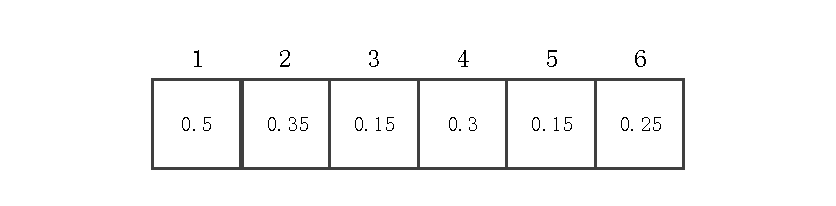
\includegraphics[width=1.5\textwidth]{room-b.pdf} 
%\end{minipage}
%\label{room-b}
%}
%\begin{equation}       
%\left(                 
%  \begin{array}{cccccc}   
%    0.5  & 0.35 & 0.15 & 0.3  & 0.15 & 0.25
%  \end{array}
%\right) 
%\end{equation}
%\subfigure[加热器对不同房间的功率]{
%\begin{minipage}[b]{0.3\textwidth}
%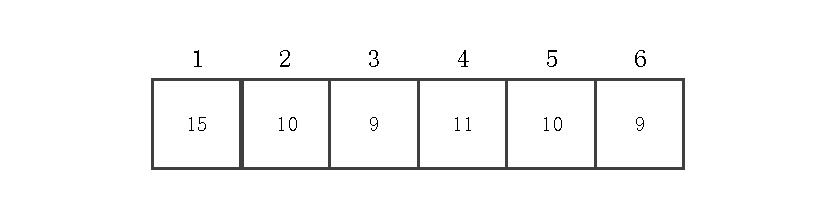
\includegraphics[width=1.5\textwidth]{room-c.pdf} 
%\end{minipage}
%\label{room-c}
%}
%\caption{案例参数实例化}
%\label{room-para}
%\end{figure}

%\begin{equation}     
%\left(                 
%  \begin{array}{c c c c c c c}   
%    15  & 10 & 9 & 11  & 10 & 9   
%  \end{array}
%\right)                 
%\end{equation}
\subsection{ESHA模型}
	对于本案例,完整的ESHA网络模型包括:物理环境模型、加热器模型、室内环境模型、用户行为模式模型、调度器模型和实时电价模型六部分。

	利用Modana模型转换器,我们将前述的MARTE/UML模型转换为UPPAAL工具可识别的ESHA模型,并使用UPPAAL工具载入该模型文件以图形化显示,为了模型的美观性,我们手动对模型进行了适当的修改(主要是将一些计算公式进行了函数封装)。
	
	图\ref{weather-esha}为四种物理环境模式的ESHA模型。其中,weatherGauss模型在$update()$函数中定义了如何利用高斯函数来模拟温度的具体公式。
	
	\begin{figure}
	\centering
	\subfigure[weatherFlat]{
	\begin{minipage}[b]{0.4\textwidth}
	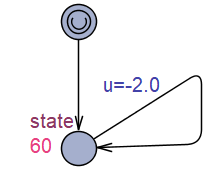
\includegraphics[width=0.45\textwidth]{weather-esha1.png} 
	\end{minipage}
	\label{weather1}
	}
	\subfigure[weatherSimple]{
	\begin{minipage}[b]{0.4\textwidth}
	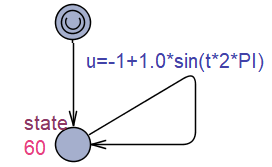
\includegraphics[width=0.6\textwidth]{weather-esha2.png} 
	\end{minipage}
	\label{weather2}
	}
	\subfigure[weatherComplex]{
	\begin{minipage}[b]{0.4\textwidth}
	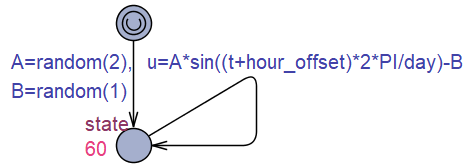
\includegraphics[width=1.0\textwidth]{weather-esha3.png} 
	\end{minipage}
	\label{weather3}
	}
	\subfigure[weatherGauss]{
	\begin{minipage}[b]{0.4\textwidth}
	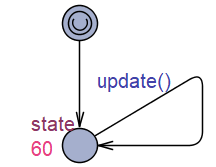
\includegraphics[width=0.45\textwidth]{weather-esha4.png} 
	\end{minipage}
	\label{weather4}
	}
	\caption{四种物理环境模式的ESHA模型}
	\label{weather-esha}
	\end{figure}
	
	图\ref{heater-esha}为加热器和室内环境的ESHA模型。
	
	\begin{figure}
	\centering
	\subfigure[heater]{
	\begin{minipage}[b]{0.4\textwidth}
	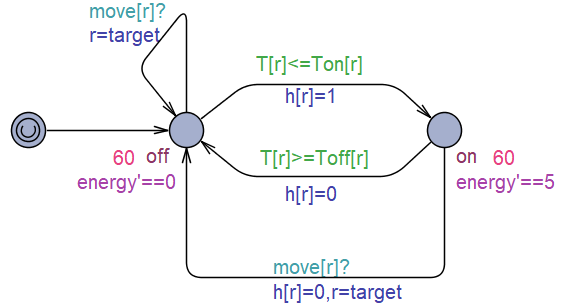
\includegraphics[width=1.05\textwidth]{heater-esha.png} 
	\end{minipage}
	\label{heater-esha}
	}
	\subfigure[room]{
	\begin{minipage}[b]{0.4\textwidth}
	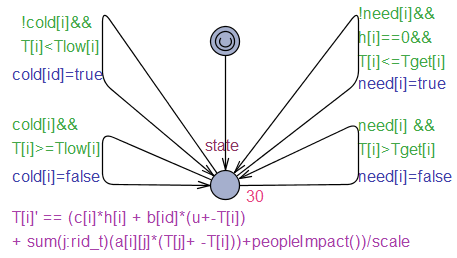
\includegraphics[width=1.05\textwidth]{room-esha.png} 
	\end{minipage}
	\label{room-esha}
	}
	\caption{加热器和室内环境的ESHA模型}
	\label{heater-esha}
	\end{figure}

	如前文所述,用户模式分为日常工作模式、工作/出差模式和会议模式,三种用户模式的ESHA模型如图\ref{user-esha}所示。
	
	\begin{figure}
	\centering
	\subfigure[work]{
	\begin{minipage}[b]{0.4\textwidth}
	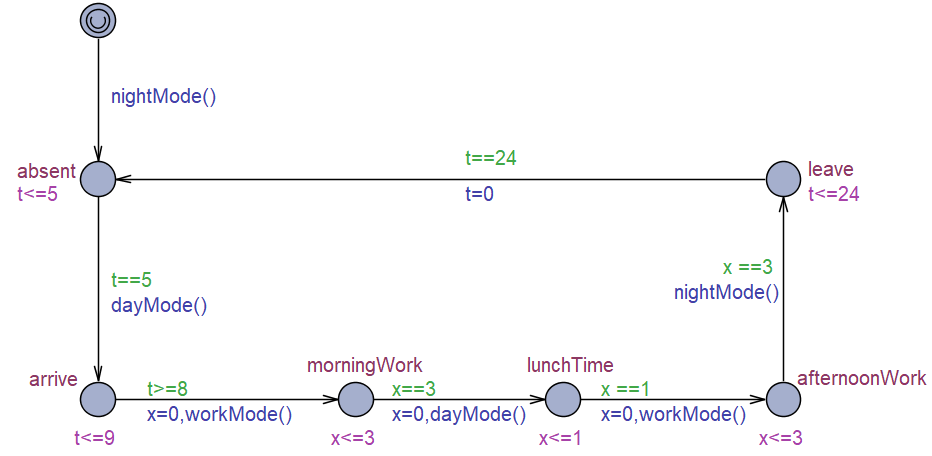
\includegraphics[width=1.05\textwidth]{user-esha1.png} 
	\end{minipage}
	\label{user-work}
	}
	\subfigure[work/out]{
	\begin{minipage}[b]{0.4\textwidth}
	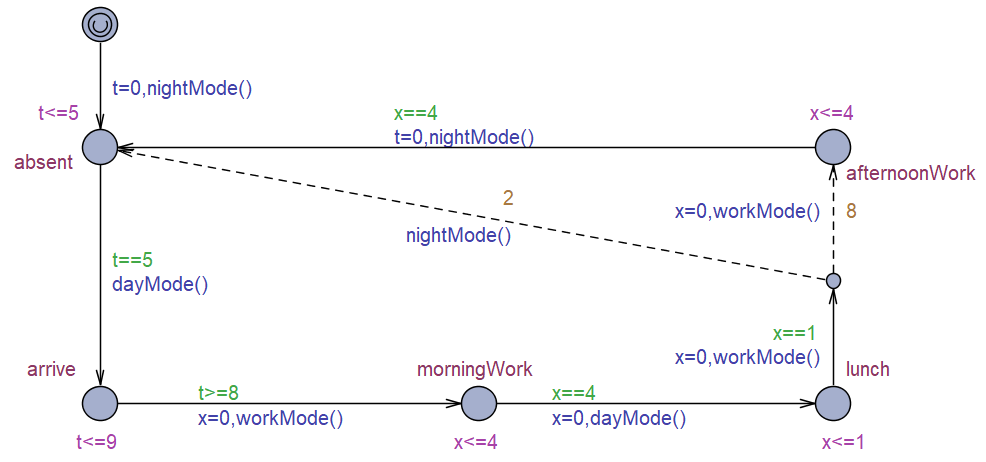
\includegraphics[width=1.05\textwidth]{user-esha2.png} 
	\end{minipage}
	\label{user-prob}
	}
	\subfigure[conference]{
	\begin{minipage}[b]{0.4\textwidth}
	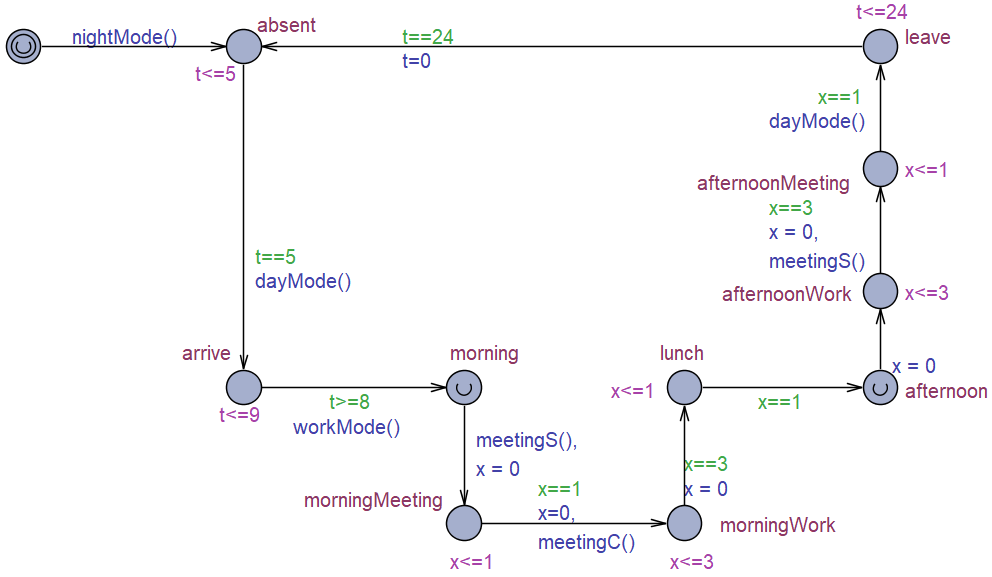
\includegraphics[width=1.05\textwidth]{user-esha3.png} 
	\end{minipage}
	\label{user-conference}
	}
	\caption{三种用户行为模式ESHA模型}
	\label{user-esha}
	\end{figure}
	
	在上一节,我们已经介绍了调度器的三种策略,并给出了策略$\uppercase\expandafter{\romannumeral1}$的状态图,图\ref{scheduler-esha}为三种策略的ESHA模型。

	\begin{figure}
	\centering
	\subfigure[strategy1]{
	\begin{minipage}[b]{0.4\textwidth}
	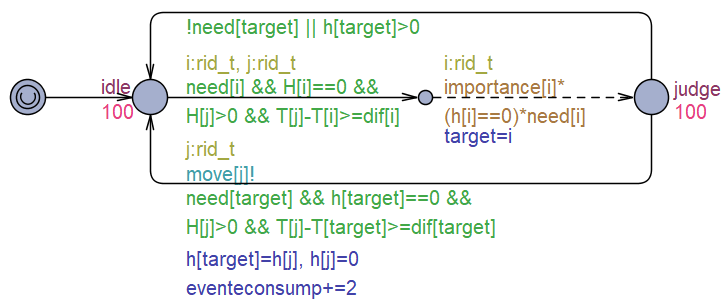
\includegraphics[width=1.05\textwidth]{scheduler-esha1.png} 
	\end{minipage}
	\label{scheduler1-esha}
	}
	\subfigure[strategy2]{
	\begin{minipage}[b]{0.4\textwidth}
	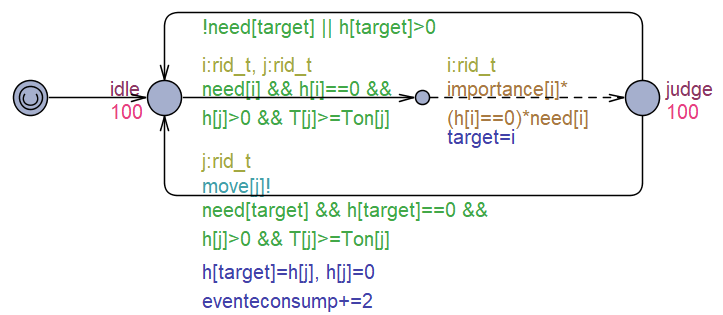
\includegraphics[width=1.05\textwidth]{scheduler-esha2.png} 
	\end{minipage}
	\label{scheduler2-esha}
	}
	\subfigure[strategy3]{
	\begin{minipage}[b]{0.4\textwidth}
	\includegraphics[width=1.05\textwidth]{scheduler-esha3.png} 
	\end{minipage}
	\label{scheduler3-esha}
	}
	\caption{三种策略的ESHA模型}
	\label{scheduler-esha}
	\end{figure}
	
	在现实生活中,为了鼓励人们错开用电高峰期,不同时段的电价是不相同的,对此,参考\citep{刘经浩2015一种基于实时电价的}我们构建了如图\ref{price}所示的实时电价ESHA模型。对于办公建筑,10点至14点是用电高峰期,此时的电价高于其他时间。
	
	\begin{figure}[!t]
	\centering
	\includegraphics[width=3.8in]{price.png}
	\caption{实时电价的ESHA模型}
	\label{price}
	\end{figure}
	
\subsection{模型验证与分析}
\textbf{1、模型仿真}

	由于在本案例中,共有4种不同的物理环境模型、3种不同的调度策略和3种不同的用户行为模式,因此共有$4\times3\times3$种组合情况。首先,我们采用固定配置$(weatherGauss,strategy1,work/out)$对模型进行仿真,来探究系统的能耗等性质。图\ref{T}为某次仿真48小时内六个房间室内环境温度变化情况。从图中可以看出在8(32)到14(38)时之间,各房间的温度均维持在16度以上,这说明调度器的智能控制起了作用,使得不会有房间的温度过低。在38到42时房间的温度有所下降,是由于用户出差离开了办公室,导致办公建筑开启夜间模式所致。图\ref{energy-discomfort}为10次仿真下48小时内能耗和用户不舒适度情况。受到外界环境的影响,在0到12时和24到36时,由于物理环境温度过低,需要加热器大量耗能来对办公建筑进行加热,因此在这两个阶段,能量消耗较快。而用户的不舒适度同样也是在上述两个夜间阶段增幅较大,其余时间较为稳定,说明调度器的调度有效,在白天办公场景中,为用户提供了一个较舒适的环境。
	
	\begin{figure}
	\centering
	\subfigure[48小时内各房间的温度]{
	\begin{minipage}[b]{0.4\textwidth}
	\includegraphics[width=1\textwidth]{T.png} 
	\end{minipage}
	\label{T}
	}
	\subfigure[48小时内系统能耗和用户不舒适度]{
	\begin{minipage}[b]{0.4\textwidth}
	\includegraphics[width=1\textwidth]{energy-discomfort.png} 
	\end{minipage}
	\label{energy-discomfort}
	}
	\caption{系统仿真结果}
	\label{simulation}
	\end{figure}

\textbf{2、模型验证与分析}

	在以下情形中,我们将物理环境固定为weatherGauss模式,以探究不同调度策略和用户模式对系统能耗、用户不舒适度和电费的影响。
	
	\textbf{不同策略}:	
	
	为了验证不同策略对系统变量的影响,我们固定用户行为模式为工作/出差模式。
	图\ref{3strategy}所示为调度器的三种不同策略下,用户不舒适度、系统能耗和电费的概率密度图。由图(a)可知,在48小时内关于用户不舒适度的平均值,$strategy2<strategy3<strategy1$,即策略$\uppercase\expandafter{\romannumeral2}$能为用户提供一个更为适宜的温度环境;由图(b)可知,在48小时内关于系统能耗的平均值,$strategy2<strategy3<strategy1$,即策略$\uppercase\expandafter{\romannumeral2}$更加节能;由图(c)可知,在48小时内关于电费的平均值,$strategy1<strategy2<strategy3$,即策略$\uppercase\expandafter{\romannumeral1}$能够使得电费总额最小,但是三种策略的差异并不明显;综合以上三点考虑可知,策略$\uppercase\expandafter{\romannumeral2}$在能够在使得系统能耗和电费较少的情况下,提供更好的用户舒适度,其性能最优。
	
	\begin{figure}
	\centering
	\subfigure[用户不舒适度]{
	\begin{minipage}[b]{0.4\textwidth}
	\includegraphics[width=1\textwidth]{s-dis.png} 
	\end{minipage}
	\label{dis-strategy}
	}
	\subfigure[系统能耗]{
	\begin{minipage}[b]{0.4\textwidth}
	\includegraphics[width=1\textwidth]{s-energy.png} 
	\end{minipage}
	\label{energy-strategy}
	}
	\subfigure[电费]{
	\begin{minipage}[b]{0.4\textwidth}
	\includegraphics[width=1\textwidth]{s-price.png} 
	\end{minipage}
	\label{price-strategy}
	}
	\caption{三种策略对用户不舒适度、系统能耗、电费的影响}
	\label{3strategy}
	\end{figure}
	
	\textbf{不同用户行为模式}:
	
	为了分析不同的用户行为模式对系统变量的影响,我们将调度器策略固定为strategy1,在此配置下验证了三种用户行为模式对用户不舒适度、系统能耗和电费的影响,实验结果如图\ref{3user}所示。由图(a)可知,会议模式的用户不舒适度均值最低,工作/出差模式下的用户不舒适度均值最高,这是由于会议室的权重最高,调度器会优先维持会议室的温度,而工作/出差模式下用户的随机行为给调度器的智能控制带来了障碍;由图(b)可知系统能耗与用户的工作时间密切相关。在会议模式下,用户的工作时间为8小时,日常工作模式下用户的工作时间为6小时。对于工作/出差模式,用户的工作时间为$4+4 \times 0.8=7.2$小时。图(b)所示与上述分析一致,会议模式下系统能耗最高,日常工作模式下系统能耗最低;由图(c)可知,关于电费总额,工作/出差模式<日常工作模式<会议模式,这是由于电费与能耗值密切相关,会议室的能耗速率最高,且下午召开会议时,实时电价最高。
	
	\begin{figure}
	\centering
	\subfigure[用户不舒适度]{
	\begin{minipage}[b]{0.4\textwidth}
	\includegraphics[width=1\textwidth]{u-dis.png} 
	\end{minipage}
	\label{dis-strategy}
	}
	\subfigure[系统能耗]{
	\begin{minipage}[b]{0.4\textwidth}
	\includegraphics[width=1\textwidth]{u-energy.png} 
	\end{minipage}
	\label{energy-strategy}
	}
	\subfigure[电费]{
	\begin{minipage}[b]{0.4\textwidth}
	\includegraphics[width=1\textwidth]{u-price.png} 
	\end{minipage}
	\label{price-strategy}
	}
	\caption{三种用户行为模式对用户不舒适度、系统能耗、电费的影响}
	\label{3user}
	\end{figure}
	

\section{本章小结}
	智能建筑中的一个典型实例是智能温控系统,本章基于一个温控系统的benchmark,设计了一个更符合实际情境的实验案例,并将本文提出的智能建筑的能耗建模与分析方法进行了应用:从系统的需求出发,利用领域本体辅助构建扩展的MARTE/UML模型,模型转换为ESHA,最终利用UPPAAL-SMC工具实现了系统能耗等性质的验证与分析,探究了不同的调度策略和用户随机行为对系统能耗的影响。

	
	
	

\chapter{总结与展望}
\label{ch6}



\input {C7-CHAP7.tex}

\clearpage

\addcontentsline{toc}{chapter}{参考文献}
\bibliographystyle{GBT7714-2005}
\bibliography{bib/tex}


\pagestyle{plain}
\clearpage
\phantomsection
\addcontentsline{toc}{chapter}{致谢}
{\kaishu
{\chapter*{\vspace{-3cm} 致\qquad 谢}}

\vspace{-0.5cm}

\begin{center} 
\end{center}
	
	在此论文完成之际,我首先要感谢我的导师杜德慧。她严肃的科学态度,严谨的治学精神以及精益求精的工作作风深深地感染和激励着我。从课题的选择到项目的最终完成,杜老师都始终给予我细心的指导和不懈的支持。两年来,她不仅在学业上给我以精心指导,同时还在思想、生活上给我以无微不至的关怀与照顾,在此谨向杜老师致以诚挚的谢意和崇高的敬意。

	感谢在研究生学习期间给我诸多教诲和帮助的软件学院的各位老师和同学、以及和我一起生活两年的室友,你们的执着、勤奋、以及对生活的态度,值得我学习。特别的,我要感谢辅导员张炜帆对我思想以及生活上的帮助,给我带来了莫大的帮助。

	最后感谢我的家人,你们不仅给我经济上的支持,同时还在我成长道路上无私地给予莫大支持与鼓励,让我独立地选择自己的人生道路。

\vspace{0.2cm} \hspace{11.5cm} 

\hspace{10.6cm}  二〇一七年十月 }

\pagestyle{plain}
\clearpage
\phantomsection
\addcontentsline{toc}{chapter}{发表论文和科研情况}
\section*{攻读硕士学位期间发表论文}

\vskip 5mm

{\heiti $\blacksquare$ 已公开发表论文}\vskip 5mm

\begin{enumerate}

  \item Yujie Yuan, Lihua Xu, Xusheng Xiao, Andy Podgurski, and Huibiao Zhu,RunDroid: Recovering Execution Call Graphs for Android Applications. In Proc. ESEC/FSE, 2017
  \eat{
  	\item xxxx  Proceedings of the IEEE Conference on Computer Vision and Pattern Recognition xxxxx 为模式识别和计算机视觉的三大国际顶级会议,中国计算机协会列为A类会议,根据猲猰猱猷年谷歌学术统计,h5-index排名所有学术刊物第35位,位列工程和计算机领域所有学术刊物第一位。 
  	注:第二作者,导师第一作者。xxxx是中国计算机协 会A类、图像处理领域的顶级期刊,SCI II区。
  }

\end{enumerate}





\printindex
\end{document}

